\chapter{Experimentos y resultados}
\label{ch:results}

En este capítulo presentaremos los experimentos principales realizados a partir
de lo desarrollado en el capítulo \ref{ch:method}. Entrenaremos 2 grupos de
modelos predictivos. Un grupo con una codificación ad-hoc, y otro grupo con una
codificación por word embeddings. Los vectores de características tendrán como
información una ventana del plan relajado y una acción. Se destacarán aquellos
modelos que presenten mejores resultados en validación cruzada y sobre ejemplos
del conjunto de test. Para aquellos modelos que tuvieron un mal desempeño,
mencionaremos algunas de las posibles causas.

Por otro lado se entrenarán los 3 algoritmos de clasificación vistos en el
capítulo \ref{ch:lit_ml}, \emph{XGBoost}, \emph{regresión logística}, y
\emph{perceptrón multicapa}. Los conjuntos de entrenamiento y de test son
divididos por esquemas de acción, entrenando un modelo por cada uno. Esto con el
fin de capturar la información significativa de un solo esquema por modelo. En
resumen, la estructura de nuestros experimentos para ambos grupos es la
siguiente:

\begin{itemize}
    \item Codificación ad-hoc o por word embeddings:
    \begin{itemize}
        \item Regresión logistica:
        \begin{itemize}
            \item \verb|take_image|
            \item \verb|turn_to|
            \item \verb|calibrate|
            \item \verb|switch_on|
            \item \verb|switch_off|
        \end{itemize}
        \item XGBoost:
        \begin{itemize}
            \item \verb|take_image|
            \item \verb|turn_to|
            \item \verb|calibrate|
            \item \verb|switch_on|
            \item \verb|switch_off|
        \end{itemize}
        \item Redes neuronales:
        \begin{itemize}
            \item \verb|take_image|
            \item \verb|turn_to|
            \item \verb|calibrate|
            \item \verb|switch_on|
            \item \verb|switch_off|
        \end{itemize}
    \end{itemize}
\end{itemize}

Por último, mencionaremos otros experimentos que se trabajaron durante la tesis,
que a pesar de no lograr el resultado que esperábamos, fueron muy importantes
para guiar futuros experimentos.

\section{Modelos predictivos por word embeddings}
\label{exp:ad-hoc}

\subsection{Configuración del experimento}

En primer lugar, se necesito asignar la configuración para la construcción de
las ventanas y planes relajados.  Observamos que por lo general los planes
relajados del conjunto de entrenamiento suelen tener entre $3$ a $10$ acciones.
Nuestro algoritmo debe ser capaz de generalizar para ejemplos de entrenamientos
no antes visto, por lo que el preprocesamiento que realicemos sobre estos datos
debe ser orientado a reducir las discrepancias entre un ejemplo nuevo y los que
fueron utilizados en la etapa de entrenamiento. Como el largo de los planes
relajados de los problemas de test es por encima de los cientos de acciones,
generamos ventanas que aproximen en en tamaño a los planes relajados de los
problemas de entrenamiento. Es por ello, que optamos por un paso y tamaño de
ventana de $3$.

Para el entrenamiento de los clasificadores, se realizó una búsqueda de
hiper-parámetros cuya métrica a optimizar es $H_{\beta}$ con $\beta = 1.5$. Dado
que en nuestro problema es más importante predecir correctamente todas las
acciones relevantes, optamos por priorizar la taza de verdaderos positivos sobre
la taza de verdaderos negativos. Es decir, buscamos que el clasificador sea
penalizado si no logra predecir todas las acciones relevantes para obtener un
plan, y si no logra filtrar una cantidad aceptable de acciones no relevantes.

Recordemos que para evaluar los modelos, generamos las predicciones a nivel de
ventana de plan relajado y acción. No obstante, buscamos predecir si una acción
es relevante dada la información del plan relajado completo, por lo que es
necesario agrupar las predicciones que cada ventana realizó sobre esa acción.
Por ejemplo, supongamos que tenemos $M$ ventanas de un plan relajado $\vec{a}$
de una tarea $\Pi$ y se busca determinar la probabilidad de una acción $a'$ dado
$\vec{a}$. El modelo de aprendizaje automático propuesto realiza $M$
predicciones para $a'$ dado las $M$ ventanas de $\vec{a}$ donde cada estimación
es una probabilidad. En lugar de evaluar el modelo con las $M$ predicciones, las
agrupamos para obtener solo una. Para este experimento, seleccionamos el máximo
de las $M$ probabilidades. Notar que bajo esta decisión, una probabilidad baja
significa que para todas las ventanas del plan relajado, el planificador le
asignó una baja probabilidad a $a'$, mientras que una probabilidad alta requiere
que por lo menos una ventana del plan relajado haya provisto la información
necesaria para considerar relevante a $a'$.

Por último, los algoritmos presentados en el capítulo \ref{ch:lit_ml}
implementan una solución genérica de los métodos de aprendizaje. Por lo que se
requiere especificar como van a estar configurados antes de empezar el proceso
de entrenamiento. La siguiente lista de parámetros muestra aquellos que fueron
utilizados para cada algoritmo en este experimento:

\begin{conditions}
\emph{Nombre\ del\ modelo} & \verb|Regresión logística| \\
\emph{penalty} & \verb|[elasticnet]| \\
\emph{C} & \verb|[1, 0.1, 0.01]| \\
\emph{class\_weight} & \verb|[balanced]|  \\
\emph{solver} & \verb|[saga]|  \\
\emph{max\_iter} & \verb|[1000 10000]| \\
\emph{random\_state} & \verb|[0]| \\
\emph{l1\_ratio} & \verb|[0, 1]|
\end{conditions}

\begin{conditions}
\emph{Nombre\ del\ modelo} & \verb|XGBoost| \\
\emph{objective} & \verb|[binary:logistic]| \\
\emph{n\_estimators} & \verb|[500, 1000]| \\
\emph{gamma} & \verb|[0.001, 1]| \\
\emph{max\_depth} & \verb|[10, 20]| \\
\emph{alpha} & \verb|[0.001, 1]| \\
\emph{lambda} & \verb|[0.001, 1]| \\
\emph{booster} & \verb|[gbtree]| \\
\emph{colsample\_bytree} & \verb|[1]| \\
\emph{subsample} & \verb|[0.5]| \\
\emph{eval\_metric} & \verb|[logloss]| \\
\emph{use\_label\_encoder} & \verb|[false]| \\
\emph{random\_state} & \verb|[0]|
\end{conditions}

\begin{conditions}
\emph{Nombre\ del\ modelo} & \verb|PytorchNN| \\
\emph{h\_size} & \verb|[32, 64]| \\
\emph{n\_layers} & \verb|[2, 4, 8, 16]| \\
\emph{bn\_bool} & \verb|[False]| \\
\emph{p} & \verb|[0, 0.1]| \\
\emph{epochs} & \verb|[20]| \\
\emph{batch\_size} & \verb|[32]| \\
\emph{balanced} & \verb|[True]| \\
\emph{lr} & \verb|[0.001]| \\
\end{conditions}

Estos parámetros corresponden con la interfaz provista por las librerías de
\emph{Scikit-learn} y \emph{Pytorch} que implementan los algoritmos de
aprendizaje. Cada parámetro muestra una lista de uno o más valores donde cada
elemento representa una posible asignación de ese parámetro. La cantidad de
configuraciones posibles de un modelo es igual al producto cartesiano de cada
una de las listas de los parámetros de un modelo. Por ejemplo para el caso de la
regresión logística, los parámetros \emph{C}, \emph{max\_iter}, y
\emph{l1\_ratio} tienen 3, 2, y 2 asignaciones respectivamente, el resto de
parámetros solo tiene una. Por lo tanto, hay un total de $3 \times 2 \times 2 =
12$ configuraciones del modelo.

Los parámetros que seleccionamos siempre buscaban plantear variantes en la
función de costo a optimizar, el tipo de optimizador, y métodos para evitar el
sobreajuste. En particular, seguimos como guía valores comunes que la comunidad
de aprendizaje automático suele utilizar para estos modelos,  la experiencia
transmitida por el ´boca a boca´, y conocimientos tanto del área de planning
como del funcionamiento interno de los modelos utilizados. 

En el caso de la regresión logística, los parámetros \emph{penalty},
\emph{l1\_ratio}, y \emph{C} permiten realizar variaciones en la regularización
de la función de costo, evitando que la norma del vector de pesos del modelo
crezca demasiado por sobreajuste. \emph{solver} indica el método de optimización
de la función de costo. \emph{max\_iter} es el número de iteraciones que
requiere el algoritmo para converger. Por último, \emph{class\_weight} permite
configurar el modelo de tal manera que balancee la cantidad de ejemplares
positivos y negativos del material de entrenamiento. Este último es importante
para nosotros ya que nuestro conjunto de entrenamiento está desbalanceado,
teniendo una mayor cantidad de good operators que de bad operators por problema.

XGBoost requiere que se le especifiquen la cantidad de árboles a ensamblar con
\emph{n\_estimators}, la fuerza del parámetro de regularización \emph{gamma}, y
la profundidad máxima de los árboles \emph{max\_depth}. \emph{objetive} indica
la función objetivo a optimizar, en este caso la misma función de costo que una
regresión logística. \emph{booster} permite seleccionar variantes del método
iterativo de boosting explicado en el capítulo \ref{alg:xgboost}. Por último
\emph{colsample\_bytree} y \emph{subsample} permiten tomar una muestra con
reposición de las filas o columnas en la confección de un árbol en el ensemble
con el proposito de reducir el sobreajuste.

La red neuronal necesita del número de neuronas para todas las capas
\emph{h\_size}, la cantidad de capas ocultas \emph{n\_layers}, si los vectores
de entrada son normalizados \emph{bn\_bool}, y la probabilidad  \emph{p} de
apagar momentáneamente neuronas de la red de manera aleatoria.

Por cada posible asignación obtenemos aquella que mejor se comporte con el
conjunto de test. Recordemos que nuestro objetivo es encontrar modelos que se
puedan utilizar para algún esquema de acción. De un total de 5 esquemas de acción
en el dominio \emph{Satellite}, el mejor caso sería encontrar 5 modelos que den
buenos resultados en esos esquemas.

\subsection{Resultados: take\_image}

Empecemos por el esquema de acción \verb|take_image| con el cual obtuvimos
mejores resultados. De los 3 modelos regresión logística (LGR), xgboost (XGB), y
redes neuronales (NN), el que mejor comportamiento que obtuvimos fue con la
regresión logística. 

\begin{figure}[t!]
    \centering
    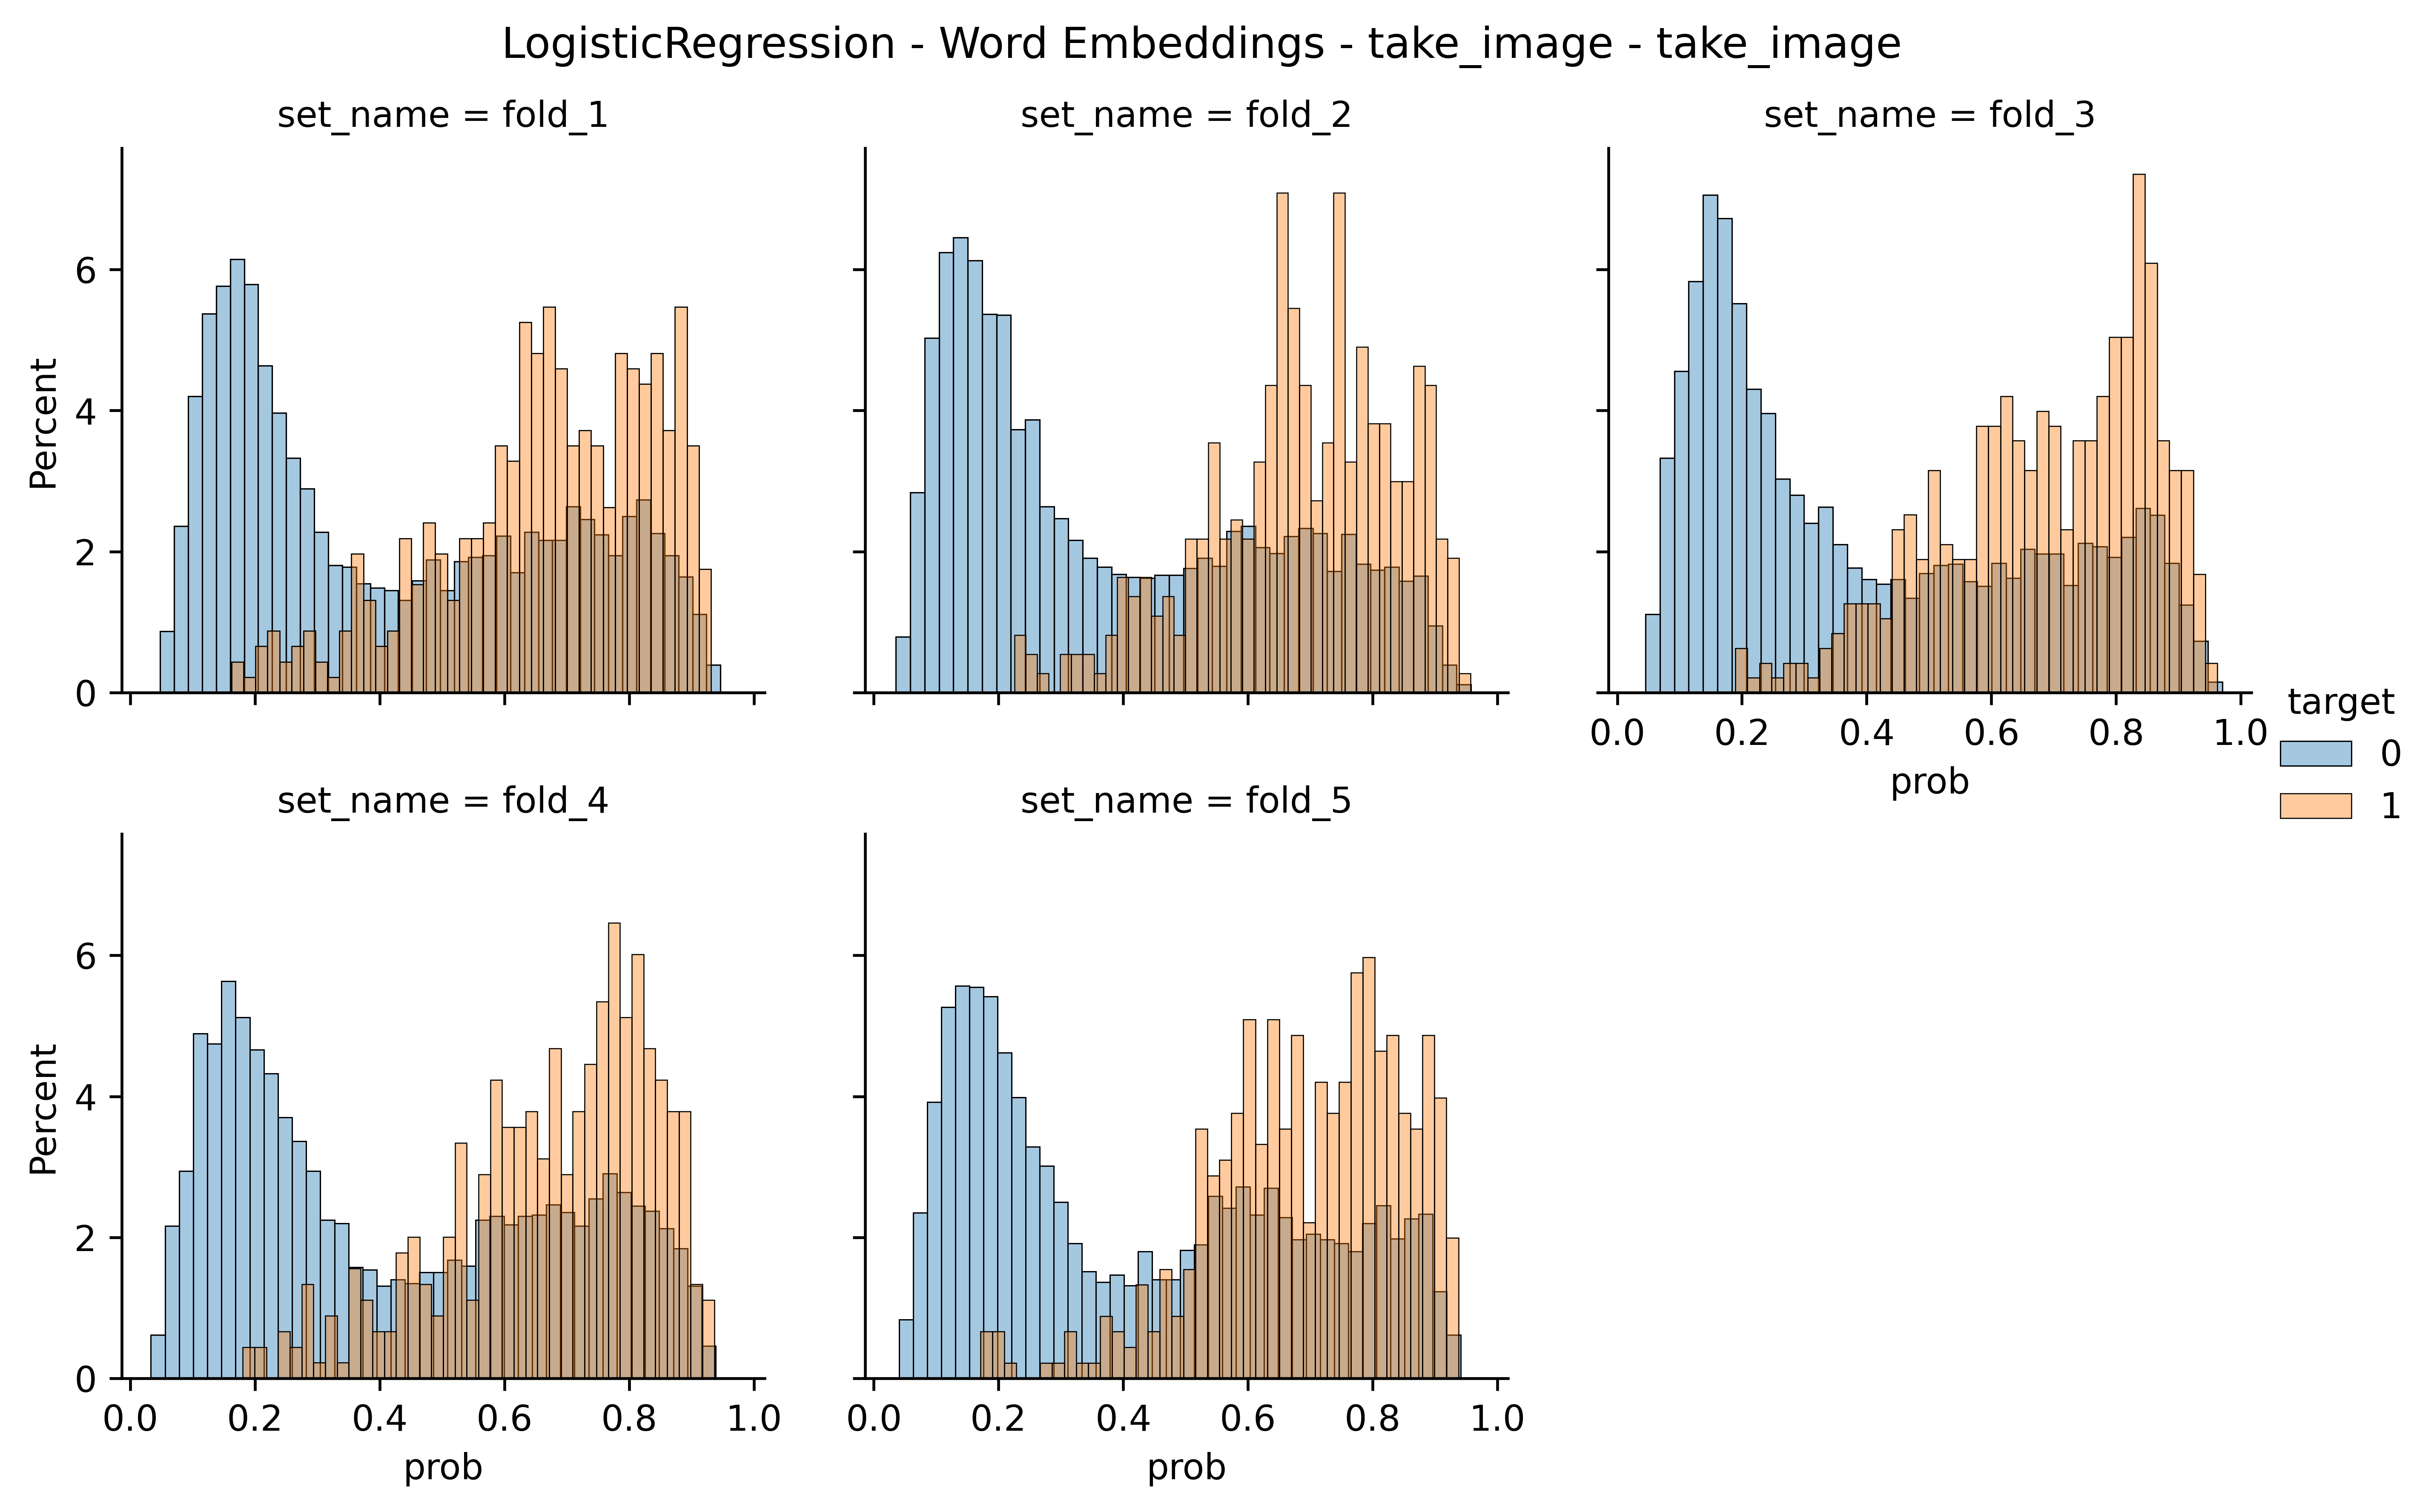
\includegraphics[width=\linewidth]{figures/results/word_embeddings/lgr/take_image/lgr_wb_take_image.png}
    \caption{Distribución de predicciones en validación cruzada para el modelo de LGR con word embeddings.}
    \label{fig:takeimage-bestmodel-distplot}
\end{figure}

\subsubsection{Performance en validación cruzada}

La figura \ref{fig:takeimage-bestmodel-distplot} muestra la distribución de las
predicciones en validación cruzada para la mejor configuración de parámetros de
LGR.


\begin{figure}[b!]
    \minipage{0.50\textwidth}
    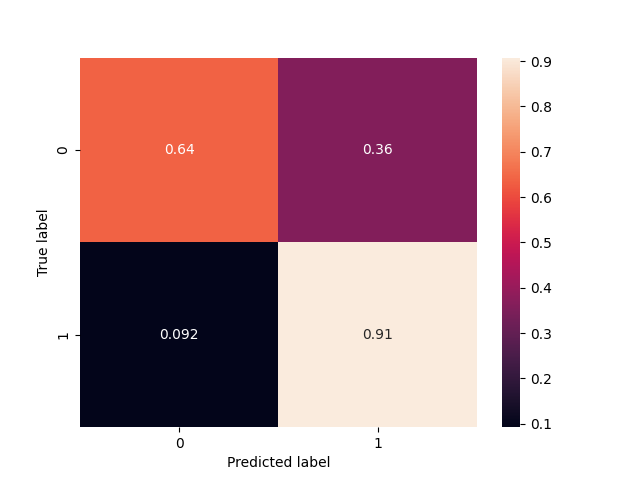
\includegraphics[width=\linewidth]{figures/results/word_embeddings/lgr/take_image/lgr_set_1_confusion_matrix_percent.png}
    \endminipage
    \minipage{0.50\textwidth}
    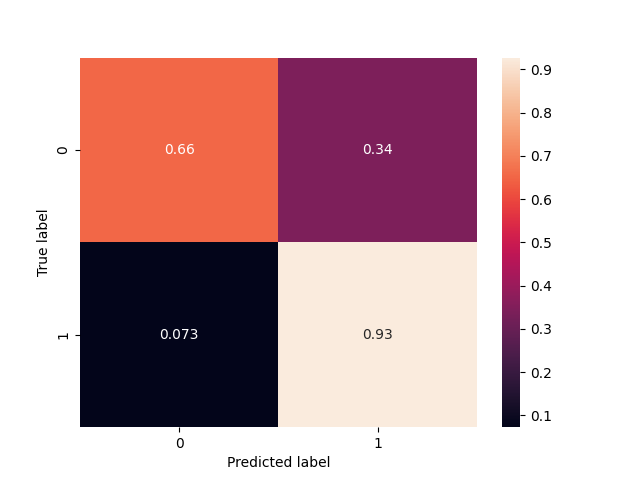
\includegraphics[width=\linewidth]{figures/results/word_embeddings/lgr/take_image/lgr_set_2_confusion_matrix_percent.png}
    \endminipage
        
    \minipage{0.50\textwidth}%
    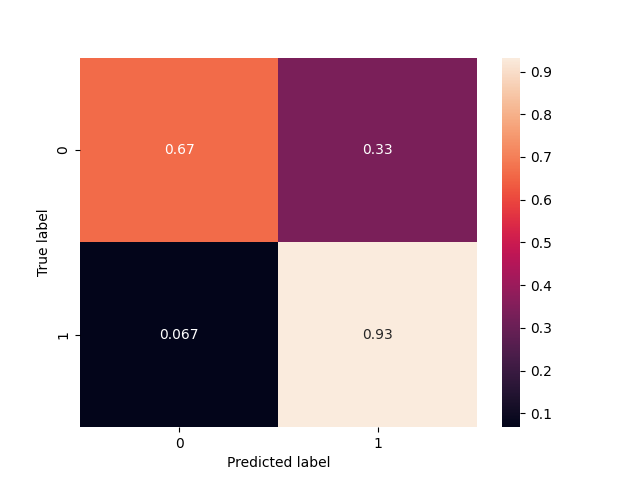
\includegraphics[width=\linewidth]{figures/results/word_embeddings/lgr/take_image/lgr_set_3_confusion_matrix_percent.png}
    \endminipage
    \minipage{0.50\textwidth}
    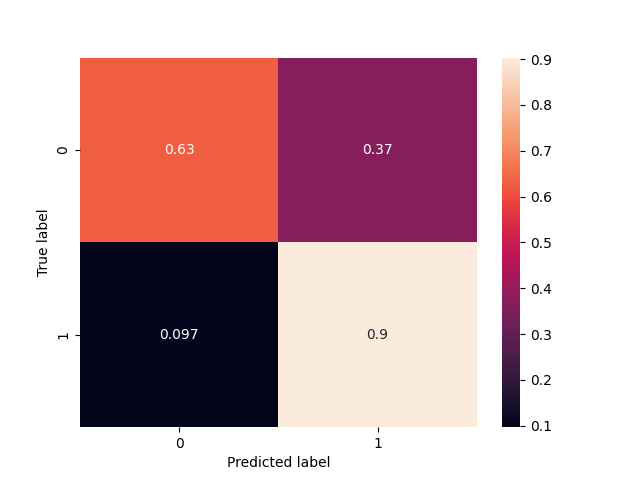
\includegraphics[width=\linewidth]{figures/results/word_embeddings/lgr/take_image/lgr_set_4_confusion_matrix_percent.png}
    \endminipage

    \minipage{0.50\textwidth}
      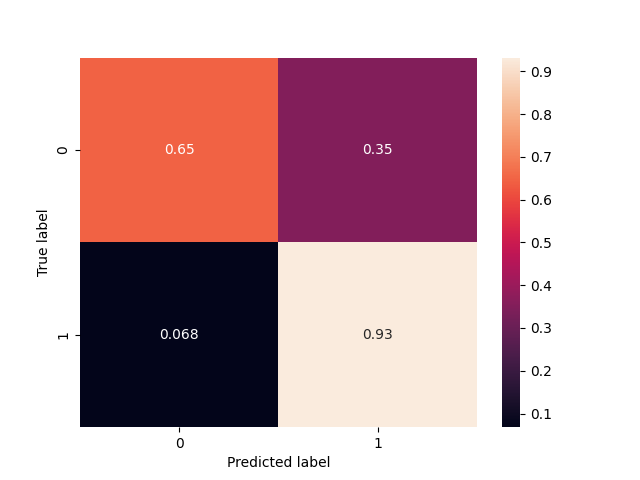
\includegraphics[width=\linewidth]{figures/results/word_embeddings/lgr/take_image/lgr_set_5_confusion_matrix_percent.png}
    \endminipage
    \caption{Matrices de confusión en validación cruzada para el modelo de LGR con word embeddings.}
    \label{fig:takeimage-bestmodel-cm}
\end{figure}

Para cada particiòn, se muestran dos histogramas independientes, el de la clase
positiva, y el de la clase negativa. Cada punto en el gráfico representa la
probabilidad de una acción dado su plan relajado (completo). En ambos
histogramas se genera una cantidad $N$ de bins equidistantes en el rango $[0;1]$.
Luego, para cada bin $b$, se muestra la cantidad de acciones que recibieron una
probabilidad contenida en $b$ divido el tamaño de la clase a la que pertenecen.

Para los histogramas de la clase positiva, observamos que las acciones relevantes
(good operators) se agrupan en los bins con probabilidades entre $r=[0,6; 1]$.
Cada bin contiene entre el 2\% al 7\% de las acciones. Si sumamos los
porcentajes de cada uno de los bins en $r$, tendremos que más de la mitad de las
acciones se encuentran en $r$.

Por otro lado, los histogramas de la clase negativa, muestran que más de la mitad
de las acciones no relevantes (bad operators) se agrupan en los bins con
probabilidades entre $[0;0.4]$.

Desde el punto de vista de grounding heurístico este es el comportamiento que
buscamos. El algoritmo almacenará en una cola de prioridades acciones tanto
relevantes como no relevantes con una probabilidad asociada, dándole prioridad a
las que tienen una mayor probabilidad. Si el modelo asigna a las acciones
relevantes una alta probabilidad entonces el proceso de grounding heurístico les
dará prioridad para su instanciación.

Notar que el objetivo de utilizar validación cruzada es variar el conjunto de
entrenamiento con el fin de determinar si el modelo de LGR es robusto ante
cambios, lo cual podemos decir que indudablemente fue este el caso en las 5
particiones.

Si observamos la matriz de confusión del modelo por cada partición dada por la
figura \ref{fig:takeimage-bestmodel-cm}, podemos ver que en cada uno, más del
90\% de las acciones positivas se predicen como positivas, y más del 63\% de las
negativas se predicen como negativas. La función de decisión se obtiene a partir
de optimizar $H_{1.5}$. Es decir, se computa $H_{1.5}$ para distintas
funciones de decisión con umbral en el intervalo [0, 1] y utilizamos aquel que
maximice $H_{1.5}$. 

\subsubsection{Performance en test}

Los resultados anteriores fueron sobre 5 particiones del conjunto de
entrenamiento donde una parte efectivamente se utilizaba para entrenar el modelo
y otra para su evaluación. Sin embargo, lo que buscamos es que esto mismo se
logre generalizar a problemas no instanciables. Por lo tanto, la evaluación
final la realizamos sobre el conjunto de test.

\begin{figure}[t!]
    \centering
    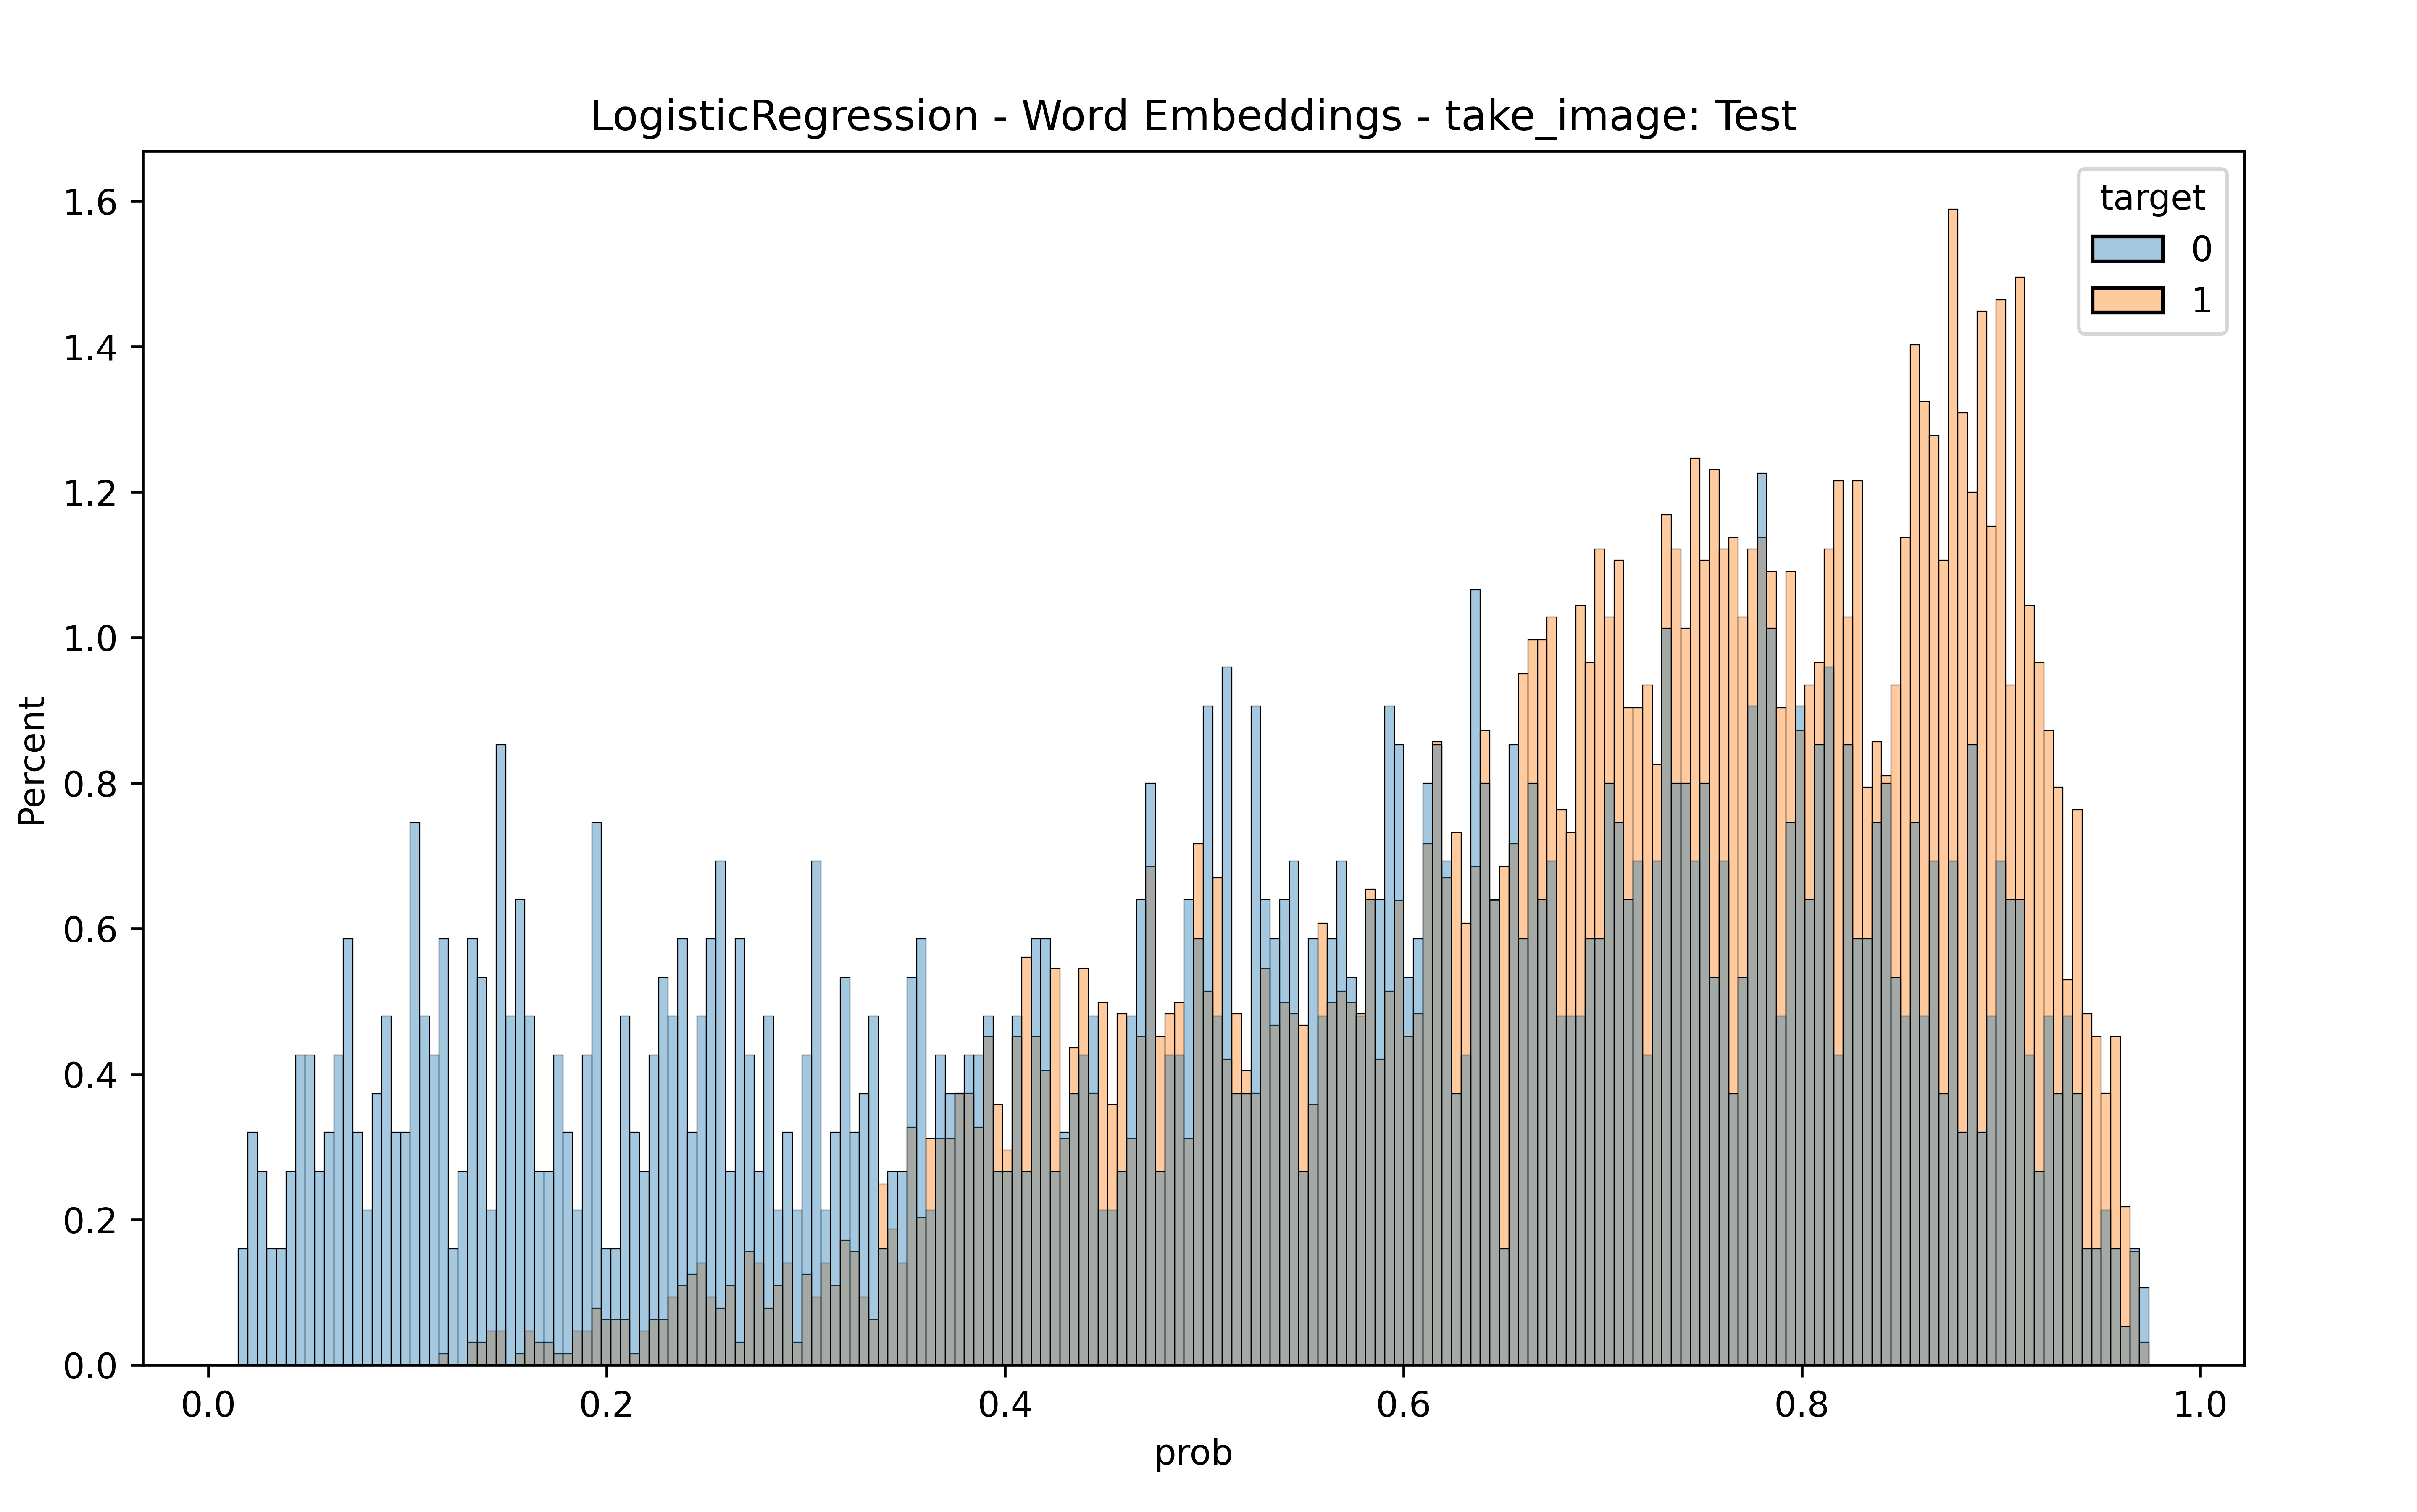
\includegraphics[width=0.7\linewidth]{figures/results/word_embeddings/lgr/take_image/lgr_wb_take_image_test.png}
    \caption{Distribución de predicciones sobre el conjunto de test del modelo de LGR con word embeddings.}
    \label{fig:takeimage-bestmodel-distplot-test}
\end{figure}

\begin{figure}[t!]
    \begin{subfigure}[b]{\textwidth}
        \centering
        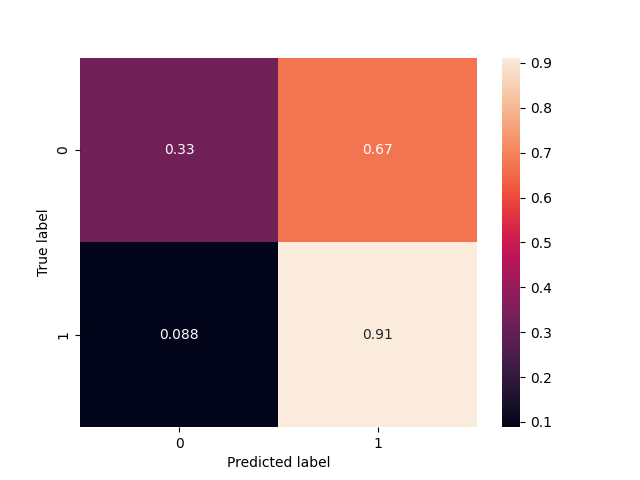
\includegraphics[width=0.7\linewidth]{figures/results/word_embeddings/lgr/take_image/lgr_set_6_confusion_matrix_percent.png}
        \caption{Matriz normalizada por clase}
        \label{fig:takeimage-bestmodel-cm-test}
    \end{subfigure}
    \begin{subfigure}[b]{\textwidth}
        \centering
        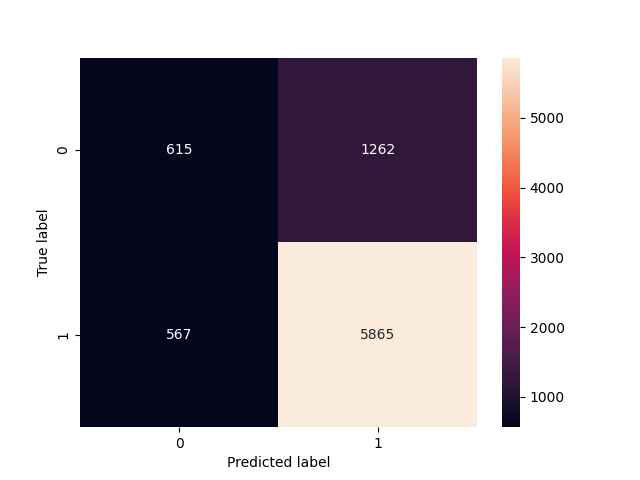
\includegraphics[width=0.7\linewidth]{figures/results/word_embeddings/lgr/take_image/lgr_set_6_confusion_matrix_raw.png}
        \caption{Matriz sin normalización}
        \label{fig:takeimage-bestmodel-cm-raw-test}
    \end{subfigure}
    \caption{Matrices de confusión sobre el conjunto de test del modelo de LGR con word embeddings.}
\end{figure}

La figura \ref{fig:takeimage-bestmodel-distplot-test} muestra nuevamente
un histograma de la probabilidad de una acción dado su plan relajado. Para el caso de
las acciones relevantes, se sigue manteniendo el comportamiento que vimos en
validación cruzada lo cual es un buen indicio ya que estarán en las primeras
posiciones en la cola de prioridades en grounding heurístico. Sin embargo, si
observamos el histograma de acciones no relevantes, se tiene que ahora a una
gran parte de ellas se le asigna una alta probabilidad. Estas acciones también
serían ubicadas al comienzo de la cola de prioridades y por lo tanto
instanciadas. Si observamos la matriz de confusión en la figura
\ref{fig:takeimage-bestmodel-cm-test}, la proporción de acciones relevantes se
mantiene en un 91\%, mientras que esta vez un 67\% de las no relevantes se
filtran como positivas, cabe recalcar que esta vez, el umbral de decisión en
test es el promedio de los umbrales obtenidos en validación cruzada. El objetivo
era aprender un umbral que sea lo más óptimo para predecir nuevos ejemplos,
utilizando únicamente información de los datos de entrenamiento. Podríamos haber
utilizado un umbral de decisión a partir de las etiquetas de test, no obstante
tal predicción representaría la performance máxima o ideal que podríamos obtener
en test, y no la que realmente estamos obteniendo con información del conjunto
de entrenamiento.

Si observamos la matriz de confusión de la figura
\ref{fig:takeimage-bestmodel-cm-raw-test} del modelo LGR, pero esta vez sin
normalizar por porcentajes. Se puede ver que LGR tiende a predecir ligeramente
sobre la clase positiva, pero además es la mayoritaria en test para este
esquema. Esto sucede debido a como se generan los bad operators en los problemas
de test. Recordemos que estos no pudieron obtenerse a través de Fast Downward,
por lo se generó una muestra aleatoria usando grounding cartesiano pero
respetando los tipos de las interfaces. Como solo se pudieron generar una
cantidad de 5000 bad operators por problema, y los planes en los problemas de
test son de mayor tamaño que los de entrenamiento, surgió este desbalance hacia
la clase positiva. No obstante, en una situación real, la cantidad de bad
operators sería nuevamente superior a la de good operators. Otro aspecto
importante sobre la generación de los bad operators es que podrían no ser
alcanzables relajadamente, y por lo tanto tener una distribución distinta a la
que tenemos en el conjunto de entrenamiento siendo una de las posibles causas
del desempeño de LGR para la clase negativa. Es decir, LGR fue entrenado para
predecir, sobre acciones alcanzables relajadamente, pero lo estamos evaluando
sobre bad operators que no lo son.

Por último, en el cuadro \ref{results:lgr-wb-calibrate} se puede ver que
precision y recall sobre la clase positiva es de 0.823, y 0.912,
respectivamente. Si calculamos la métrica $F_{1.5}$ priorizando recall,
obtendriamos una performance de 0.8826 para LGR. Sin embargo, no es un buen
indicio de la correctitud del modelo en la clase negativa. En contraparte, si en
lugar de considerar $F_{1.5}$ utilizamos $H_{1.5}$ la performance es de 0.589
debido a que esta métrica penaliza si se tiene un baja en la taza de verdaderos
negativos.


\begin{table}[t!]
\centering
\scalebox{1}{
 \begin{tabular}{|c || c | c | c | c | c | c |} 
 \hline
  Clase & Precisión & Recall & $H_{1.5}$ & $F_{1.5}$ & Umbral de decisión \\
 \hline
 Relevante & 0.823 & 0.912 & 0.589 & 0.8826 & 0.416 \\
 No relevante & 0.52 & 0.33 & 0.4081 & 0.3717 & 0.416 \\
 \hline
 \end{tabular}}
 \caption{Métricas sobre el conjunto de test del modelo de LGR con word embeddings.}
 \label{results:lgr-wb-calibrate}
\end{table}


% Por otro lado, el modelo de redes neuronales se comportó mucho mejor en
% validaciòn cruzada, como lo muestra la figura
% \ref{fig:nn-distplot-takeimage-wb}. Sin embargo el conjunto de test
% 
% \begin{figure}[b!]
%     \centering
%     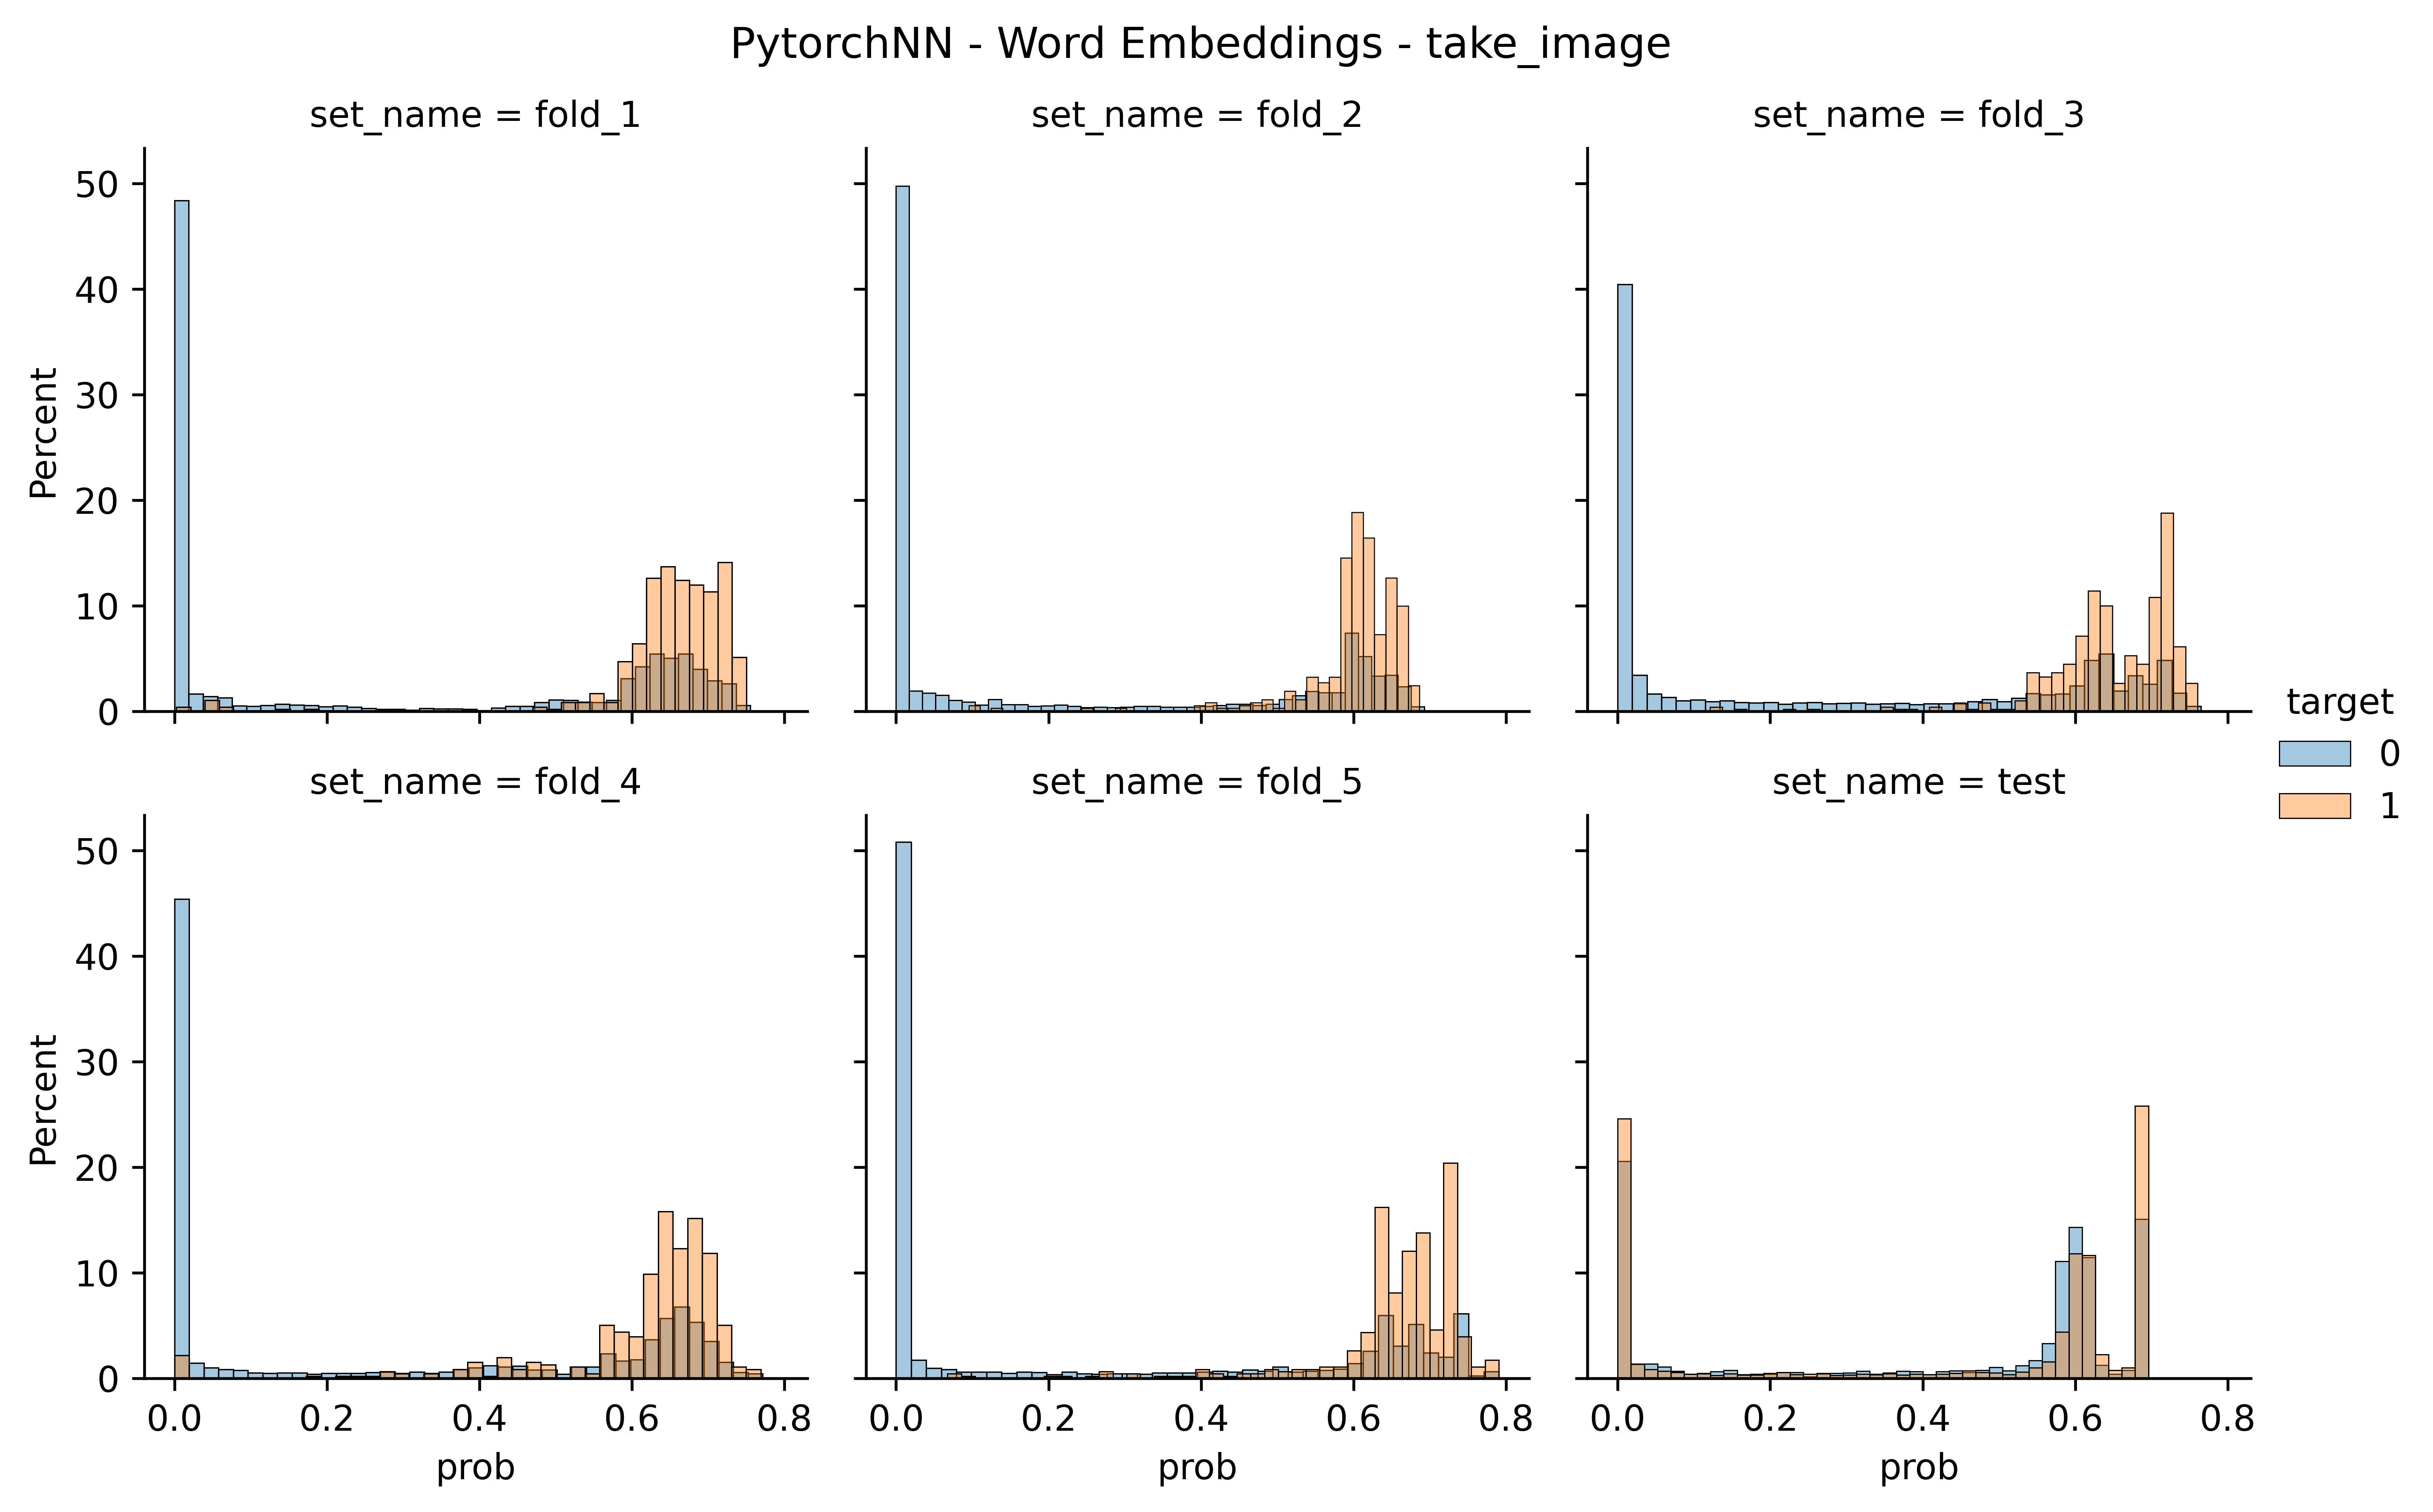
\includegraphics[width=\linewidth]{figures/results/word_embeddings/nn/take_image/take_image__distplot.png}
%     \caption{Distribución de predicciones en validación cruzada y el conjunto de test en take\_image para el modelo de redes neuronales.}
%     \label{fig:nn-distplot-takeimage-wb}
% \end{figure}
% \begin{figure}
%     \centering
%     \begin{subfigure}[b]{0.83\textwidth}
%     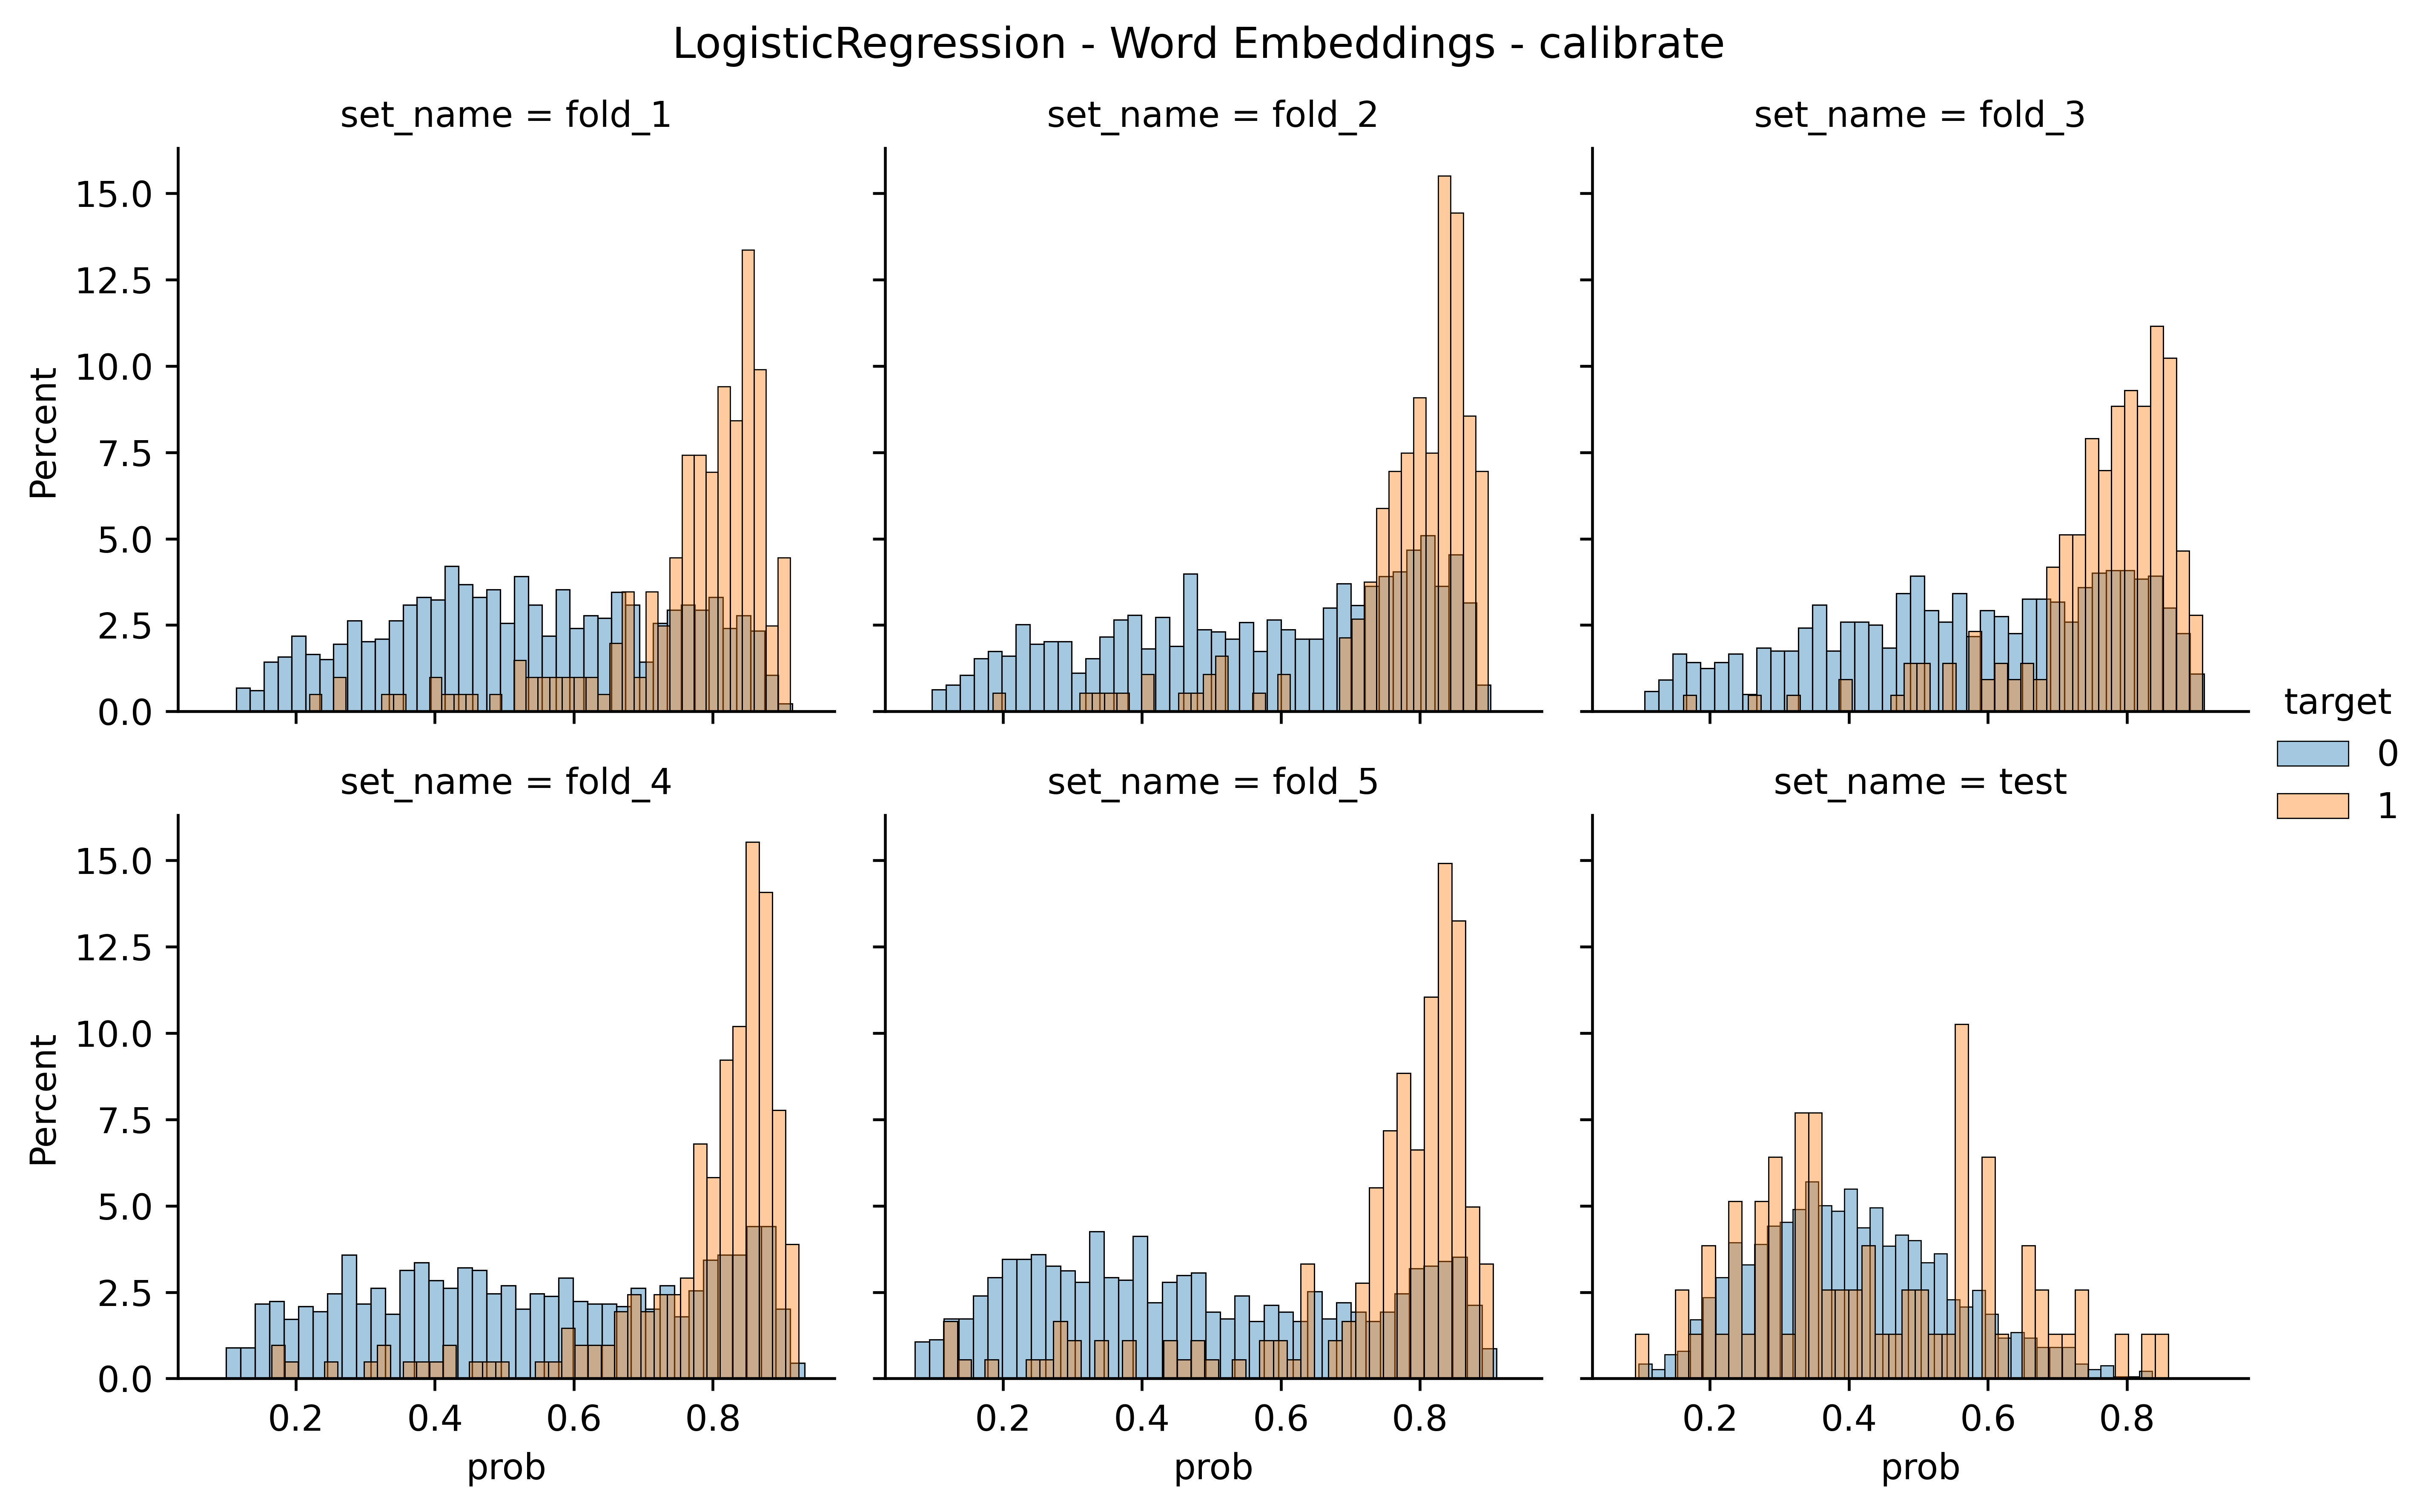
\includegraphics[width=\linewidth]{figures/results/word_embeddings/lgr/calibrate/calibrate__distplot.png}
%     \end{subfigure}
%     \hfill
%     \centering
%     \begin{subfigure}[b]{0.83\textwidth}
%         \centering
%         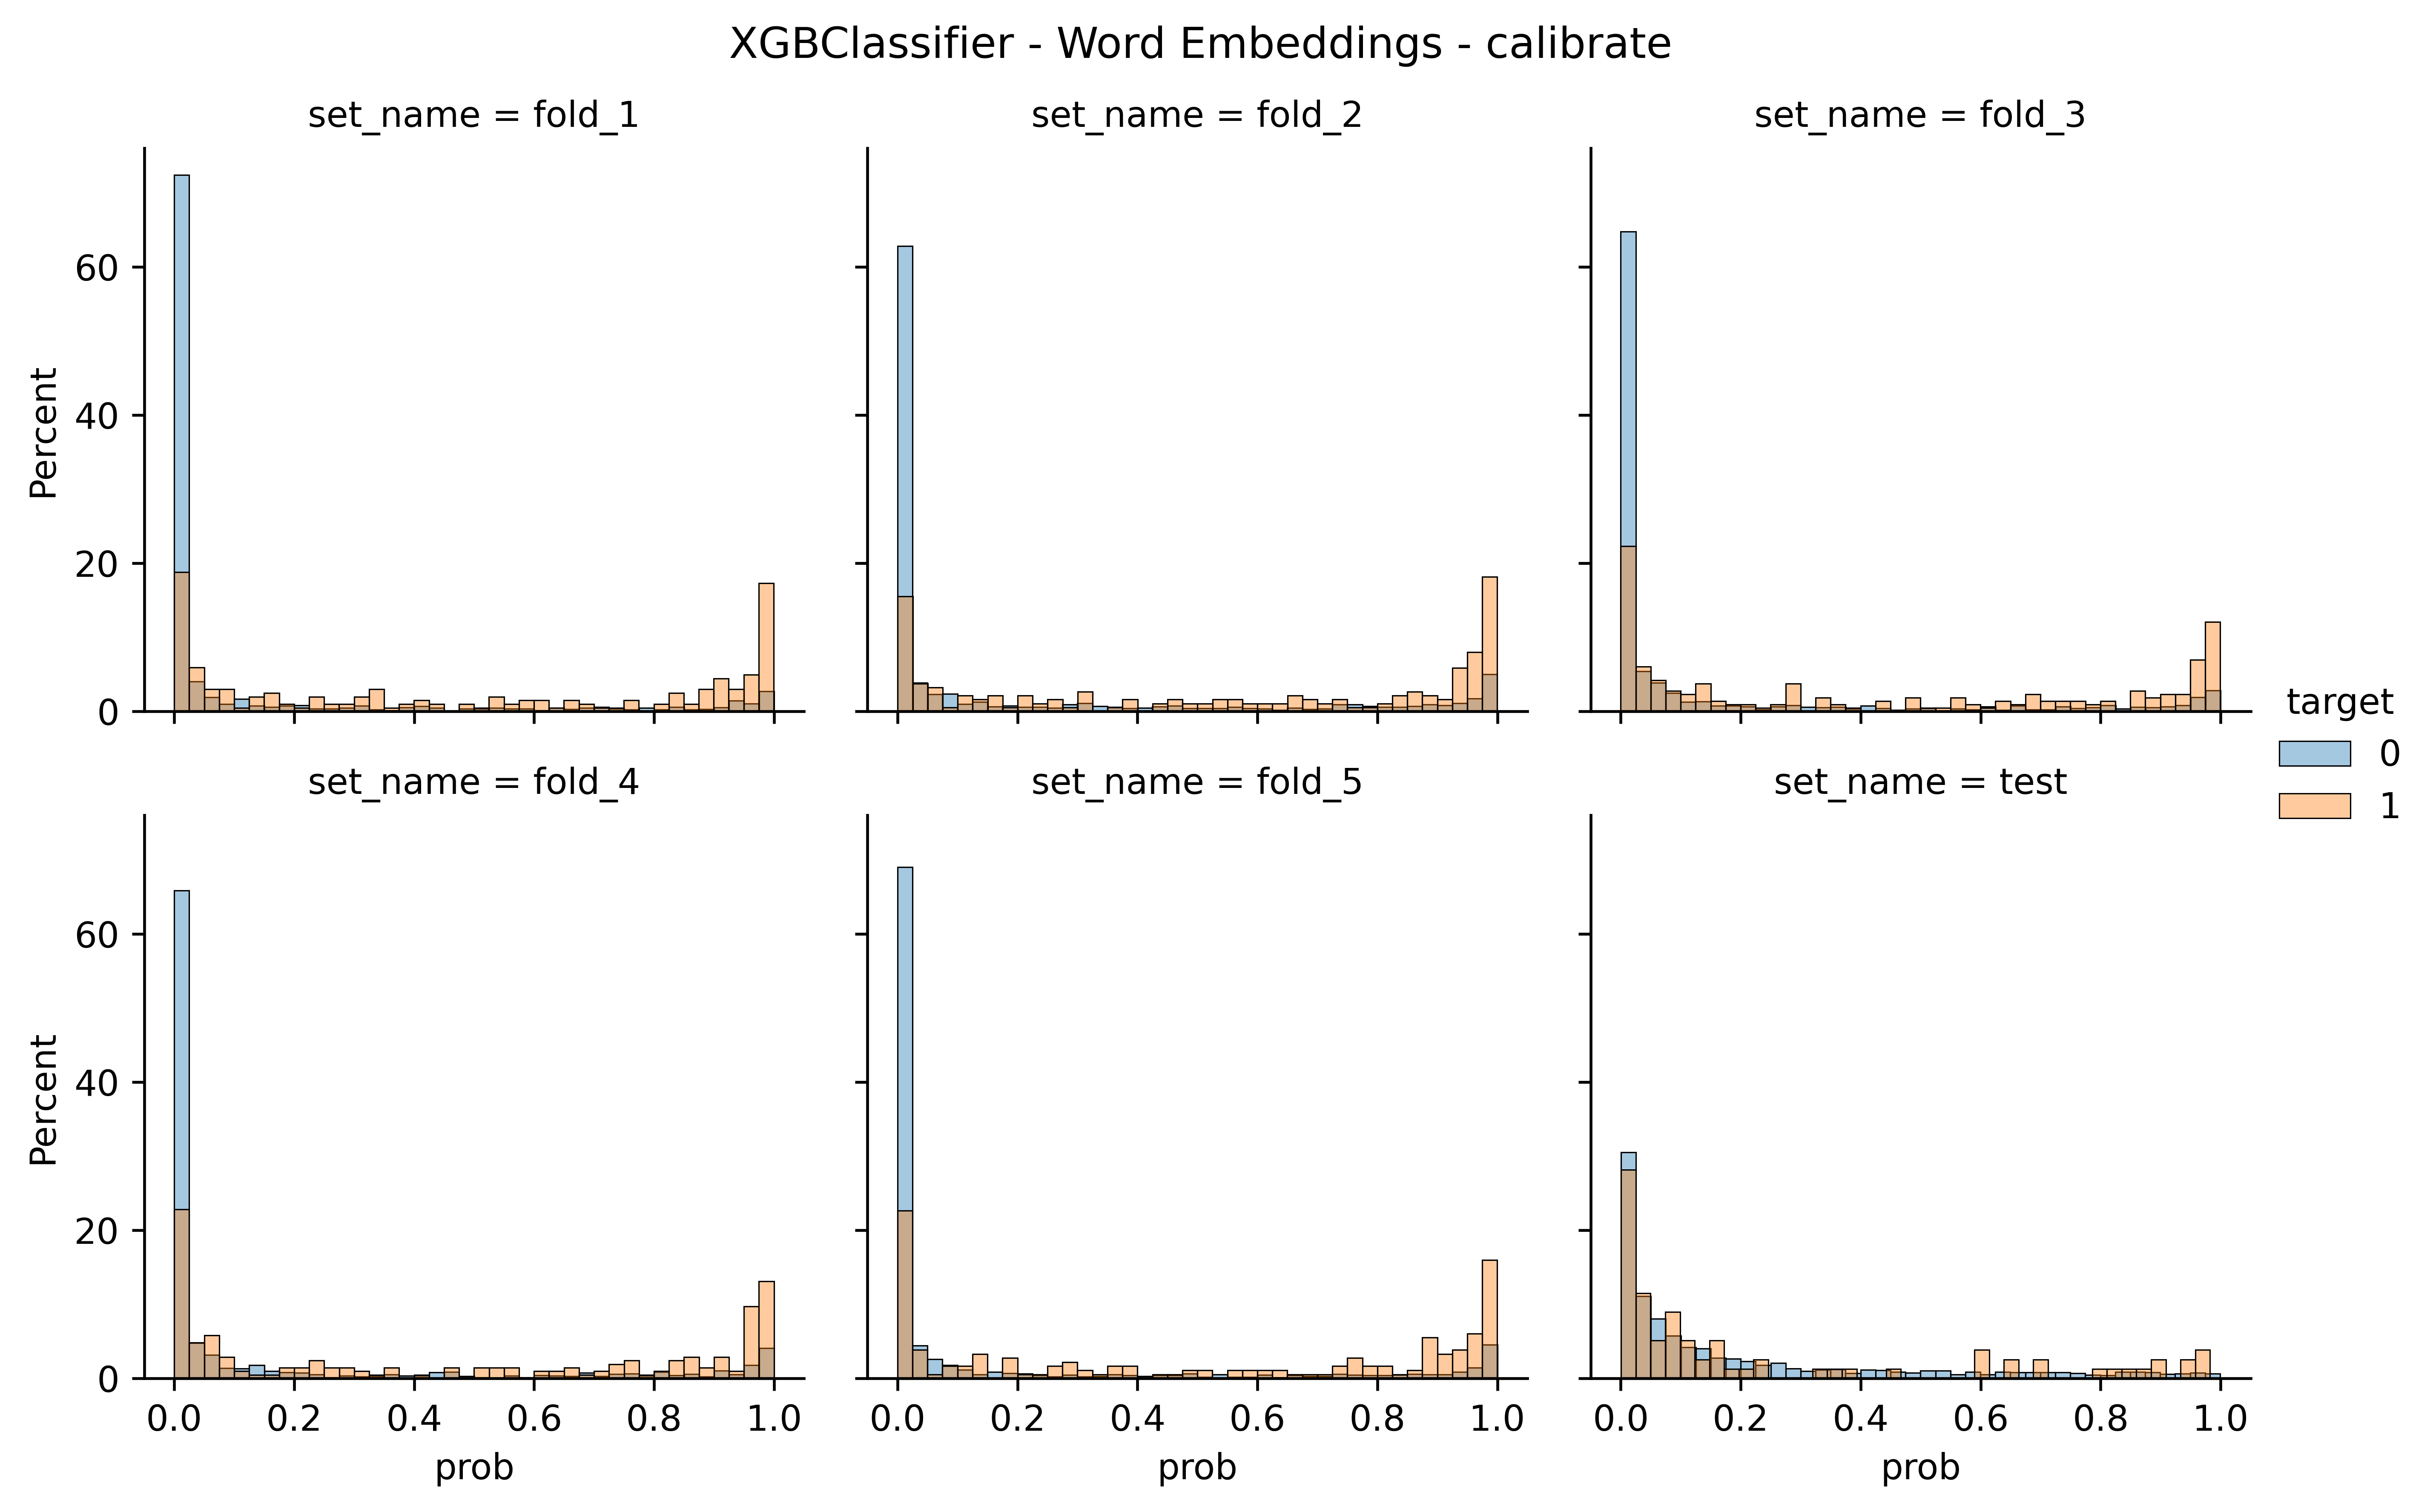
\includegraphics[width=\linewidth]{figures/results/word_embeddings/xgboost/calibrate/calibrate__distplot.png}
%     \end{subfigure}
%     \hfill
%     \centering
%     \begin{subfigure}[b]{0.83\textwidth}
%         \centering
%         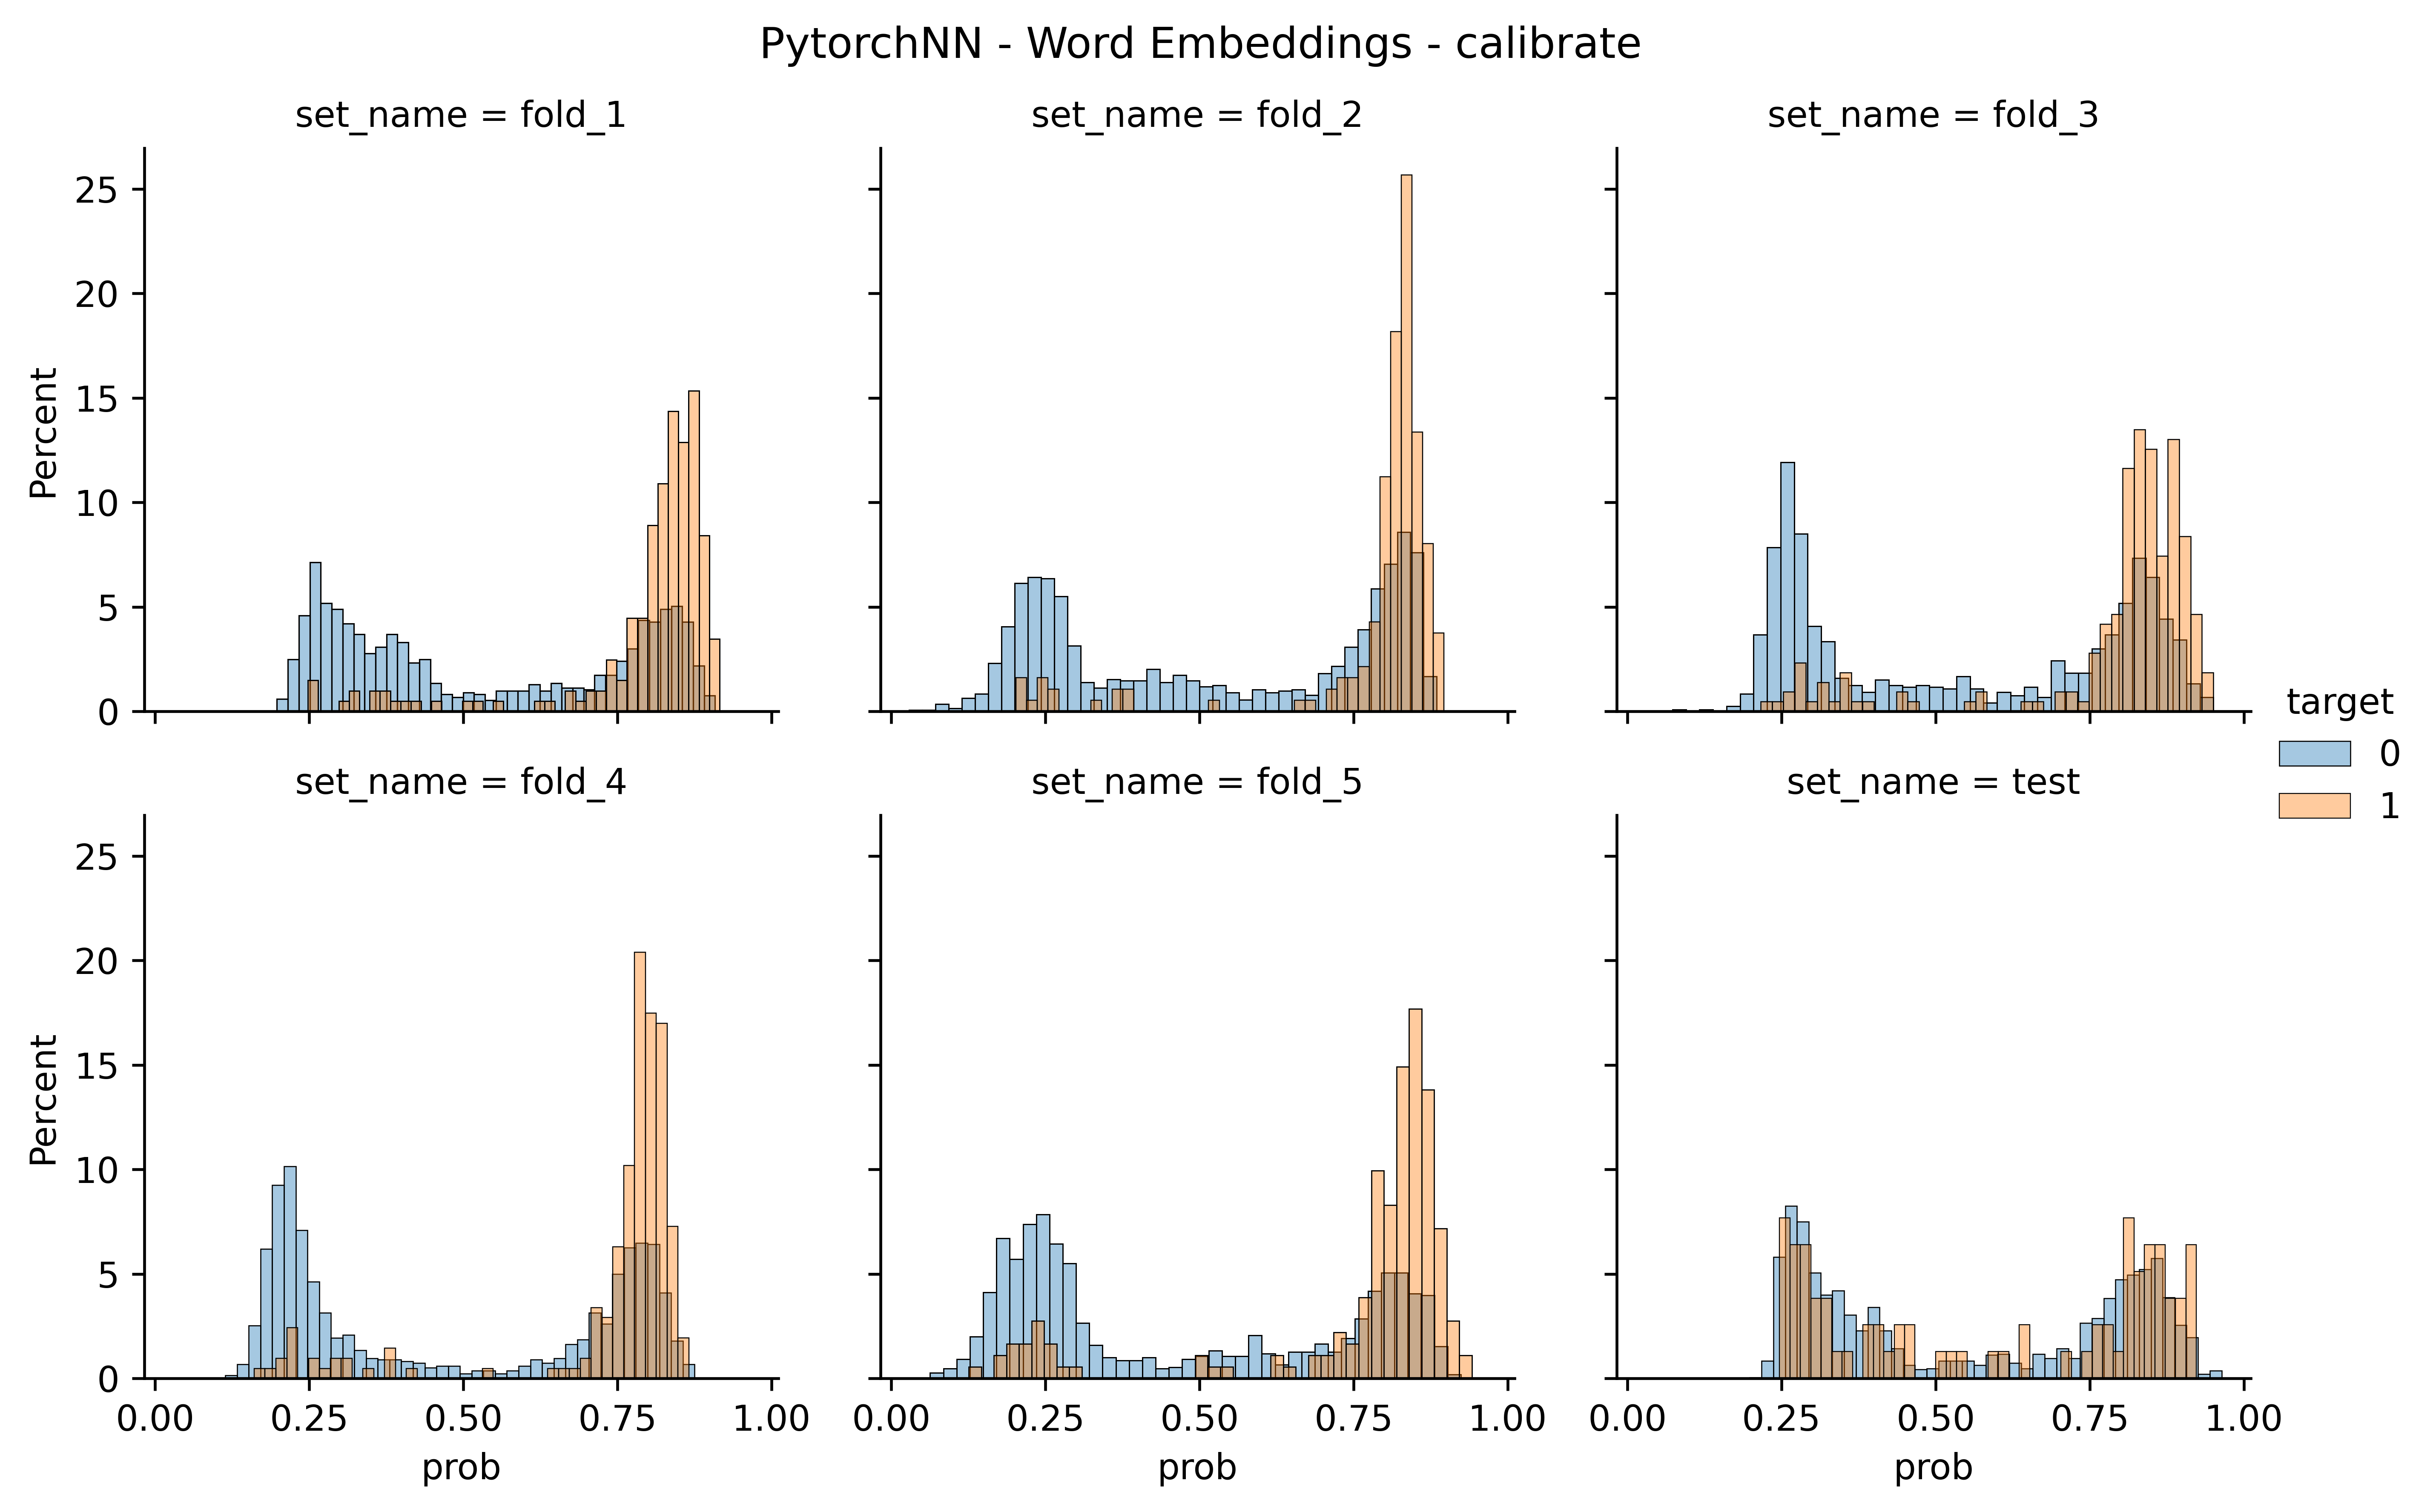
\includegraphics[width=\linewidth]{figures/results/word_embeddings/nn/calibrate/calibrate__distplot.png}
%     \end{subfigure}
%     \caption{Word embeddings calibrate}
% \end{figure}
% 
% \begin{figure}
%     \centering
%     \begin{subfigure}[b]{0.83\textwidth}
%     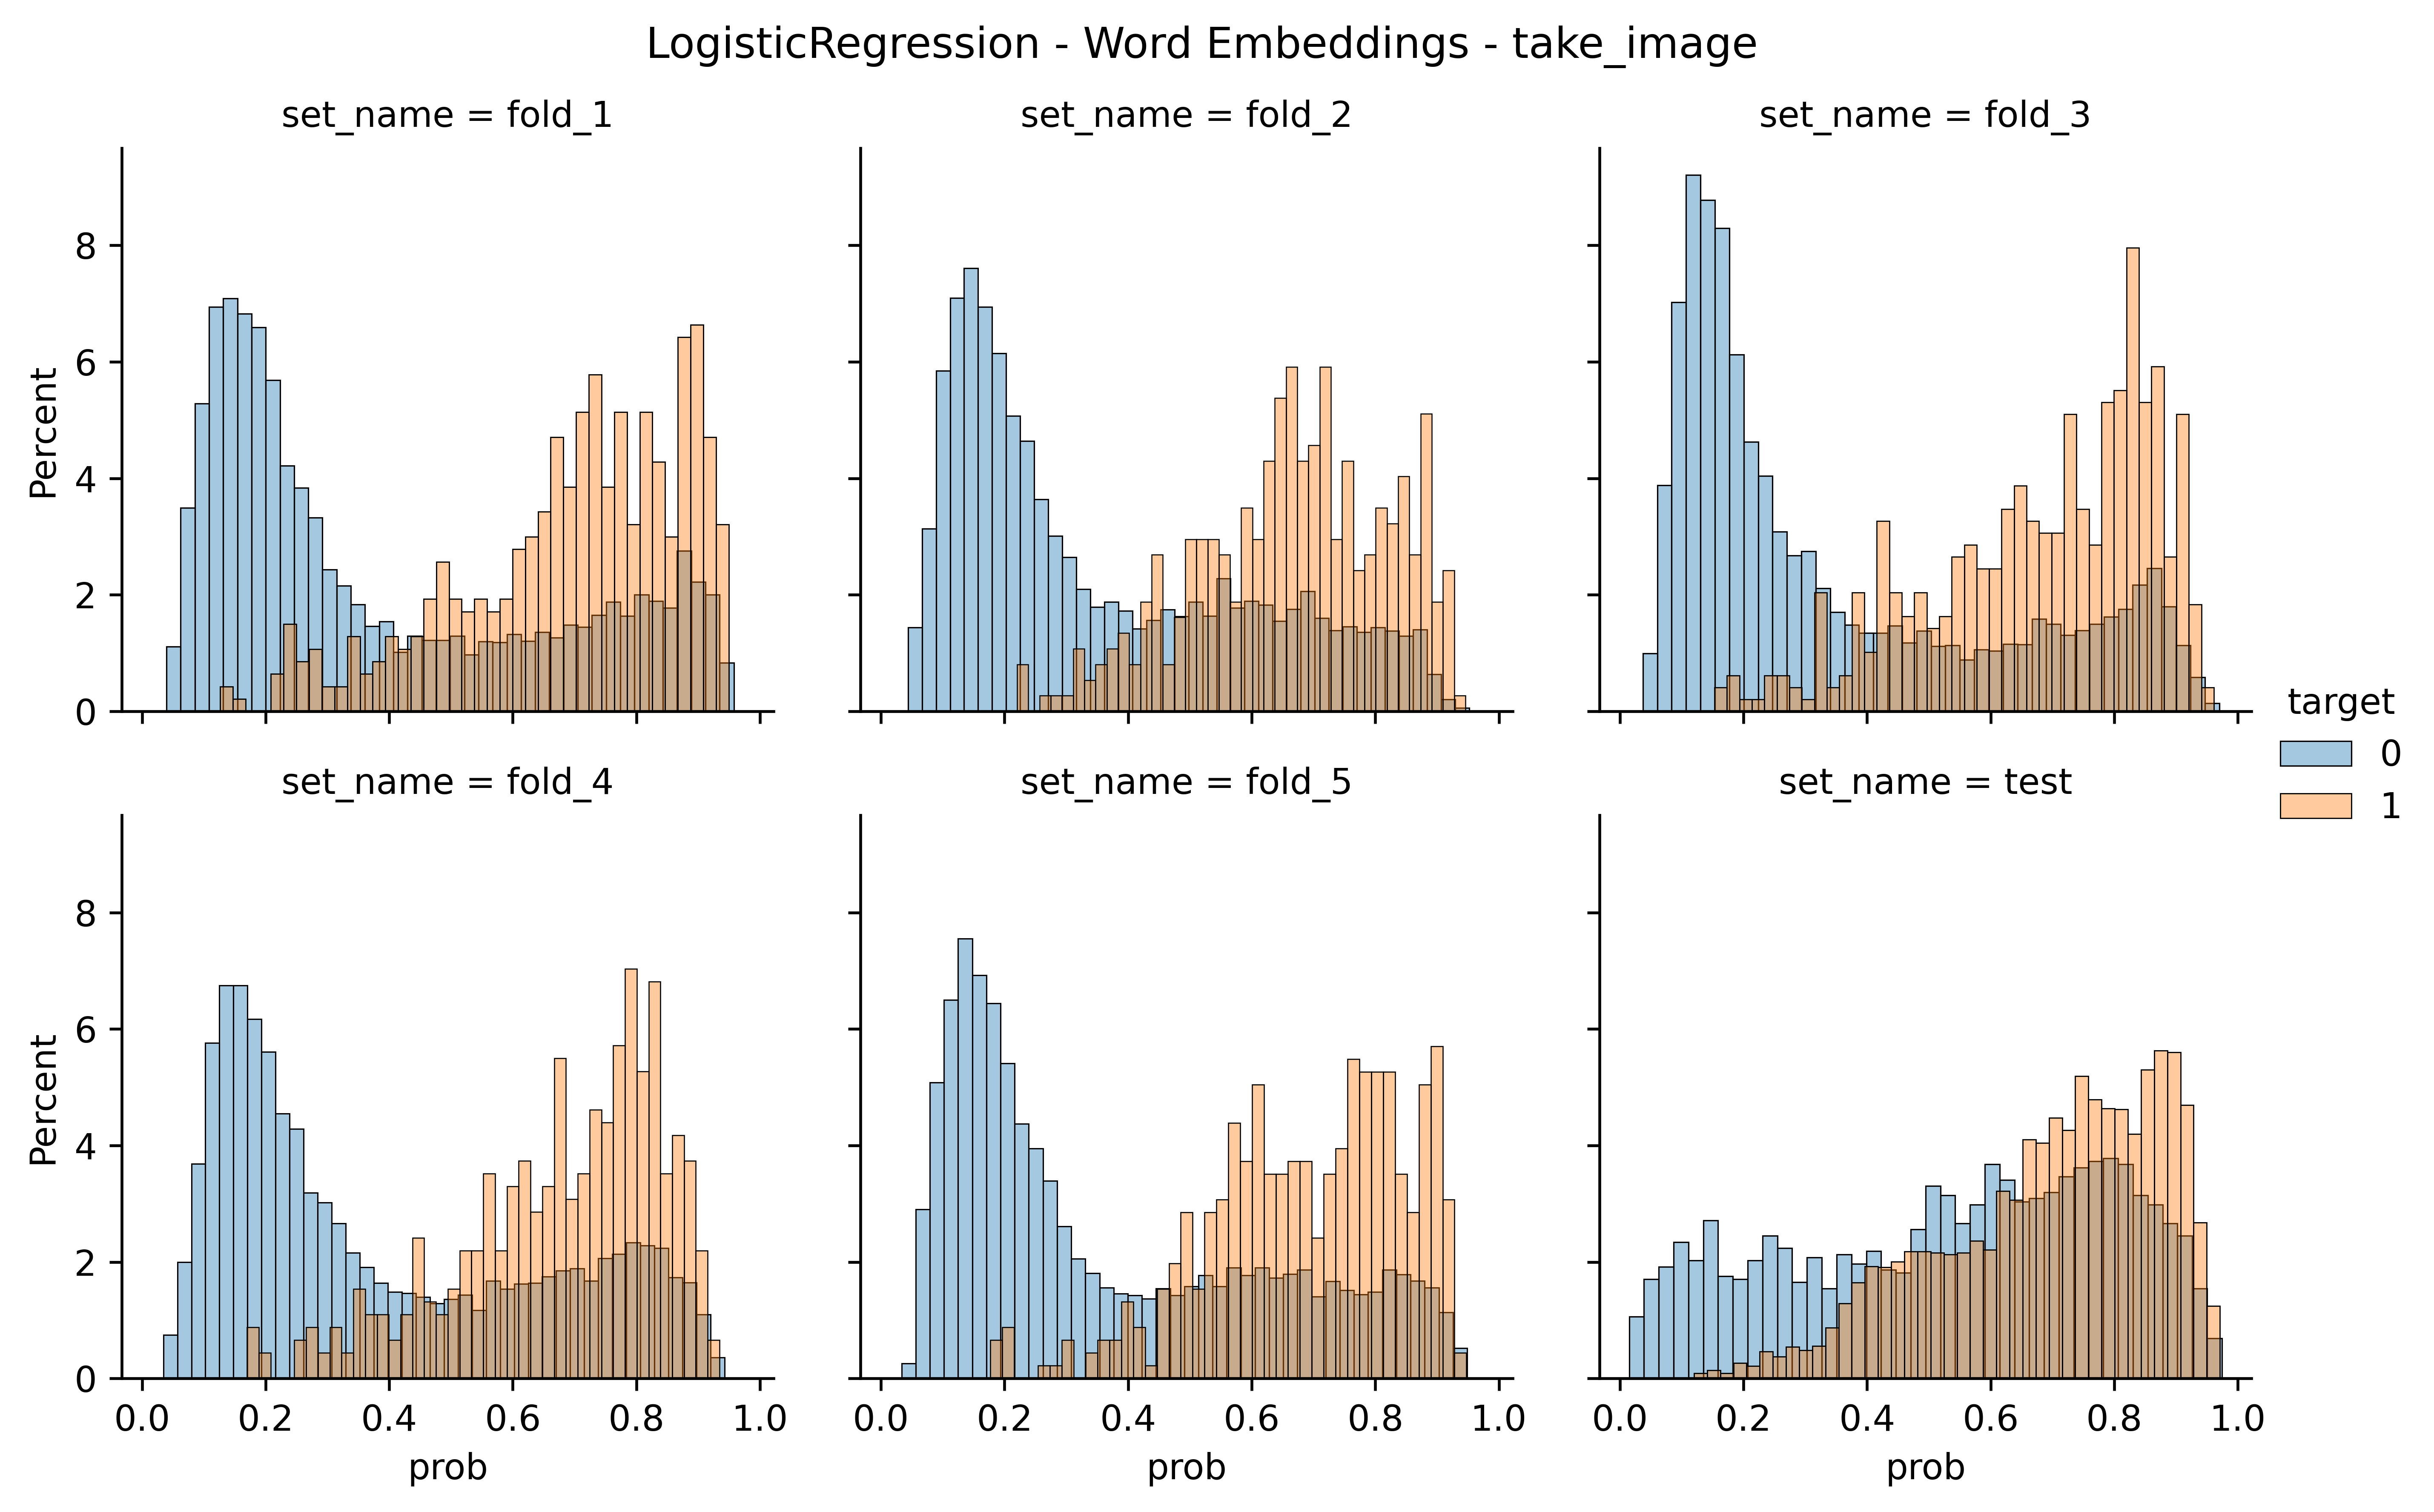
\includegraphics[width=\linewidth]{figures/results/word_embeddings/lgr/take_image/lgr__distplot.png}
%     \end{subfigure}
%     \hfill
%     \centering
%     \begin{subfigure}[b]{0.83\textwidth}
%         \centering
%         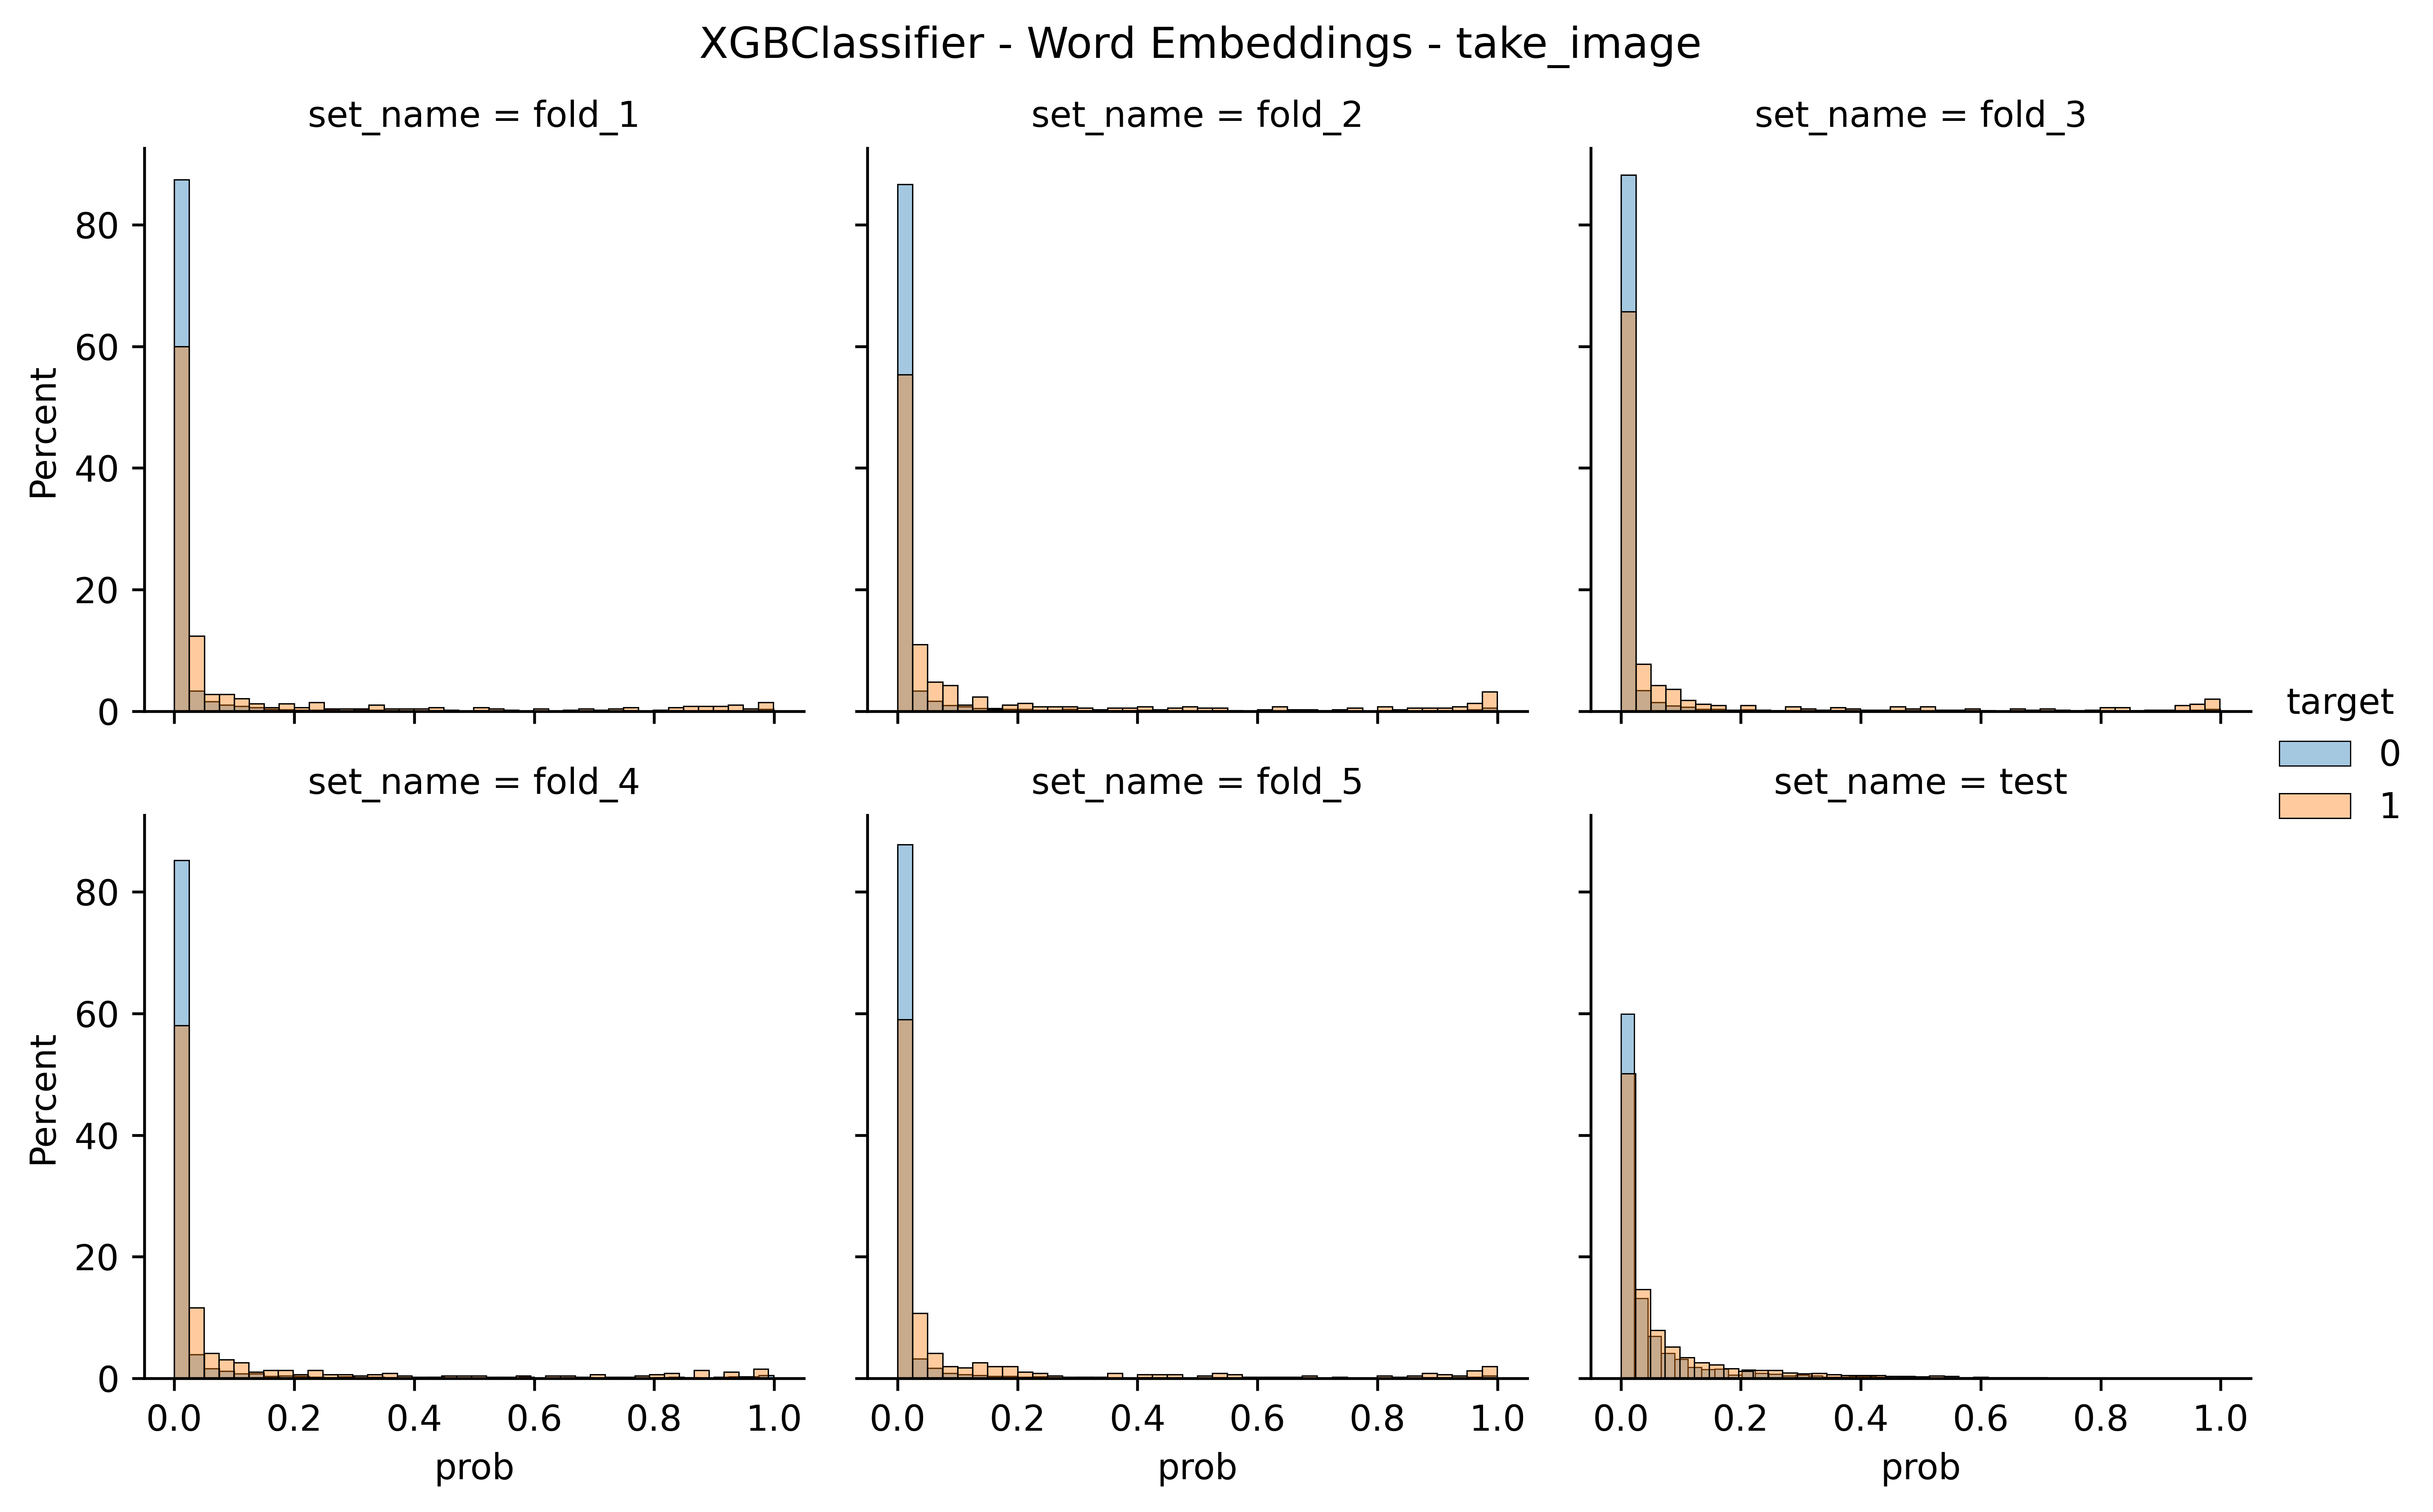
\includegraphics[width=\linewidth]{figures/results/word_embeddings/xgboost/take_image/take_image__distplot.png}
%     \end{subfigure}
%     \hfill
%     \centering
%     \begin{subfigure}[b]{0.83\textwidth}
%         \centering
%         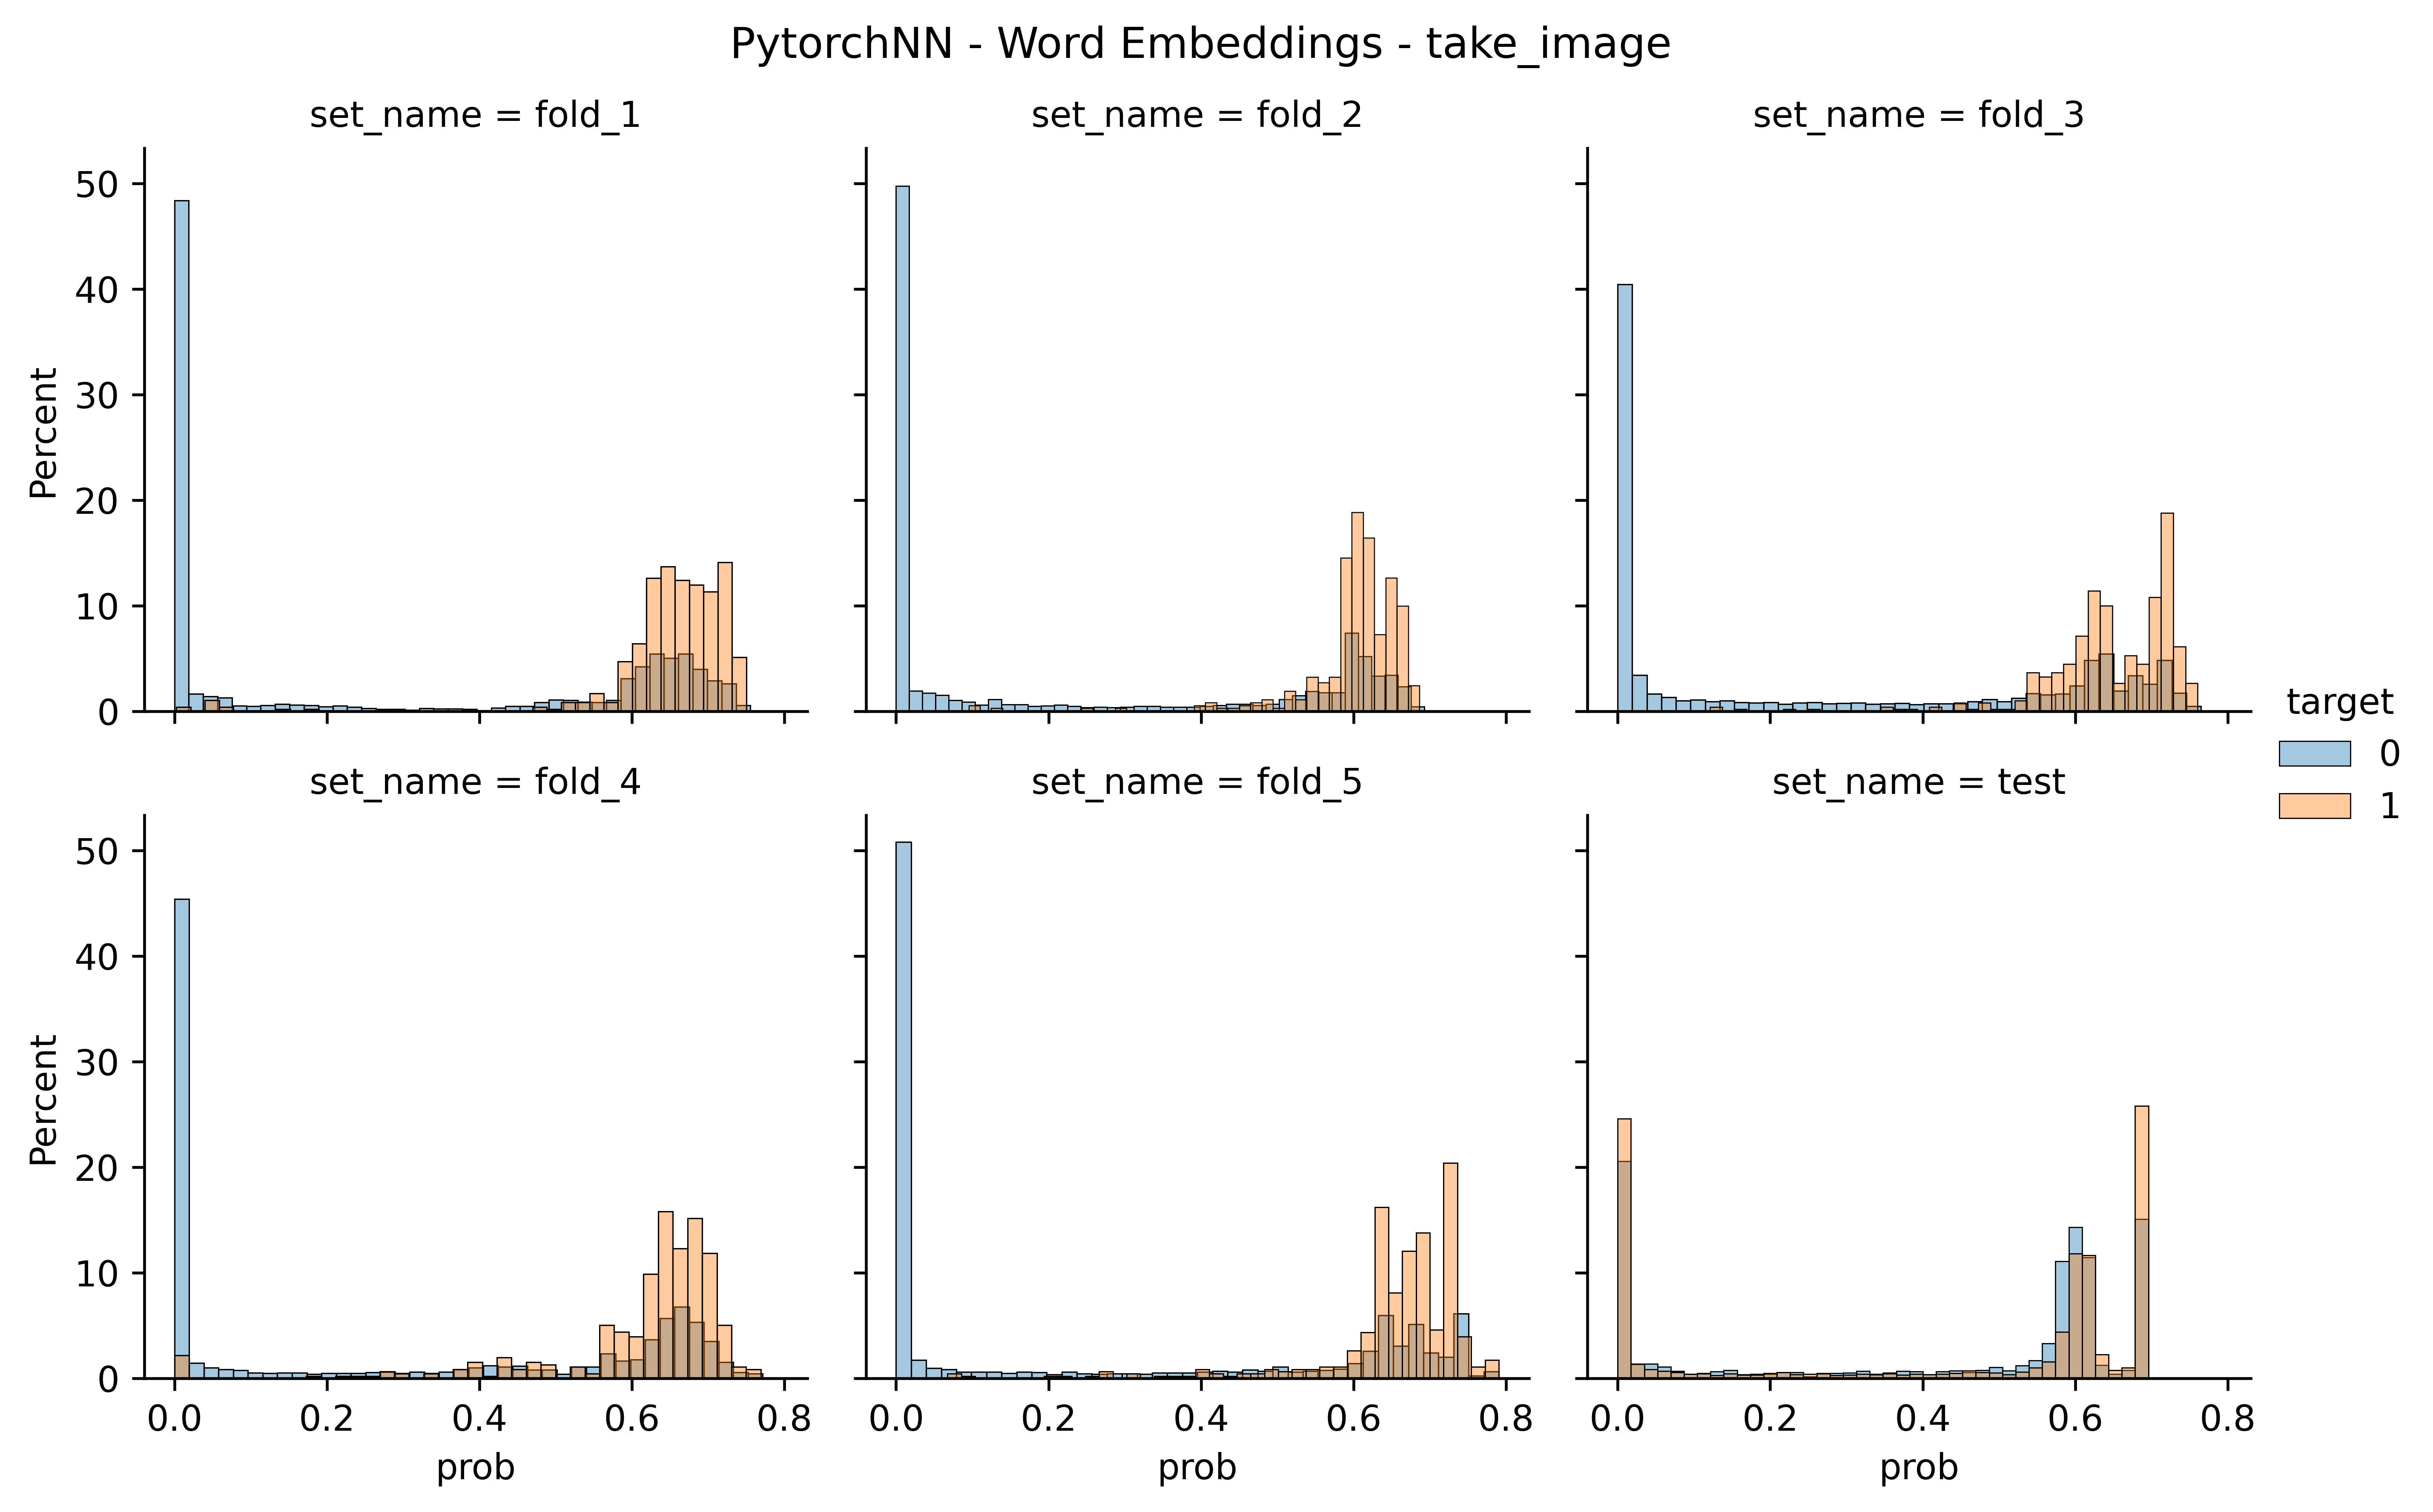
\includegraphics[width=\linewidth]{figures/results/word_embeddings/nn/take_image/take_image__distplot (1).png}
%     \end{subfigure}
%     \caption{Word embeddings take\_image}
% \end{figure}
% 
% \begin{figure}
%     \centering
%     \begin{subfigure}[b]{0.83\textwidth}
%     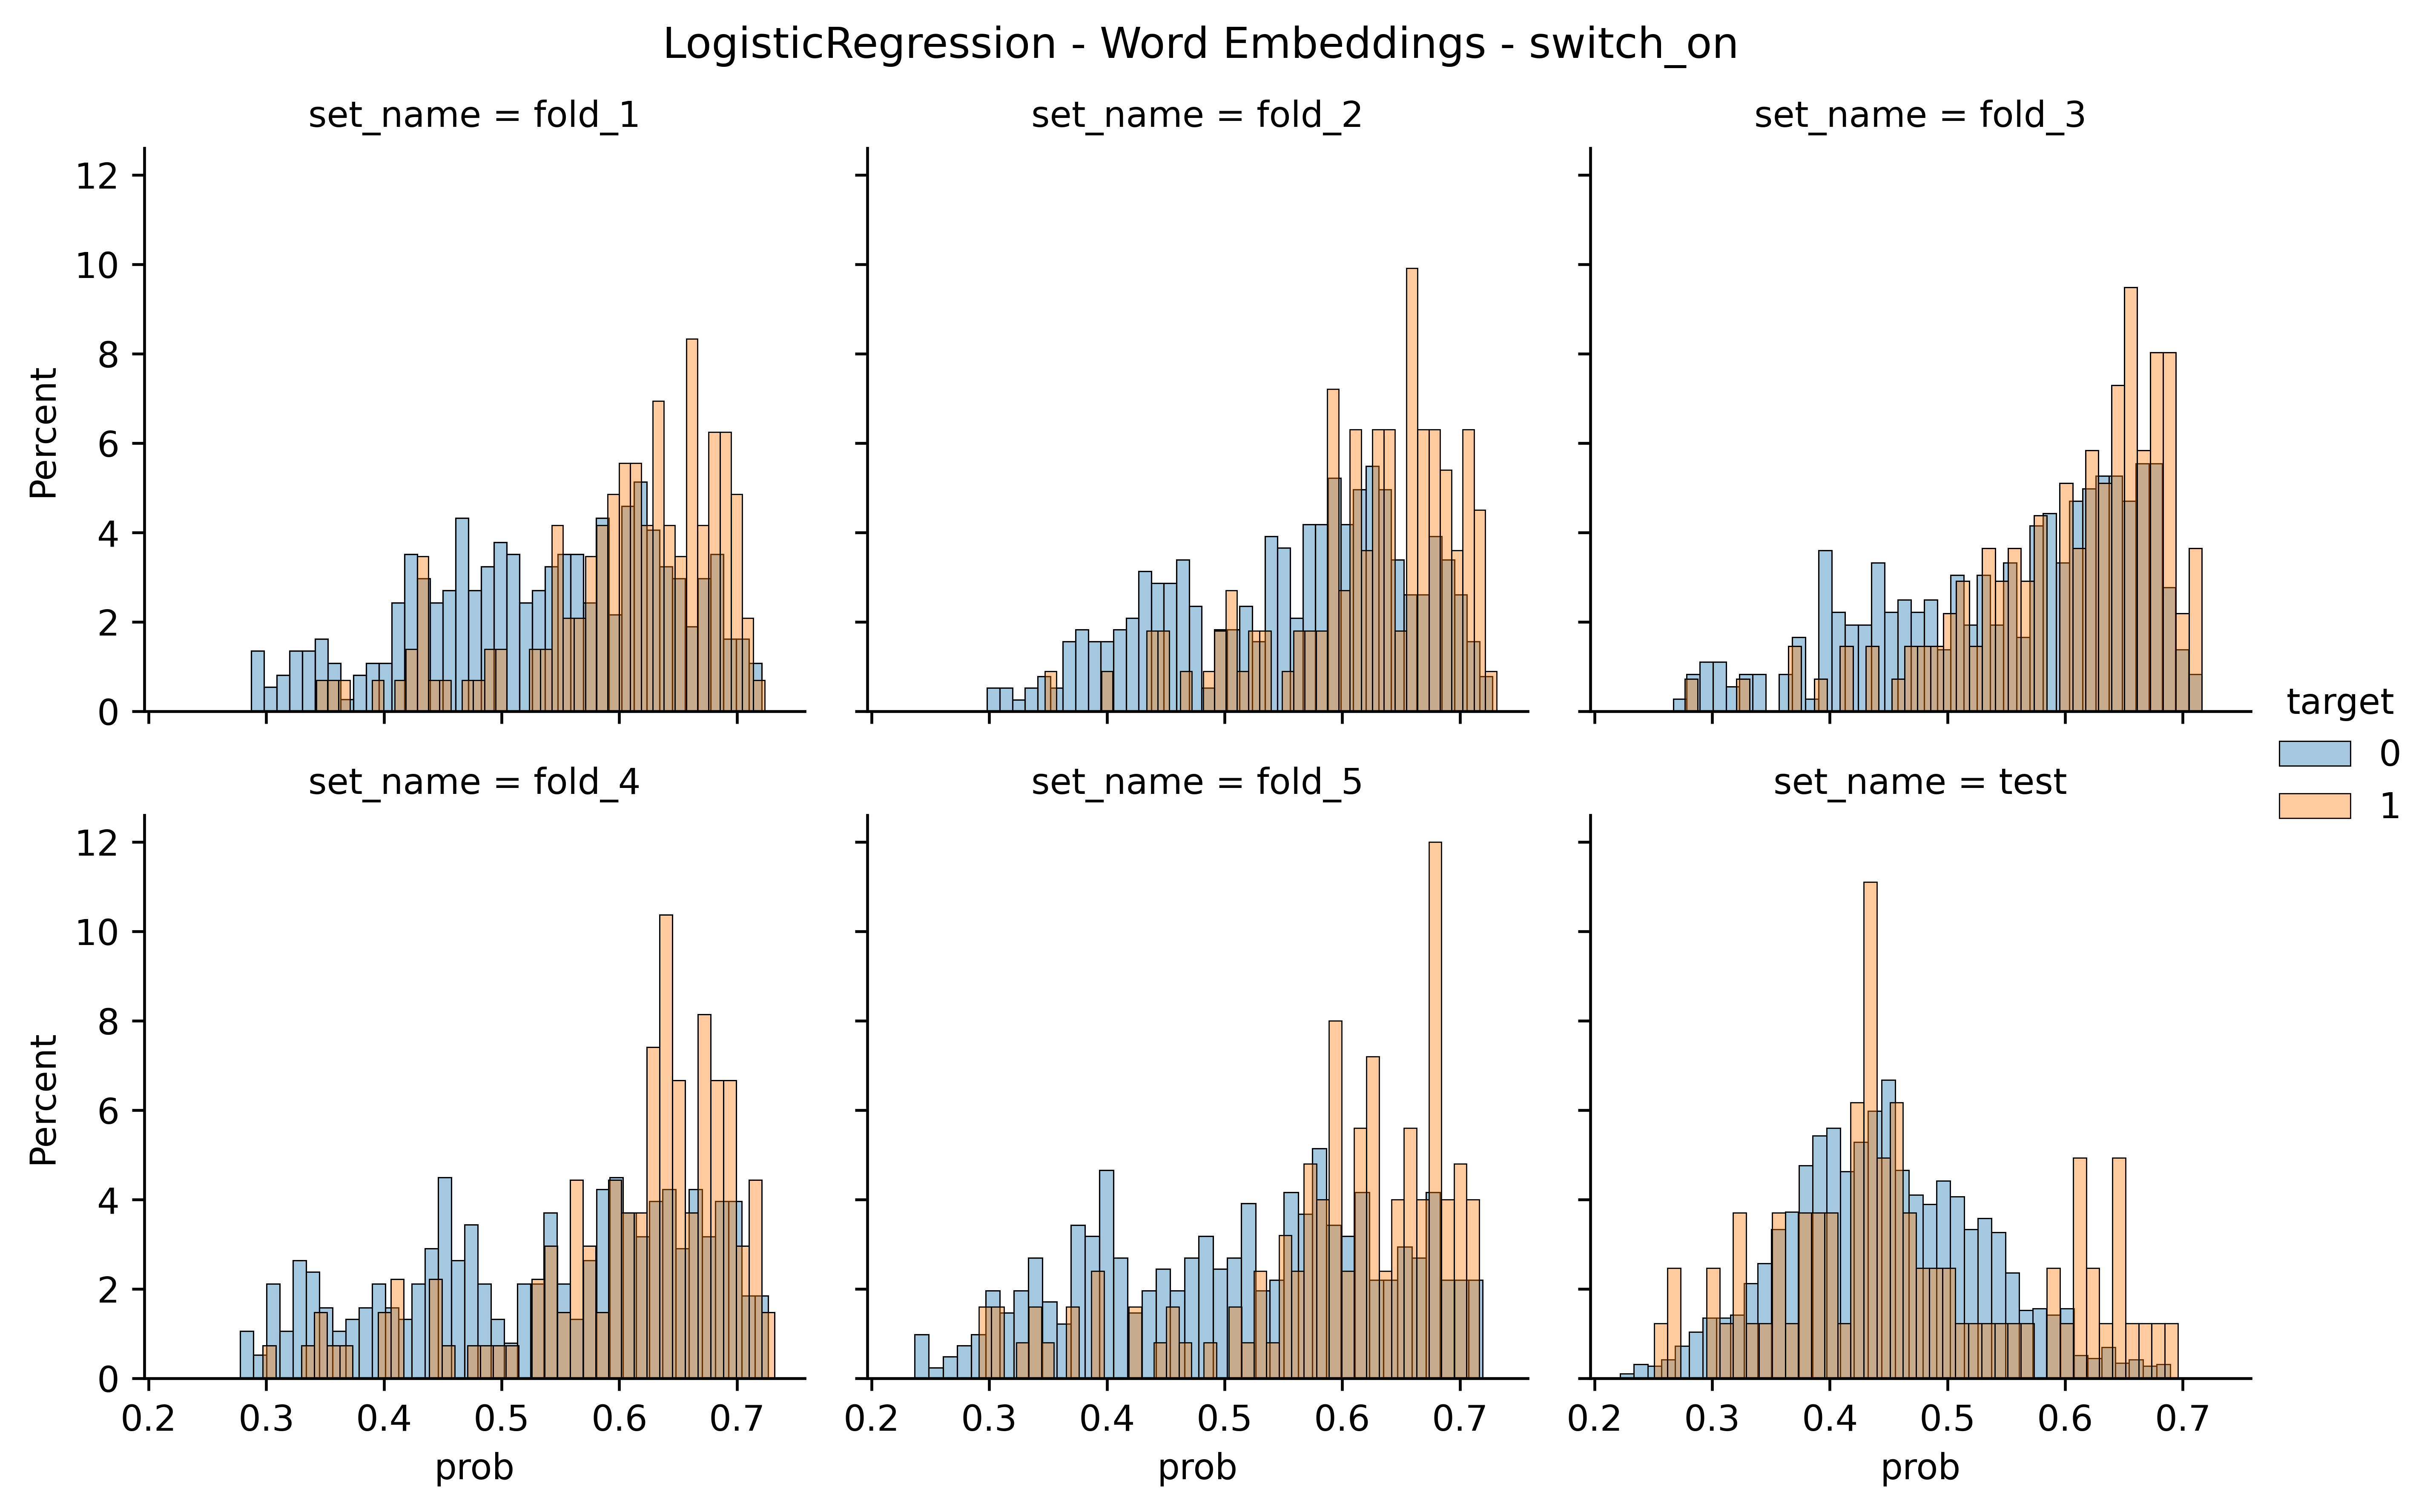
\includegraphics[width=\linewidth]{figures/results/word_embeddings/lgr/switch_on/switch_on__distplot.png}
%     \end{subfigure}
%     \hfill
%     \centering
%     \begin{subfigure}[b]{0.83\textwidth}
%         \centering
%         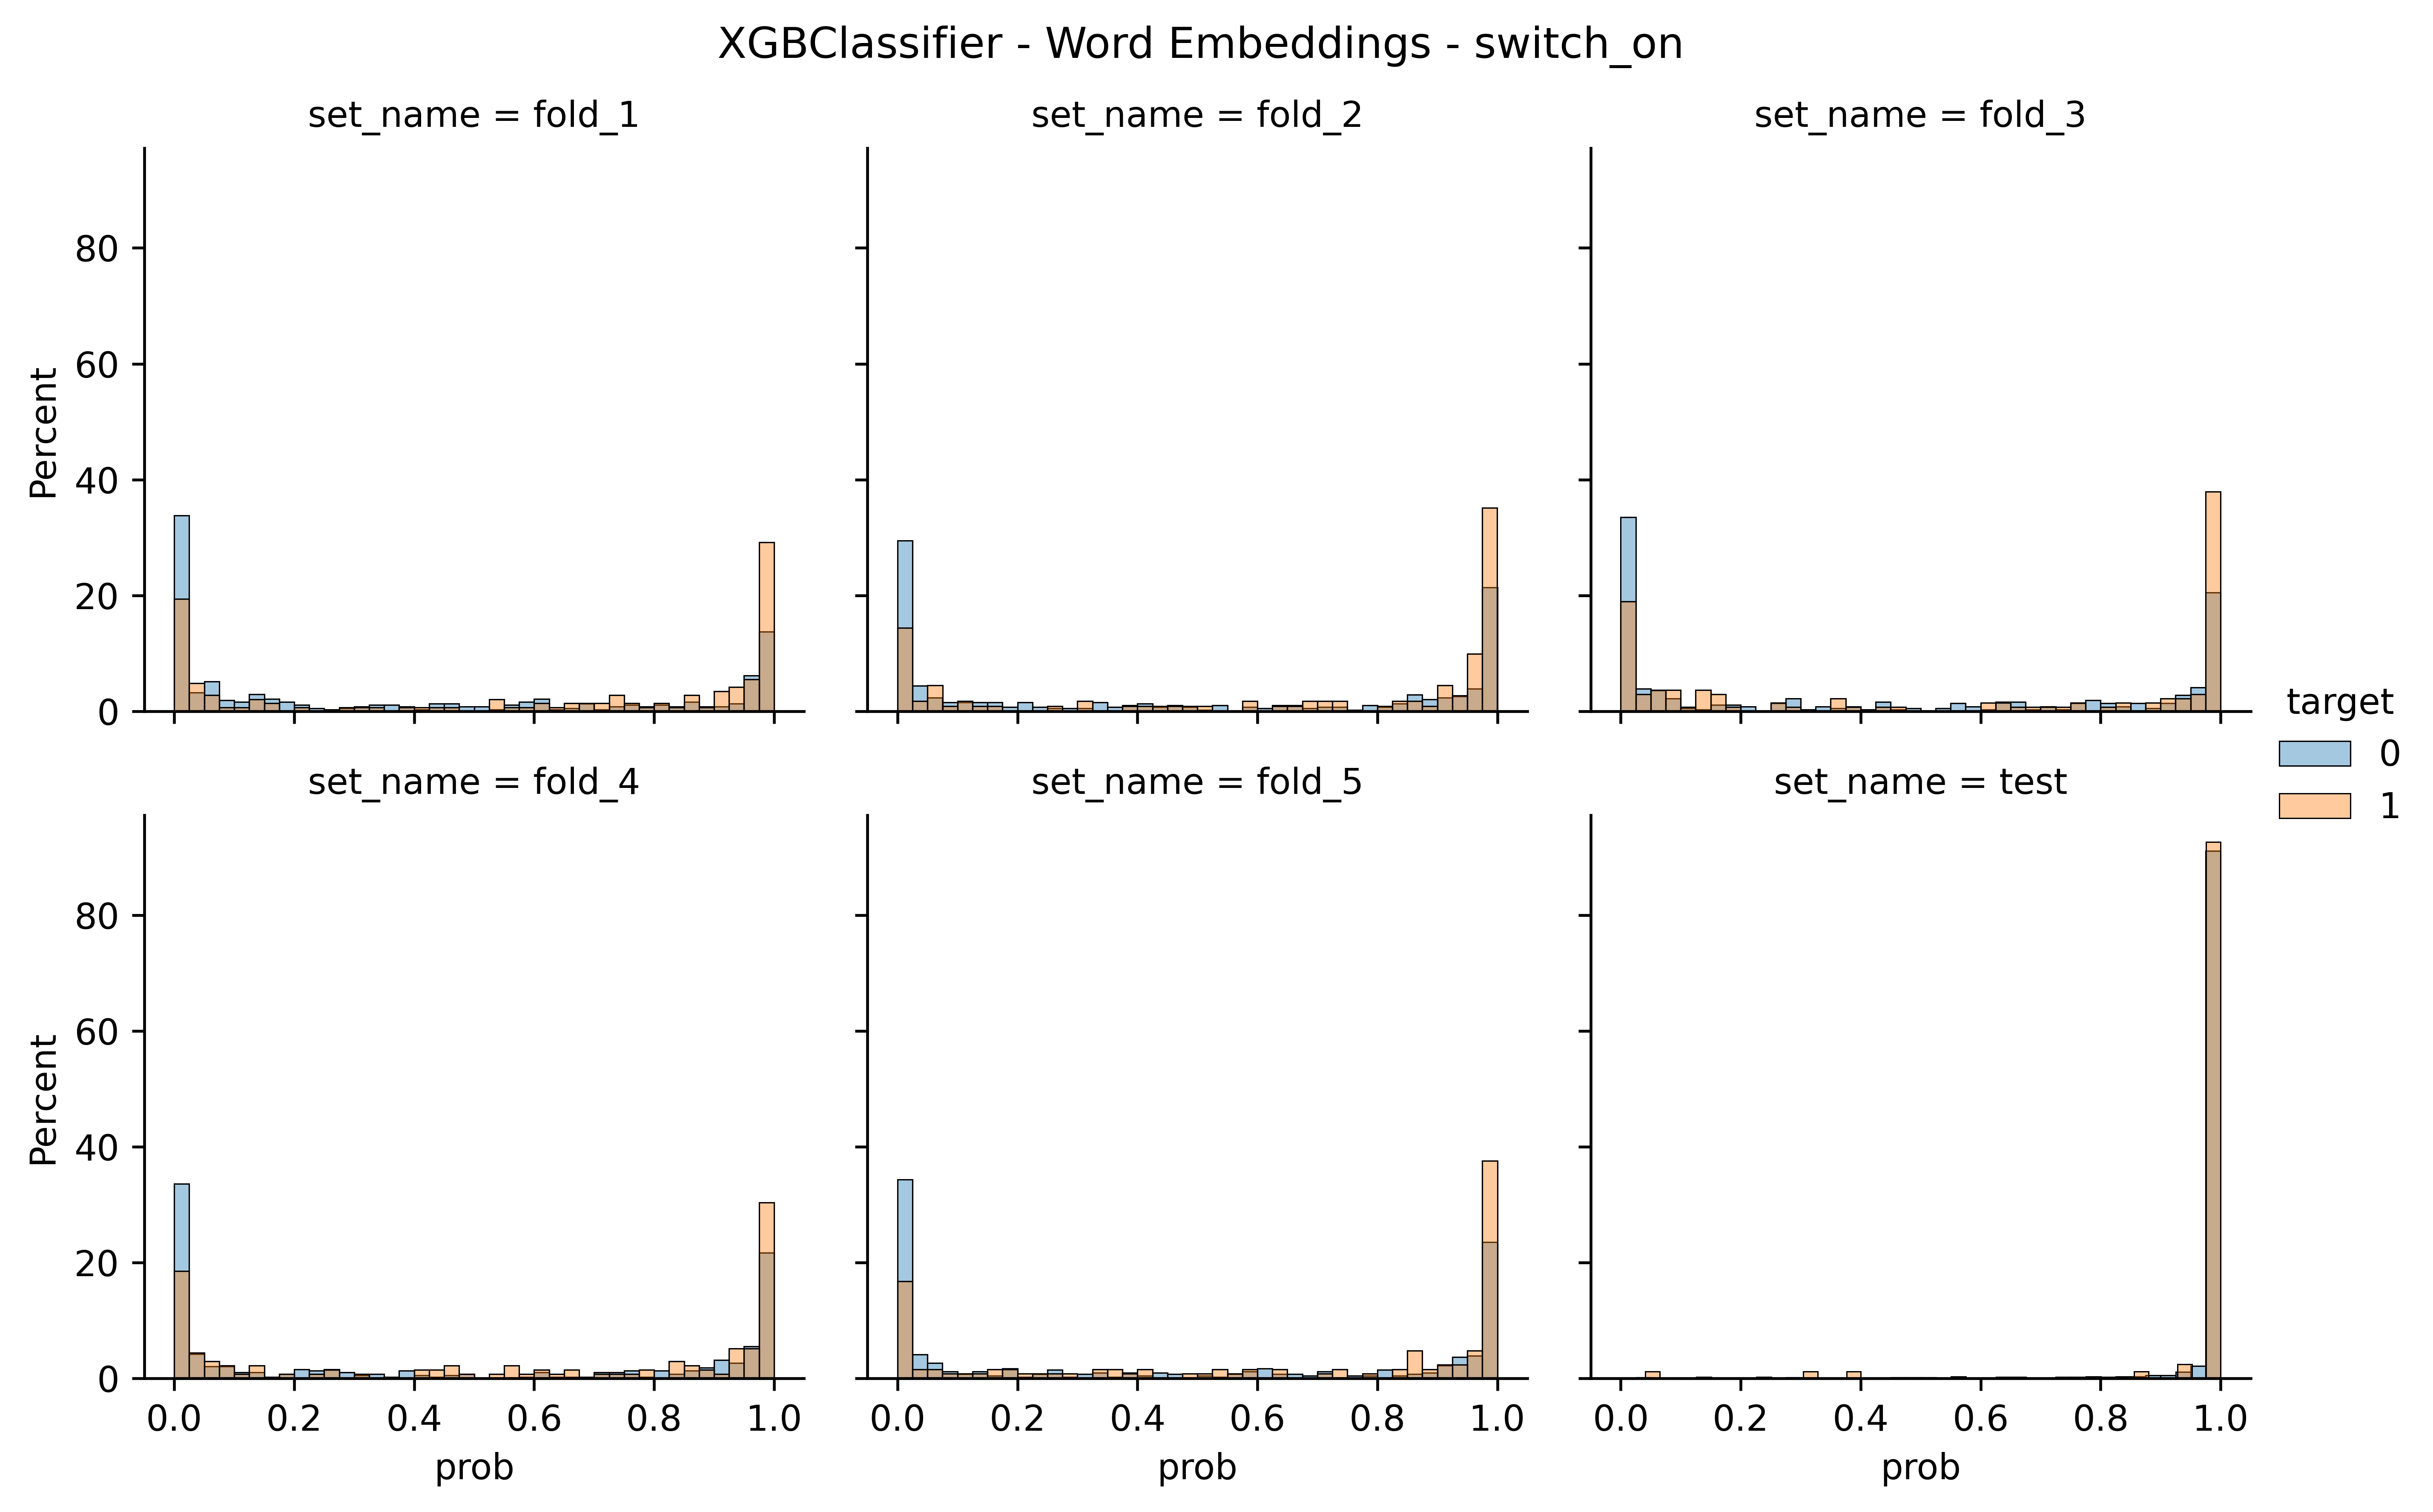
\includegraphics[width=\linewidth]{figures/results/word_embeddings/xgboost/switch_on/xgb__distplot.png}
%     \end{subfigure}
%     \hfill
%     \centering
%     \begin{subfigure}[b]{0.83\textwidth}
%         \centering
%         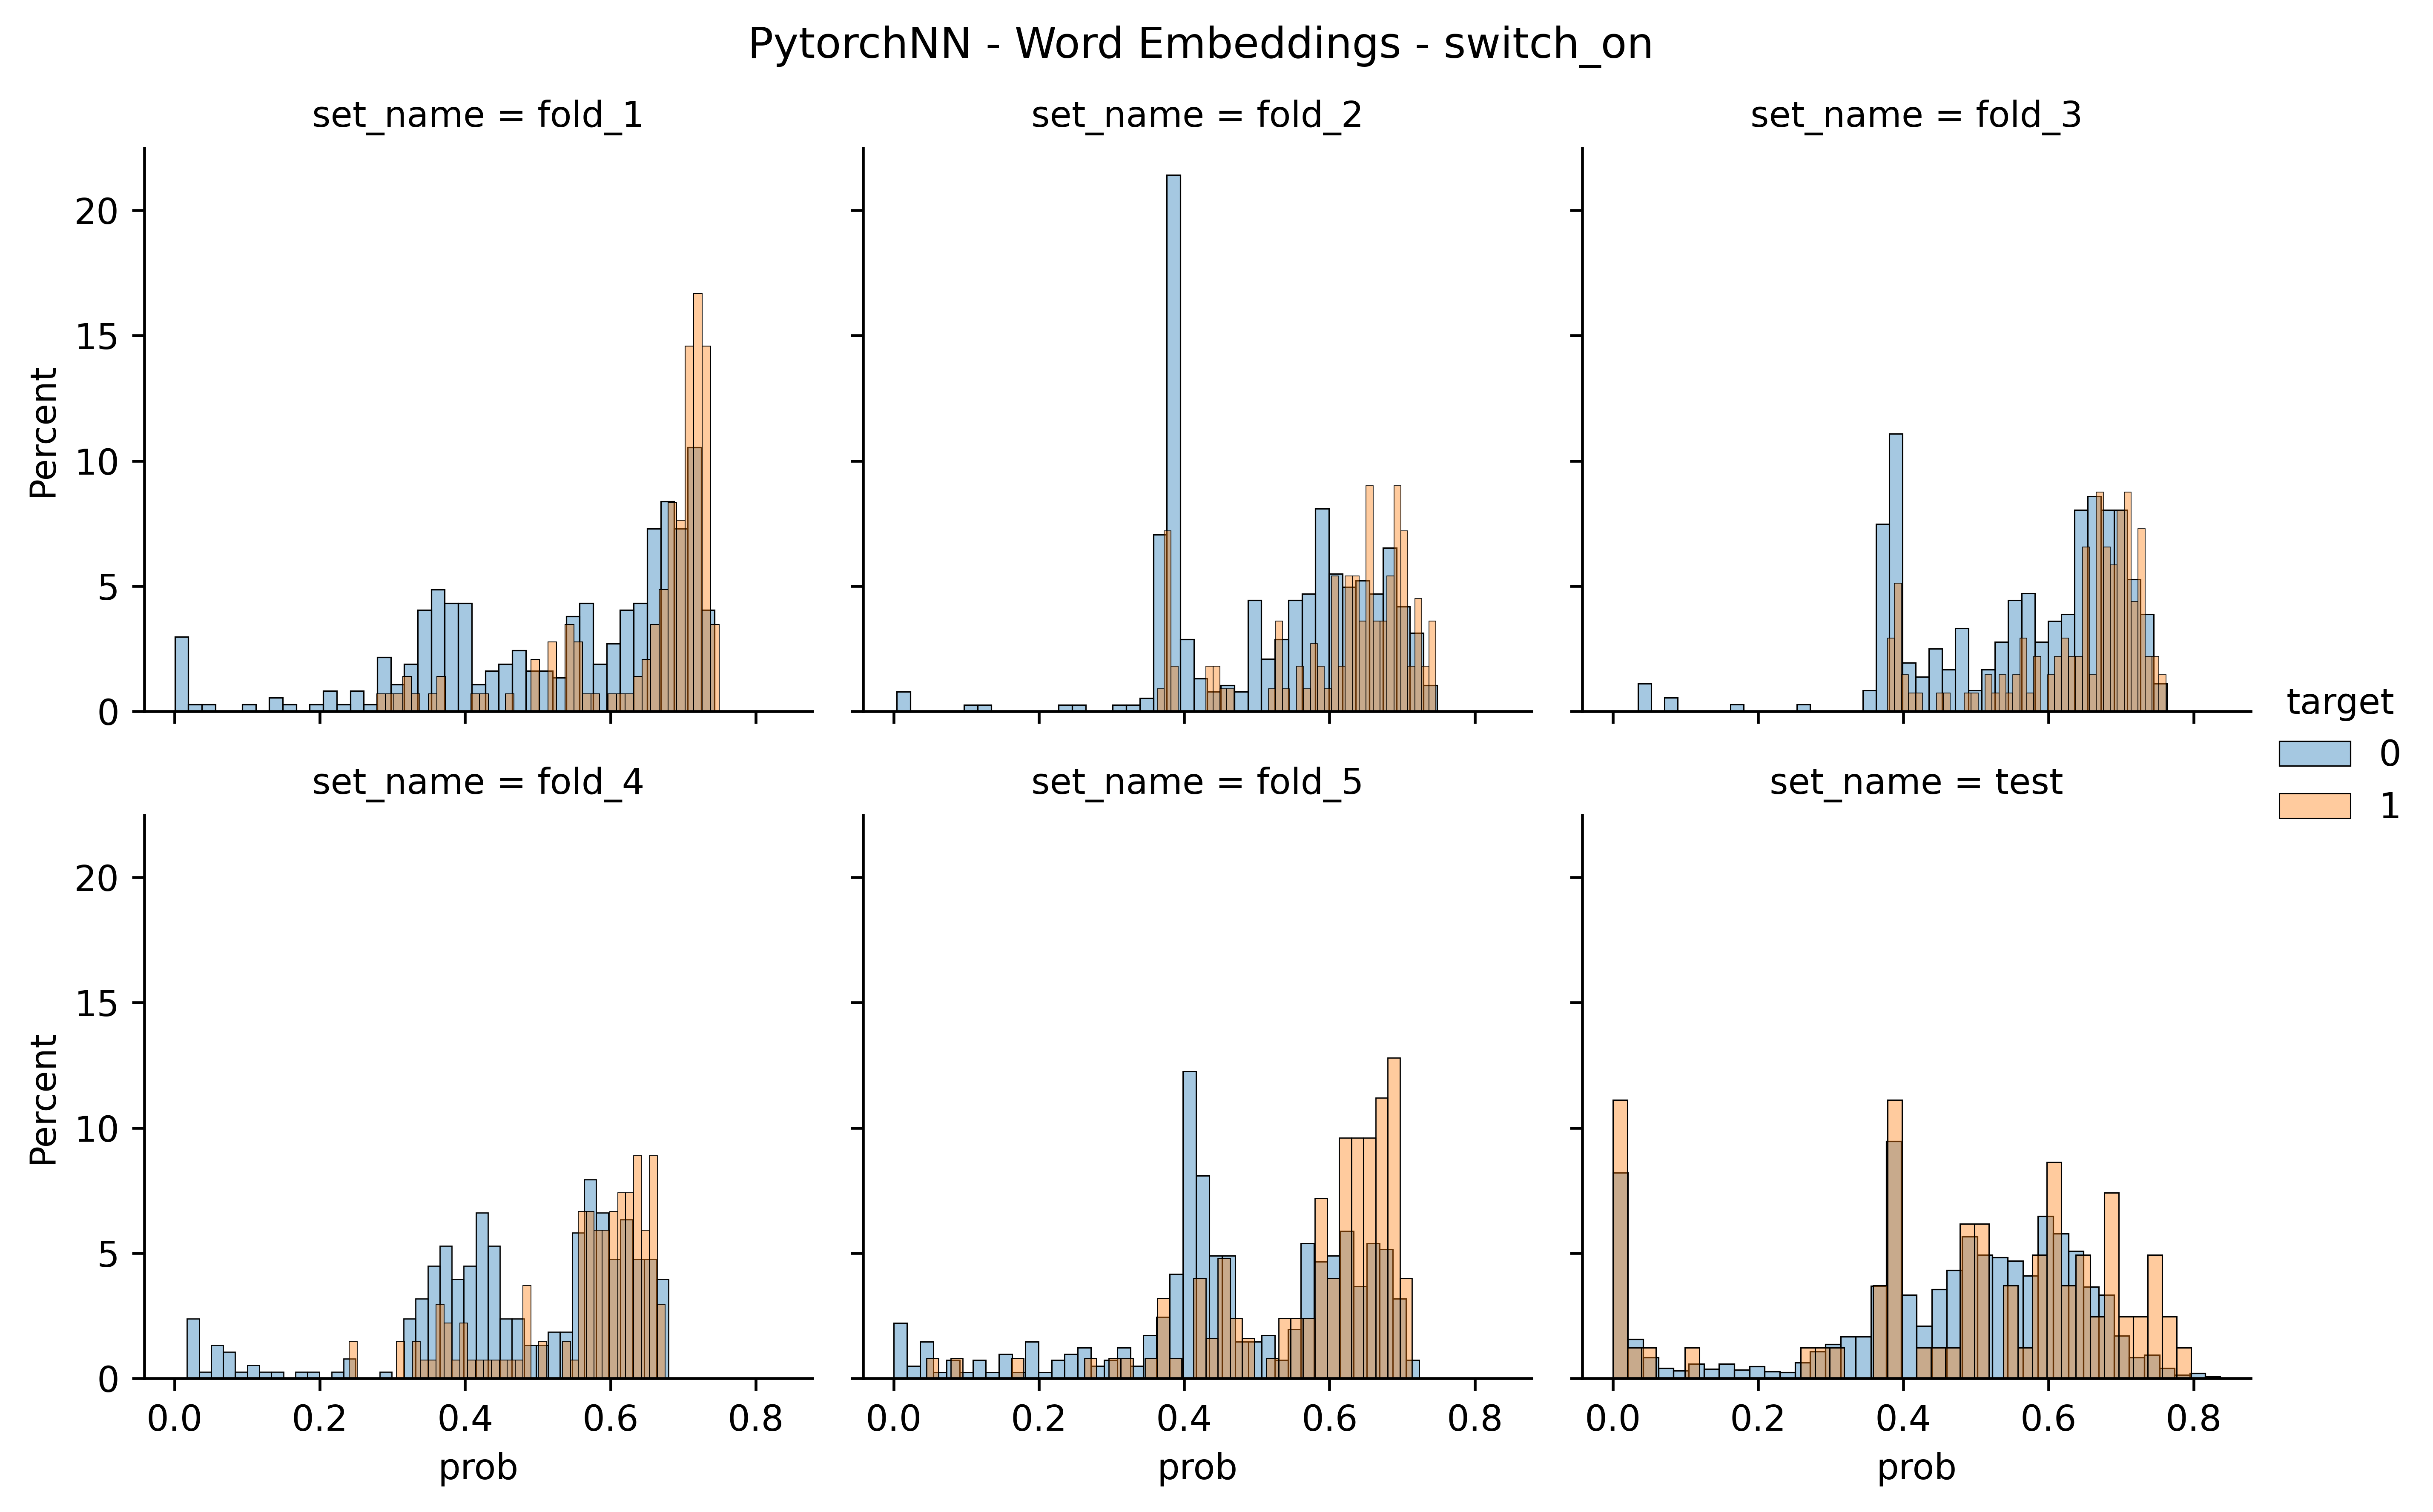
\includegraphics[width=\linewidth]{figures/results/word_embeddings/nn/switch_on/switch_on__distplot (1).png}
%     \end{subfigure}
%     \caption{Word embeddings switch\_on}
% \end{figure}
% 
% 
% \begin{figure}
%     \begin{subfigure}[b]{\textwidth}
%         \centering
%         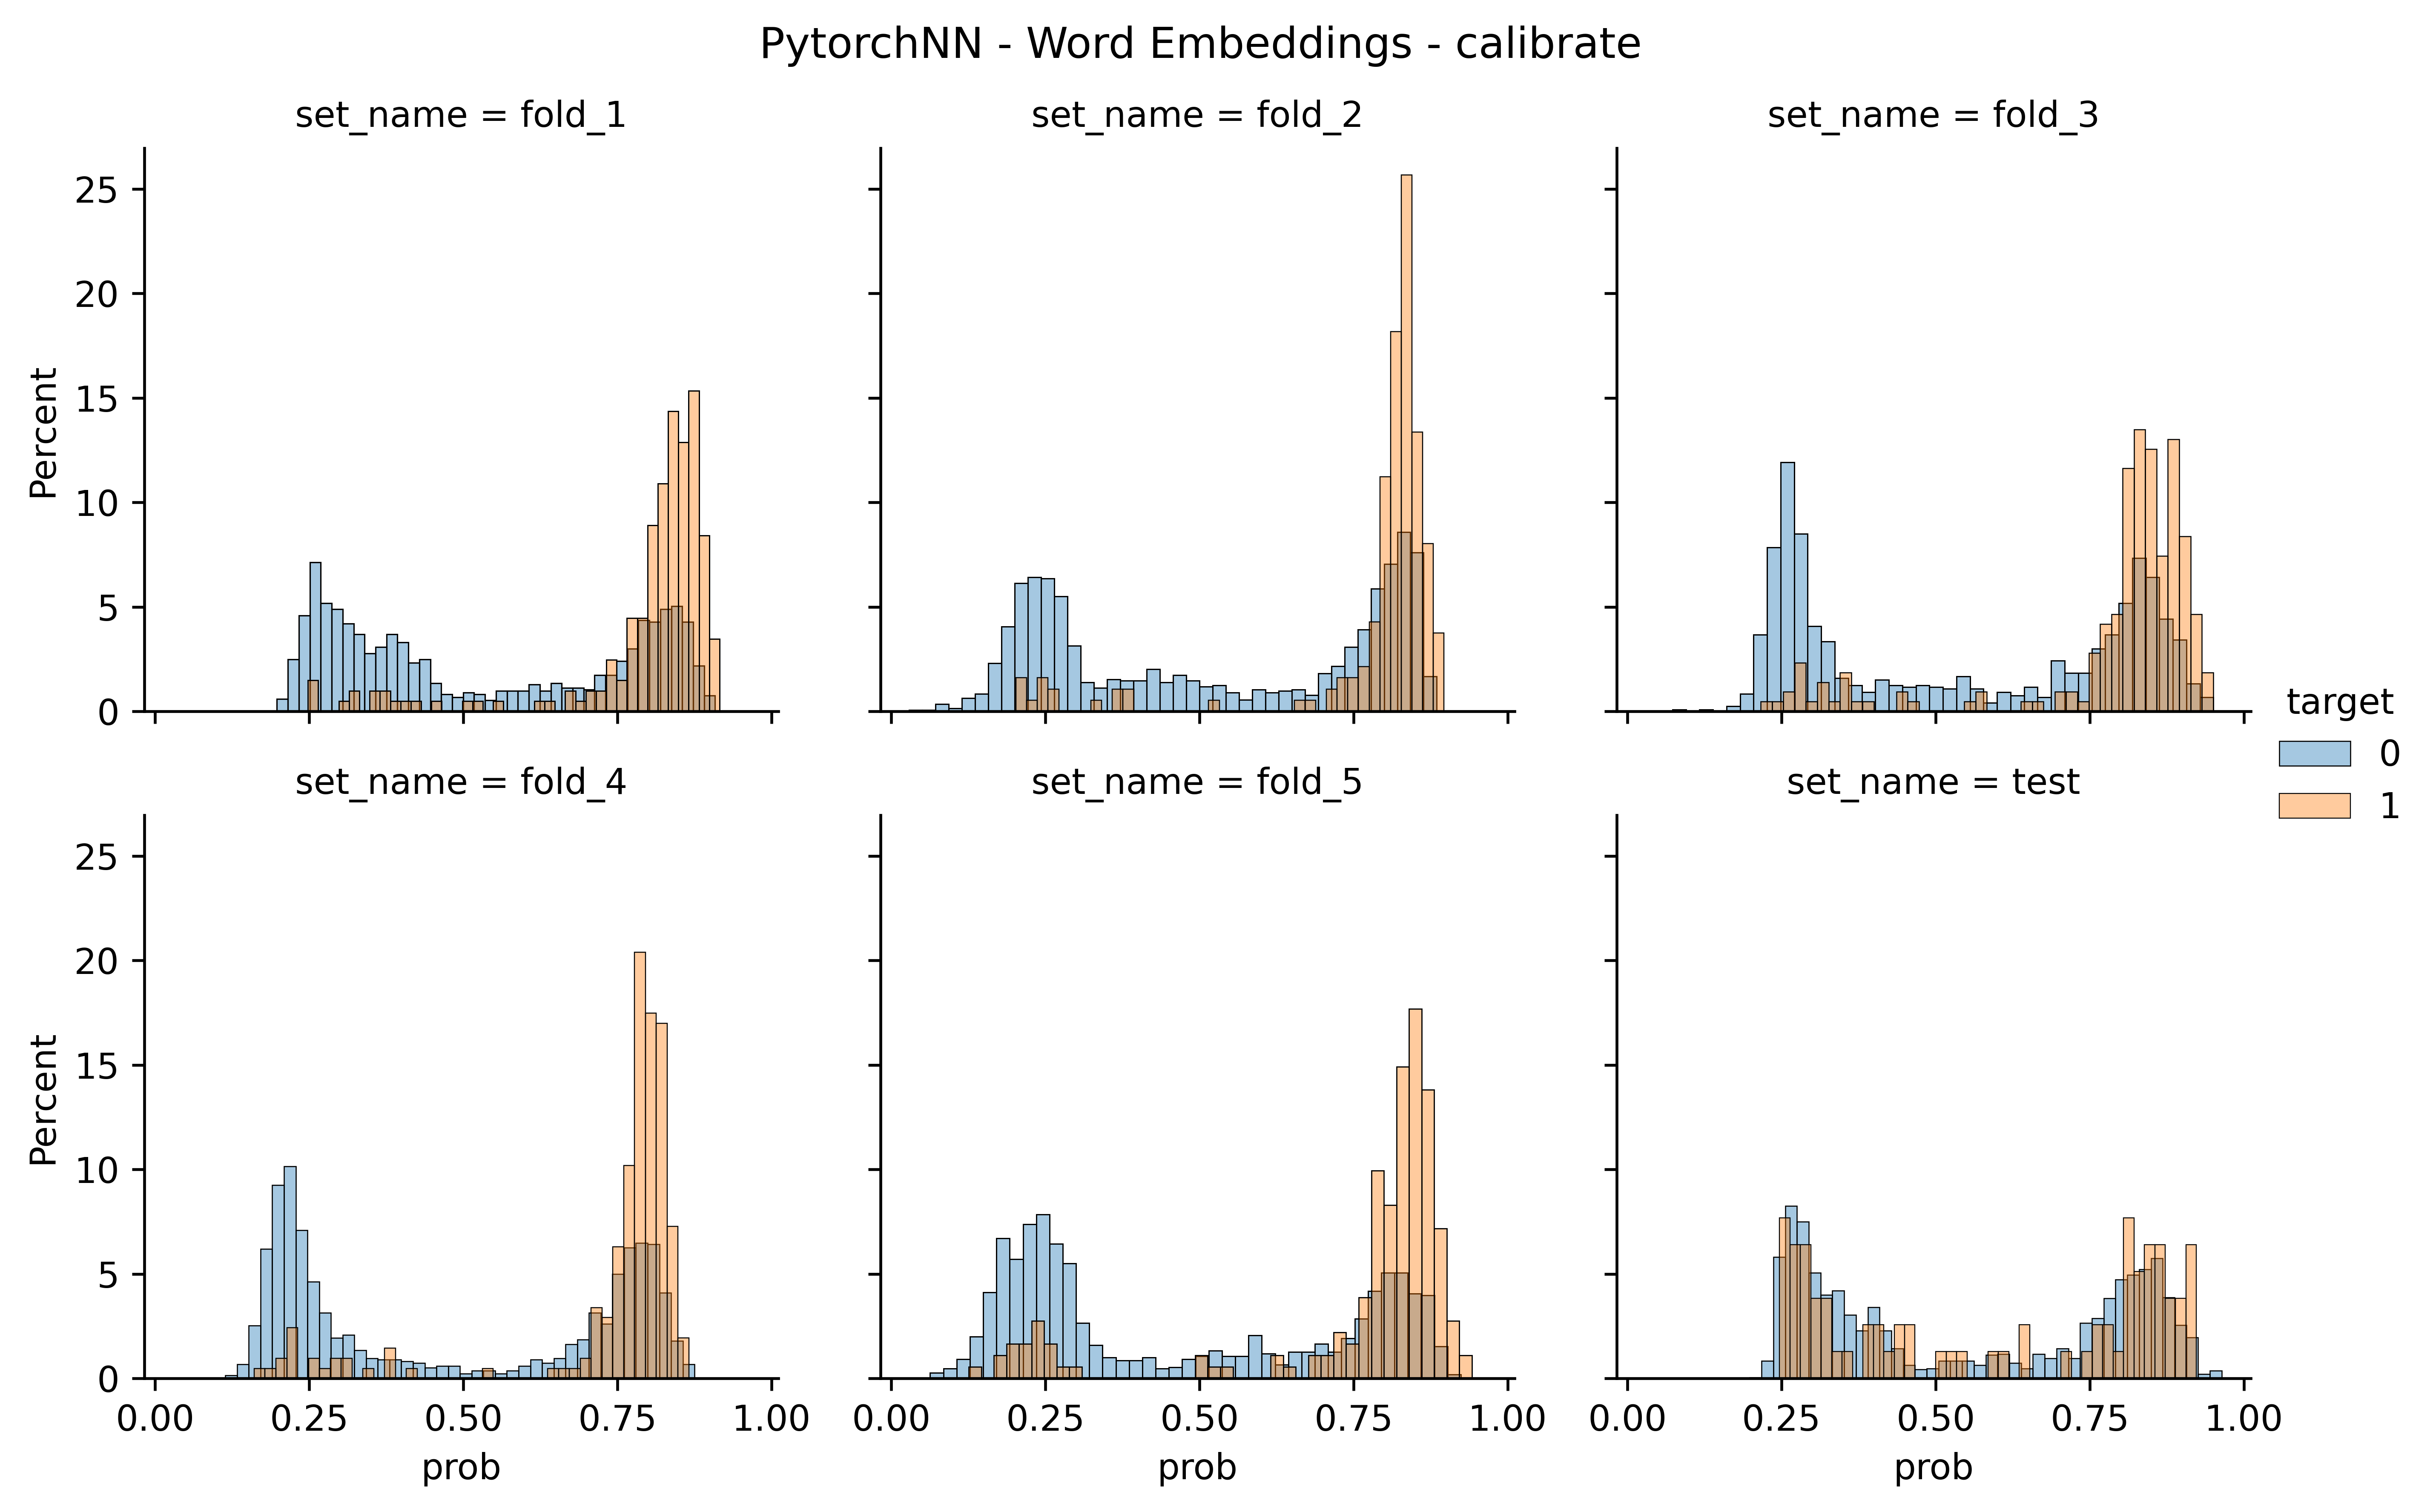
\includegraphics[width=\linewidth]{figures/results/word_embeddings/nn/calibrate/calibrate__distplot.png}
%         \caption{Distribución de predicciones en validación cruzada y el conjunto de test.}
%         \label{fig:my_label}
%     \end{subfigure}
%     \hfill
%     \begin{subfigure}[b]{\textwidth}
%     \minipage{0.32\textwidth}
%       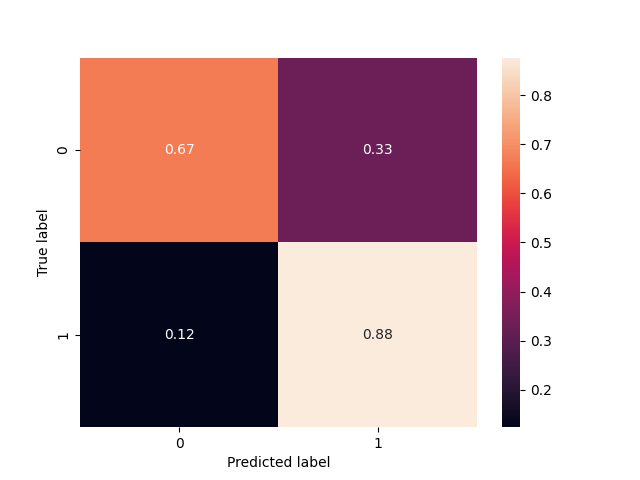
\includegraphics[width=\linewidth]{figures/results/word_embeddings/nn/calibrate/calibrate_set_1_confusion_matrix_percent.png}
%     \endminipage\hfill
%     \minipage{0.32\textwidth}
%       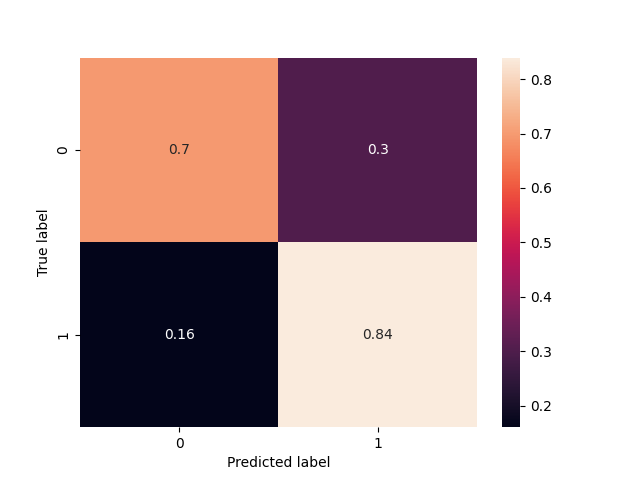
\includegraphics[width=\linewidth]{figures/results/word_embeddings/nn/calibrate/calibrate_set_2_confusion_matrix_percent.png}
%     \endminipage\hfill \minipage{0.32\textwidth}%
%       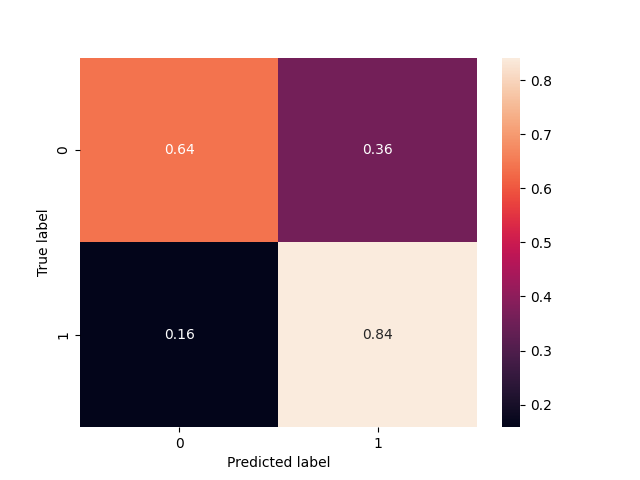
\includegraphics[width=\linewidth]{figures/results/word_embeddings/nn/calibrate/calibrate+_set_3_confusion_matrix_percent.png}
%     \endminipage
%     
%     \medskip
%     
%     \minipage{0.32\textwidth}
%       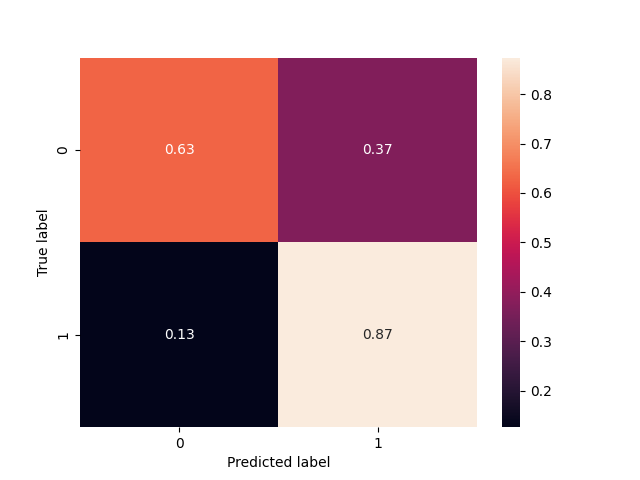
\includegraphics[width=\linewidth]{figures/results/word_embeddings/nn/calibrate/calibrate_set_4_confusion_matrix_percent.png}
%     \endminipage\hfill
%     \minipage{0.32\textwidth}
%     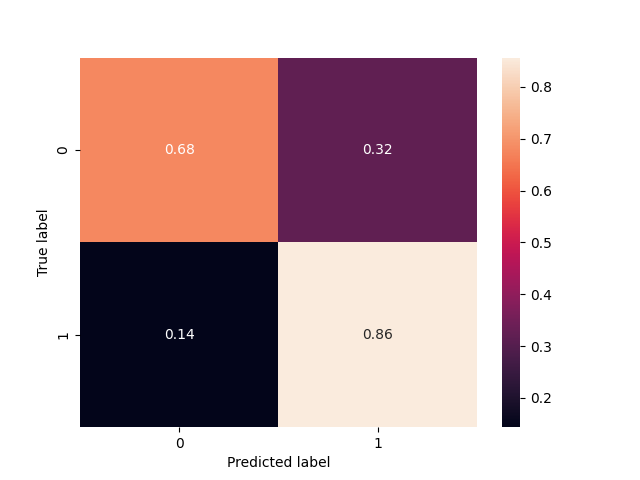
\includegraphics[width=\linewidth]{figures/results/word_embeddings/nn/calibrate/calibrate_set_5_confusion_matrix_percent.png}
%     \endminipage\hfill \minipage{0.32\textwidth}%
%     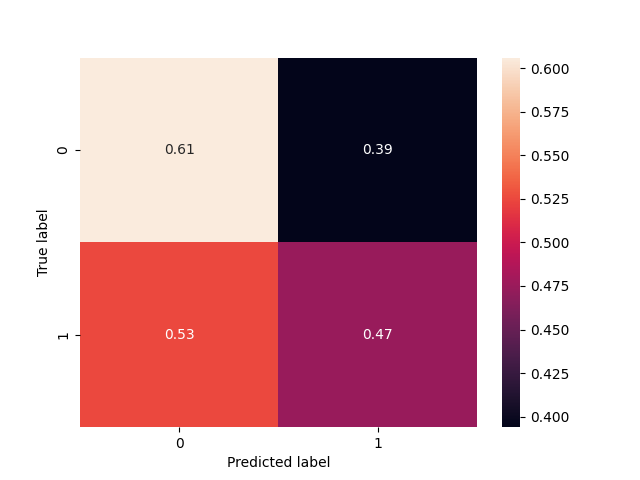
\includegraphics[width=\linewidth]{figures/results/word_embeddings/nn/calibrate/calibrate_set_6_confusion_matrix_percent.png}
%     \endminipage
%     \caption{Matrices de confusión en validación cruzada y el conjunto de test}
%     \end{subfigure}
%     \caption{Resultados del modelo de redes neuronales con codificación por word embeddings y esquema de acción calibrate.}
% \end{figure}

% \begin{table}[h!]
% \centering
% \scalebox{0.9}{
%  \begin{tabular}{|c || c | c | c | c | c | c |} 
%  \hline
%   Esquemas & Precisión & Recall & $H_{1.5}$ & $F_{1.5}$ & Umbral de decisión &
%   Modelo \\
%  \hline
%  take\_image & 0.8088 & 0.997 & 0.4351 & 0.997 & 0.61 & LGR \\
%  calibrate & 0.0467 & 0.4743 & 0.5083 & 0.1242 & 0.728 & NN\\
%  switch\_on  & 0.0405 & 0.4567 & 0.5106 & 0.1097 & 0.576 & NN\\
%  switch\_off & 0.0476 & 0.1818 & 0.2422 & 0.0876 & 0.034 & NN \\
%  turn\_to  & - & - & - & - & - & -\\[1ex]
%  \hline
%  \end{tabular}}
%  \caption{Resultados por esquema de acción del mejor modelo con codificación por word embeddings.}
%  \label{results:ad-hoc-calibrate}
% \end{table}


\section{Modelos predictivos ad-hoc}
\label{exp:wb}

\subsection{Configuración del experimento}

Para esta sección usaremos la codificación ad-hoc, bajo el mismo conjunto de
entrenamientos, construcción de ventanas, y configuraciones de búsqueda de los
modelos.

Describiremos el mejor modelo que obtuvimos con la codificación ad-hoc sobre un
esquema de acción distinto. En particular, el esquema \emph{calibrate} y el
perceptrón multicapa como modelo de aprendizaje.

\subsection{Resultados}

\subsubsection{Performance en validación cruzada}

La figura \ref{fig:calibrate-bestmodel-adhoc} muestra la distribución de las
predicciones en validación cruzada para la mejor configuración de parámetros de
NN. Si observamos los histogramas de la clase positiva, tenemos que aproximadamente
el 90\% de las acciones etiquetadas como positivas se agrupan en el intervalo $r
= [0.8; 1]$ mientras que de las negativas solo un 10\% al 20\% se encuentra en
$r$. Además, la mayoria de acciones negativas tienen probabilidades en el rango
del $[0;0.4]$ lo cual nuevamente estamos ante un muy buen desempeño en
validación cruzada en terminos de grounding heurístico.

\begin{figure}[b!]
    \centering
    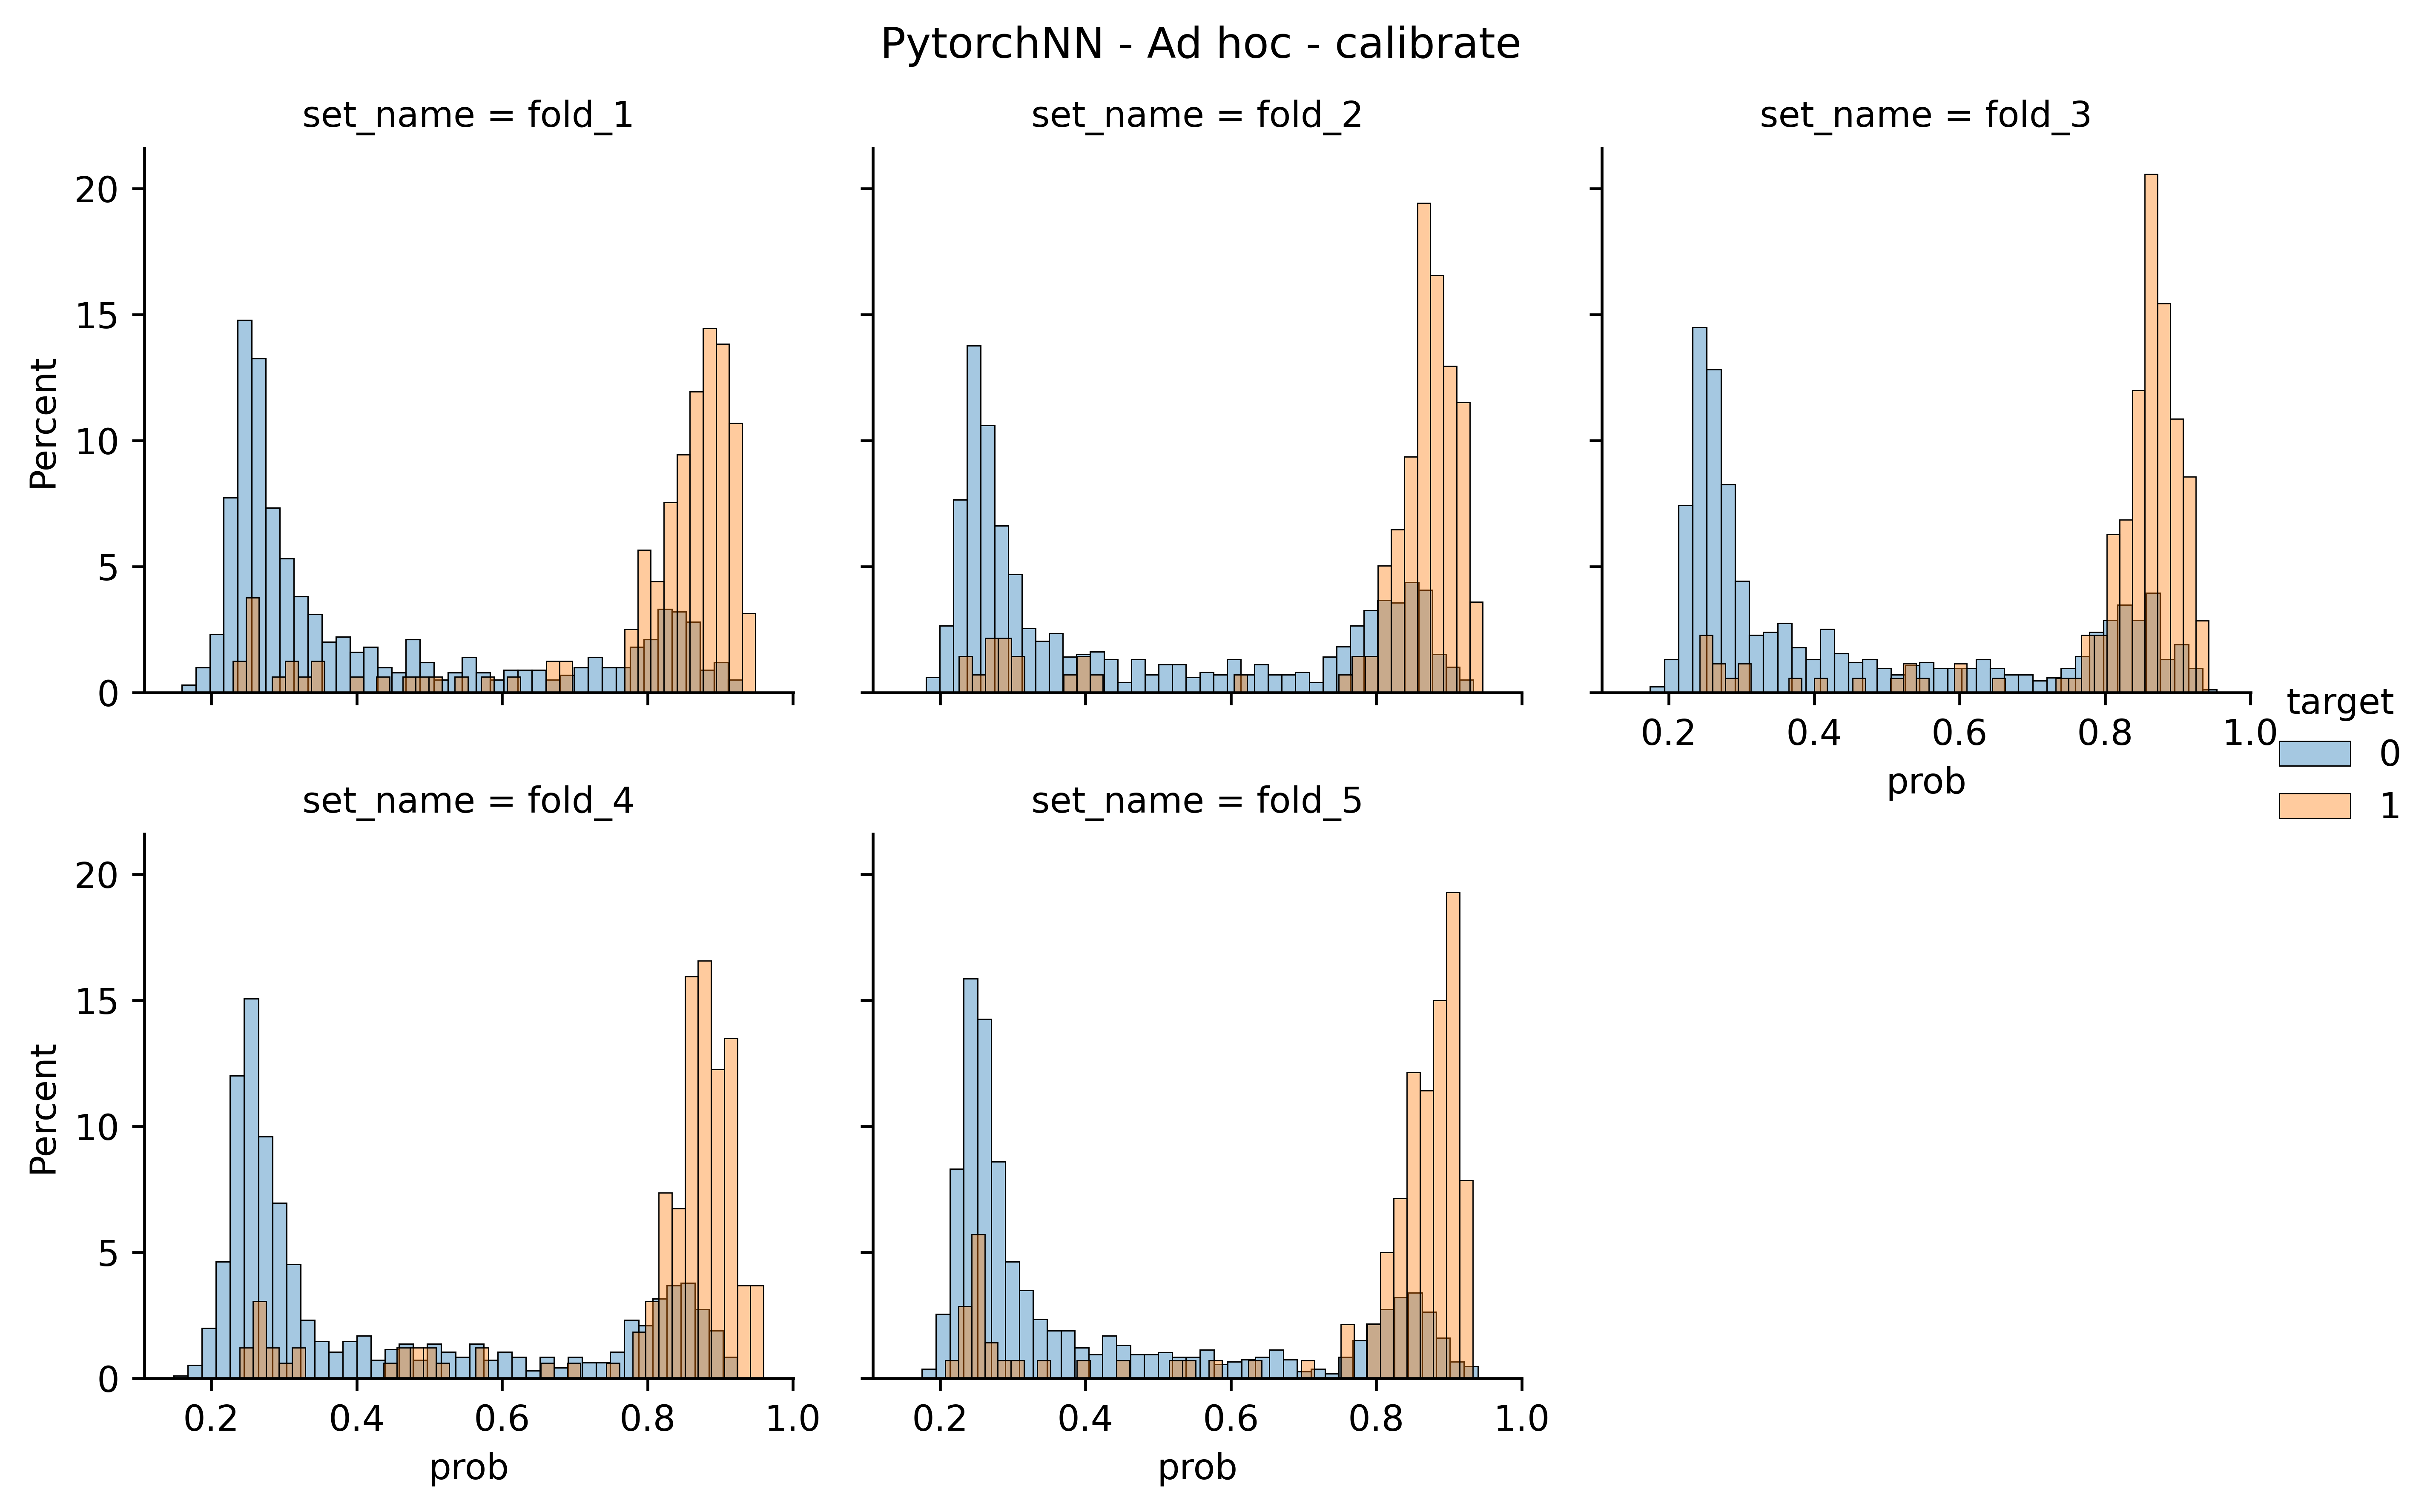
\includegraphics[width=\linewidth]{figures/results/ad-hoc/nn/calibrate/nn_adhoc_calibrate.png}
    \caption{Distribución de predicciones en validación cruzada sobre el modelo NN ad-hoc.}
    \label{fig:calibrate-bestmodel-adhoc}
\end{figure}

\begin{table}[h!]
    \centering
    \scalebox{1}{
     \begin{tabular}{|c || c | c | c | c | c | c |} 
     \hline
      Clase & Fold & Precisión & Recall & $H_{1.5}$ & $F_{1.5}$ & Umbral de decisión \\
     \hline
     Relevante &  1 & 0.31 & 0.85 & - & - & 0.7\\
     No relevante & 1 & 0.97 & 0.71 & - & - & 0.7 \\
     \hline
     Relevante & 2 & 0.26 & 0.87 & - & - & 0.77 \\
     No relevante & 2 & 0.98 & 0.68 & - & - & 0.77 \\
     \hline
     Relevante & 3 & 0.3 & 0.9 & - & - & 0.72 \\
     No relevante & 3 & 0.97 & 0.0.63 & - & - & 0.72\\
     \hline
     Relevante & 4 & 0.31 & 0.86 & - & - & 0.75\\
     No relevante & 4 & 0.97 & 0.0.7 & - & - & 0.75\\
     \hline
     Relevante & 5 & 0.26 & 0.87 & -  & - & 0.57 \\
     No relevante & 5 & 0.98 & 0.7 & - & - & 0.57 \\
     \hline
     \end{tabular}}
     \caption{Métricas sobre el conjunto de test del modelo NN ad-hoc.}
     \label{results:nn-adhoc-calibrate}
\end{table}

El cuadro \ref{results:nn-adhoc-calibrate} muestra los resultados de predicción
por cada fold. Notar como el umbral de decisión optimizado por $H_{1.5}$ llegó a
alcanzar hasta un valor de 0.77 en el segundo fold. Aún para este valor de
umbral, los resultados en \emph{precision} no fueron muy altos para la clase
positiva. Recordemos que \emph{precision} en clase positiva penaliza los
falsos positivos (FPs). Observando el gráfico de distribuciones, el umbral
estaría separando adecuadamente las clases relevantes de las irrelevantes por lo
cual no se logra observar el porque de estos resultados en \emph{precision} con
este gráfico.

Sin embargo, si en lugar de considerar las distribuciones revisamos las matrices
de confusión sin normalizar (Figura \ref{fig:calibrate-bestmodel-cm}),
observamos que los datos se encuentran desbalanceados para la clase 0.
Asemejandose a lo que usualmente ocurre con los problemas de planning donde los
good operators suelen ser menor en cantidad a los bad operators. En particular,
esto puede ser un problema para \emph{precision} dado que penaliza por la
cantidad de FPs. Por ejemplo, si observamos el primer fold de la validación
cruzada, se logra predecir correctamente por encima del 70\% de las acciones no
relevantes. Sin embargo, esto es relativo a la cantidad de acciones que tengamos
de la clase 0. Si tenemos en cuenta la formula de \emph{precision}:

\begin{align*}
    precision = TP / (TP + FP)
\end{align*}

Se logra observar que al depender de los FPs, entonces también depende de la
cantidad de desbalance que tenga el conjunto de datos. De hecho, si se
incrementa la cantidad de bad operators, pero las proporciones 70-30\% se
mantienen, la métrica disminuiria. Sin embargo, en términos de grounding
heurístico el modelo seguiría desempeñandose correctamente.

\begin{figure}[t!]
    \minipage{0.50\textwidth}
    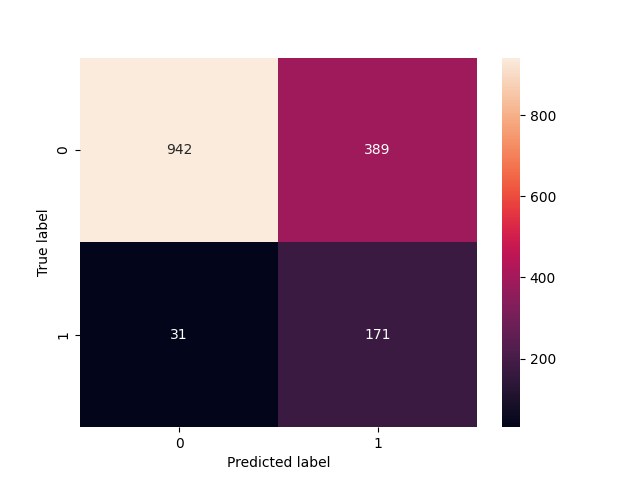
\includegraphics[width=\linewidth]{figures/results/ad-hoc/nn/calibrate/2021-12-06_17.03.17.314982_set_1_confusion_matrix_raw.png}
    \endminipage
    \minipage{0.50\textwidth}
    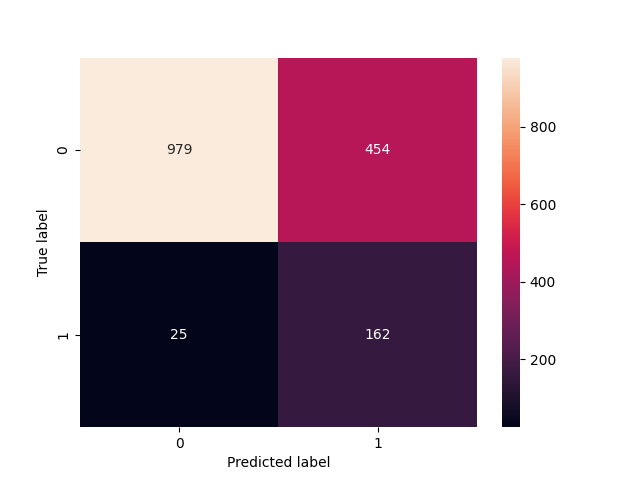
\includegraphics[width=\linewidth]{figures/results/ad-hoc/nn/calibrate/2021-12-06_17.03.17.314982_set_2_confusion_matrix_raw.png}
    \endminipage
        
    \minipage{0.50\textwidth}%
    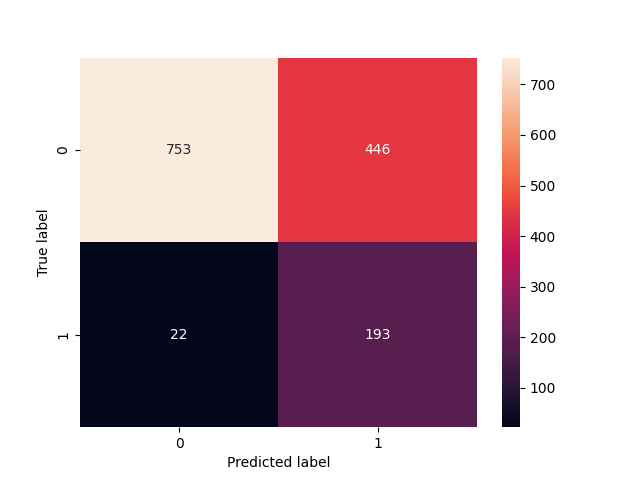
\includegraphics[width=\linewidth]{figures/results/ad-hoc/nn/calibrate/2021-12-06_17.03.17.314982_set_3_confusion_matrix_raw.png}
    \endminipage
    \minipage{0.50\textwidth}
    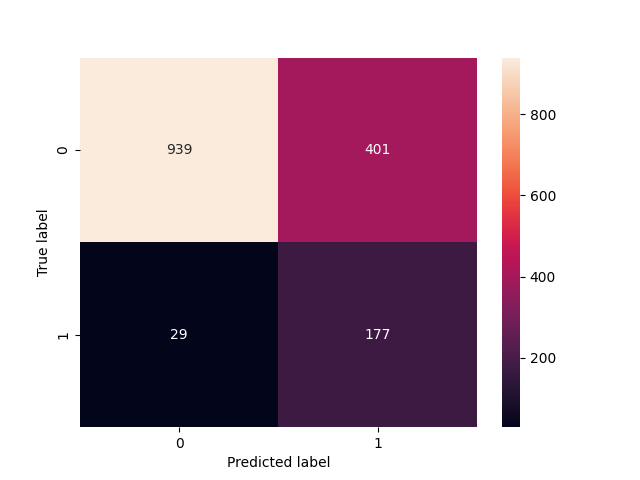
\includegraphics[width=\linewidth]{figures/results/ad-hoc/nn/calibrate/2021-12-06_17.03.17.314982_set_4_confusion_matrix_raw.png}
    \endminipage

    \minipage{0.50\textwidth}
    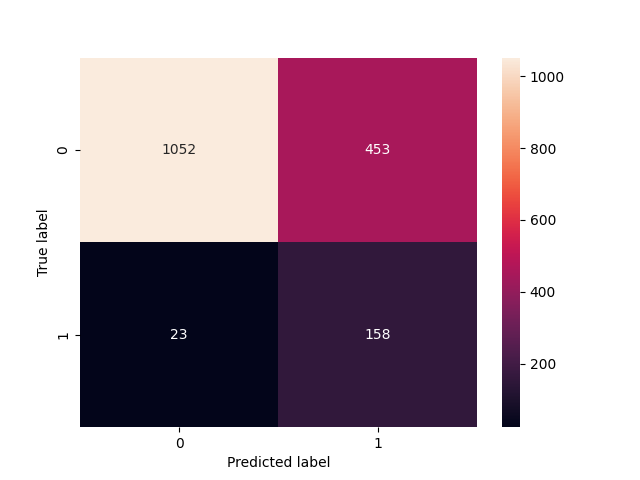
\includegraphics[width=\linewidth]{figures/results/ad-hoc/nn/calibrate/2021-12-06_17.03.17.314982_set_5_confusion_matrix_raw.png}
    \endminipage
    \caption{Matrices de confusión en validación cruzada para el modelo NN ad-hoc.}
    \label{fig:calibrate-bestmodel-cm}
\end{figure}

\subsubsection{Performance en test}

\begin{figure}[b!]
    \begin{subfigure}[b]{\textwidth}
        \centering
        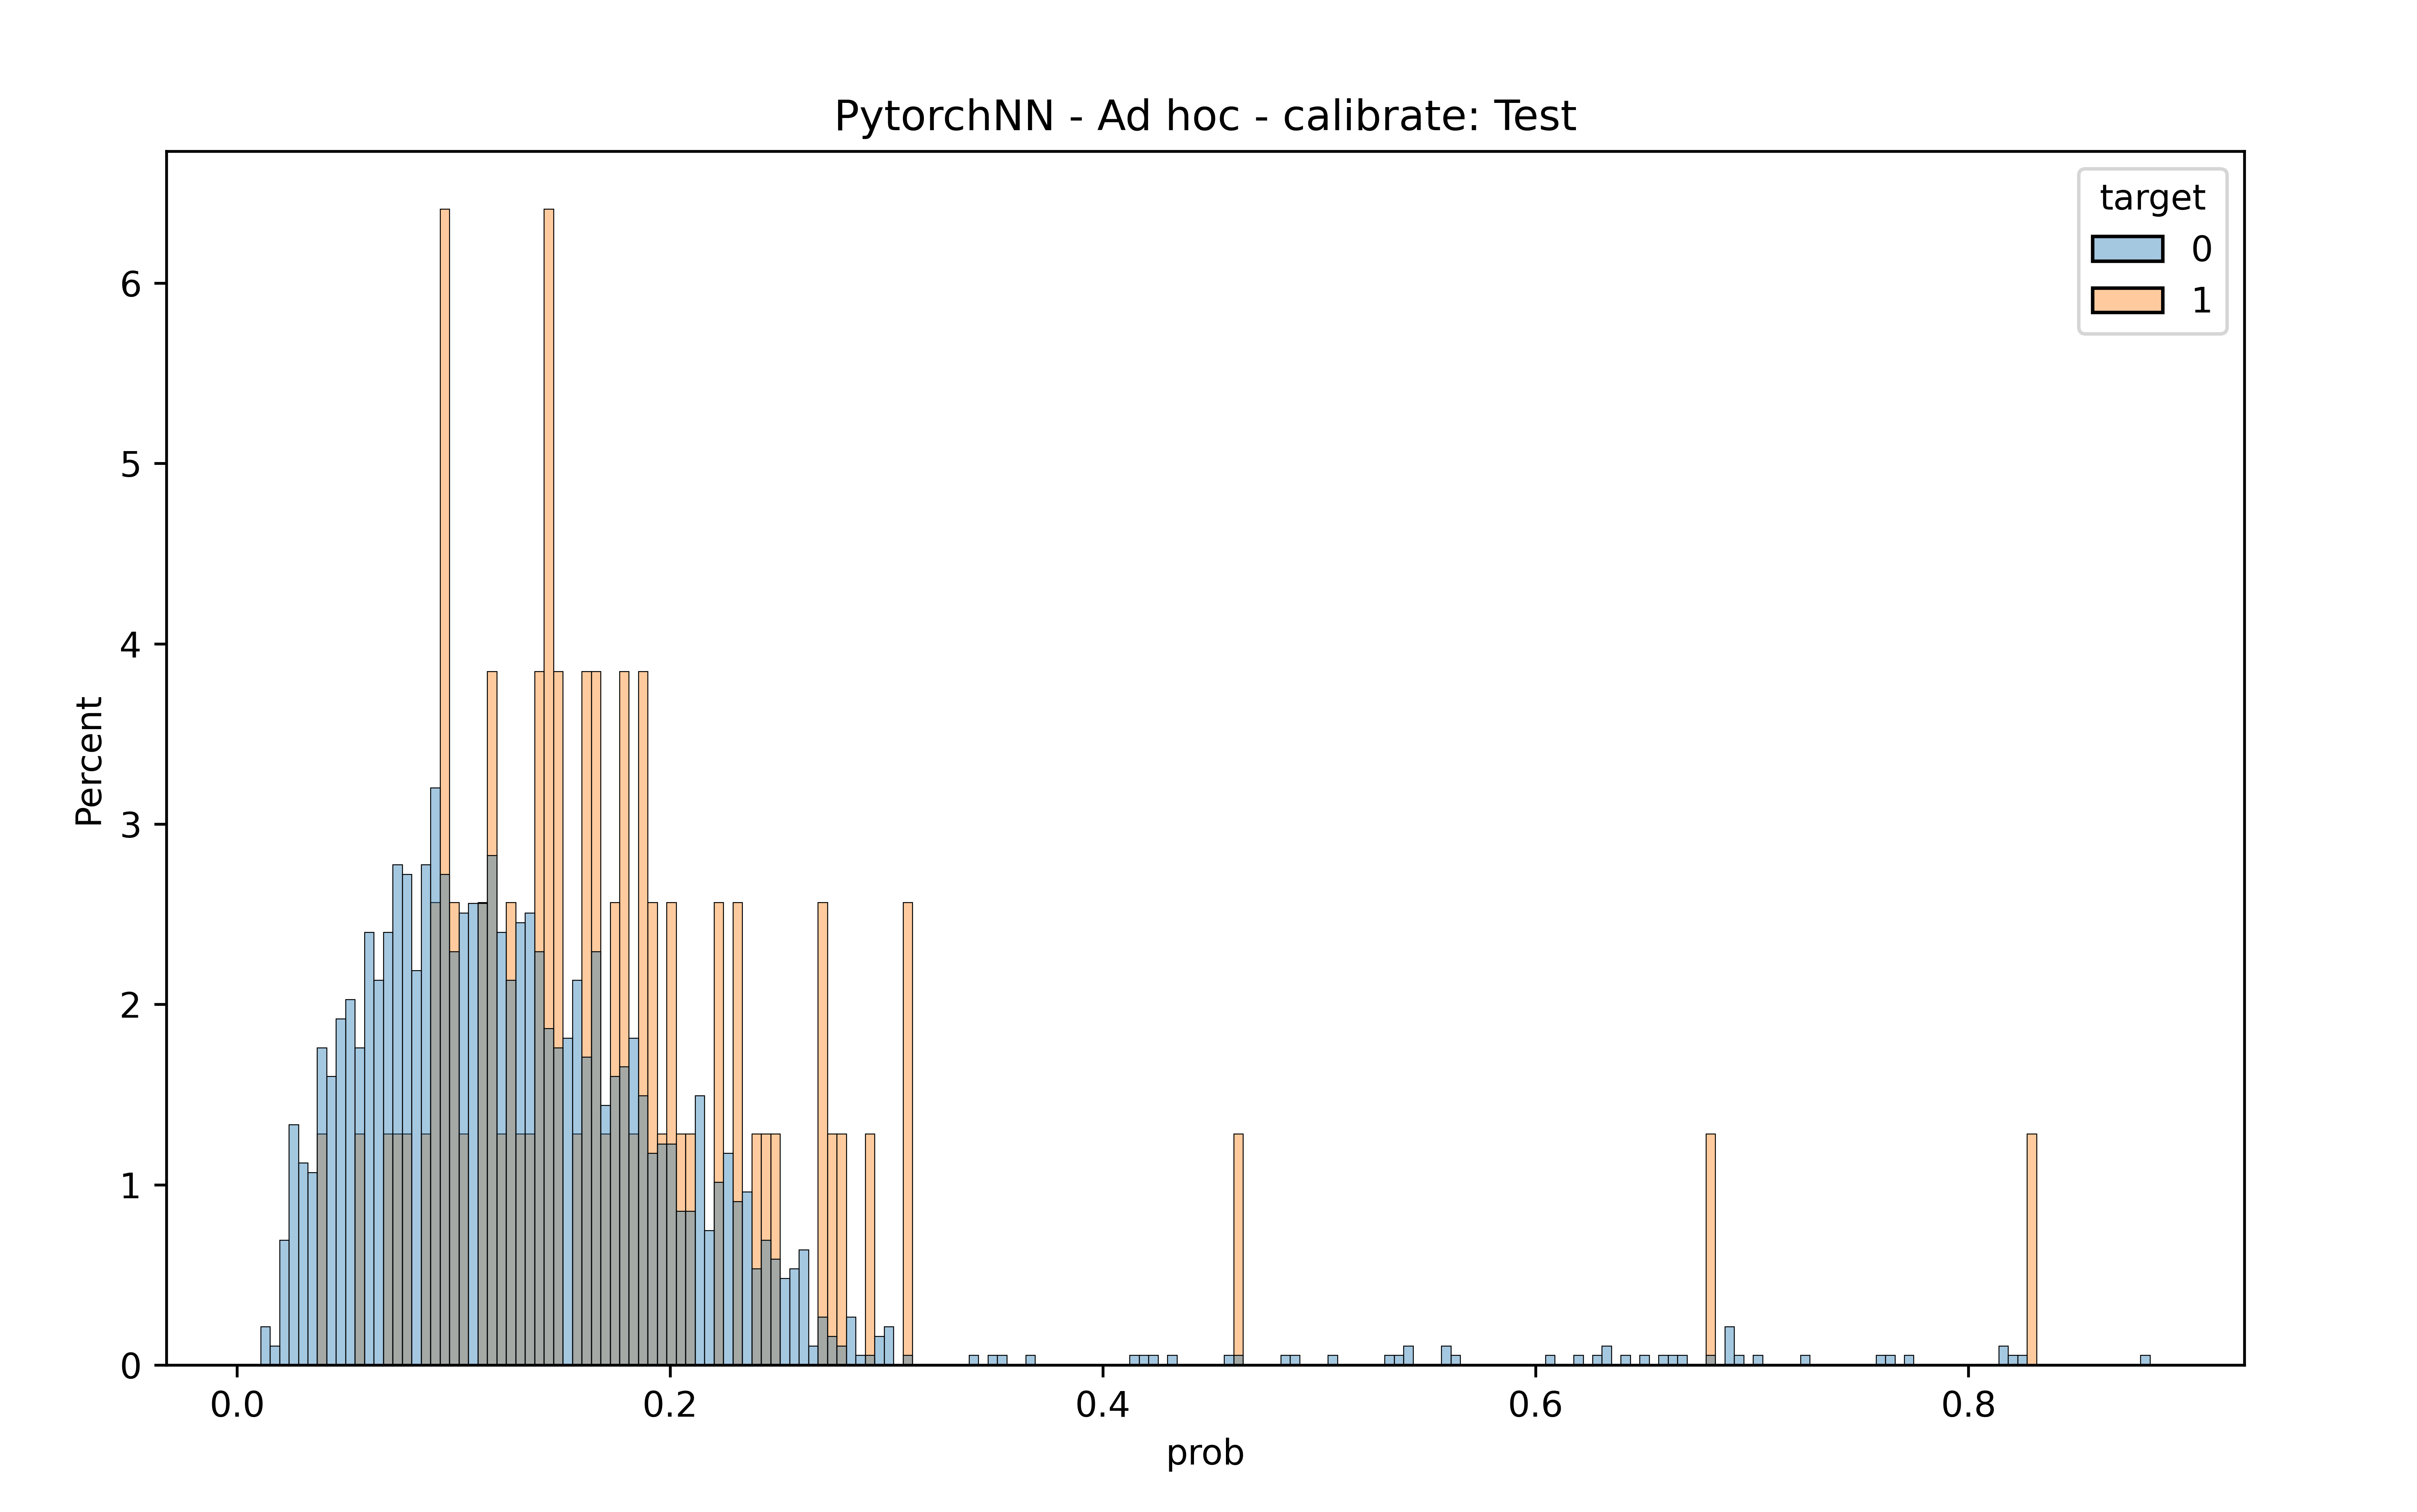
\includegraphics[width=0.7\linewidth]{figures/results/ad-hoc/nn/calibrate/nn_adhoc_calibrate_test.png}
        \caption{Distribución de predicciones}
        \label{fig:calibrate-bestmoodel-adhoc-test}
    \end{subfigure}
    \begin{subfigure}[b]{\textwidth}
        \centering
        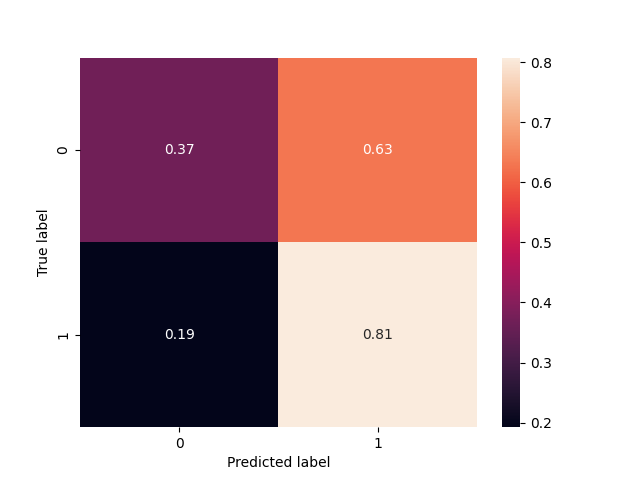
\includegraphics[width=0.7\linewidth]{figures/results/ad-hoc/nn/calibrate/NN_cm_test.png}
        \caption{Matriz de confusión}
        \label{fig:calibrate-bestmoodel-adhoc-test}
    \end{subfigure}
    \caption{Resultados en el conjunto de test para el modelo NN ad-hoc.}
\end{figure}

Nuevamente, lo que buscamos es que este modelo logre generalizar a problemas no
instanciables. La figura \ref{fig:calibrate-bestmoodel-adhoc-test} muestra como
se distribuyen las probabilidades que el modelo asigna a las acciones participes
del conjunto de test. Se puede observar un comportamiento muy distinto al que
ocurrió en validación cruzada. El umbral de predicción promedio obtenido en
validación cruzada es de 0.702. Bajo ese umbral, el modelo predice que todas las
acciones son irrelevantes obteniendo una performance practicamente nula. Por lo
que a primera impresión parecería que no es un modelo que podamos utilizar en
grounding heurístico. De hecho, un resultado como este para un problema clásico
de aprendizaje automático llevaría a descartar la solución y probar con otra
configuración. No obstante, en el contexto de grounding heúrstico, buscamos que
las acciones relevantes para encontrar un plan tengan una probabilidad superior
a las que no lo son. Sin importar en que parte del intervalo $[0;1]$ se asignen
las probabilidades. Mientras se respete el orden que necesitamos para ubicar las
acciones en la cola de prioridades, entonces podemos considerarlo como un buen
modelo. Es por eso la razón por la que el umbral de decisión tampoco se mantiene
fijo, y varia de acuerdo a $H_{beta}$. Para este problema el umbral es una
manera de cuantificar esta idea más cualitativa que buscamos en grounding
heurístico pero que es determinante en la elección del modelo de aprendizaje.

Por ejemplo, para un umbral de 0.1, podemos ver que el modelo se comporta de
manera similar al de \emph{take\_image}.

% \begin{figure}
%     \centering
%     \begin{subfigure}[b]{0.83\textwidth}
%     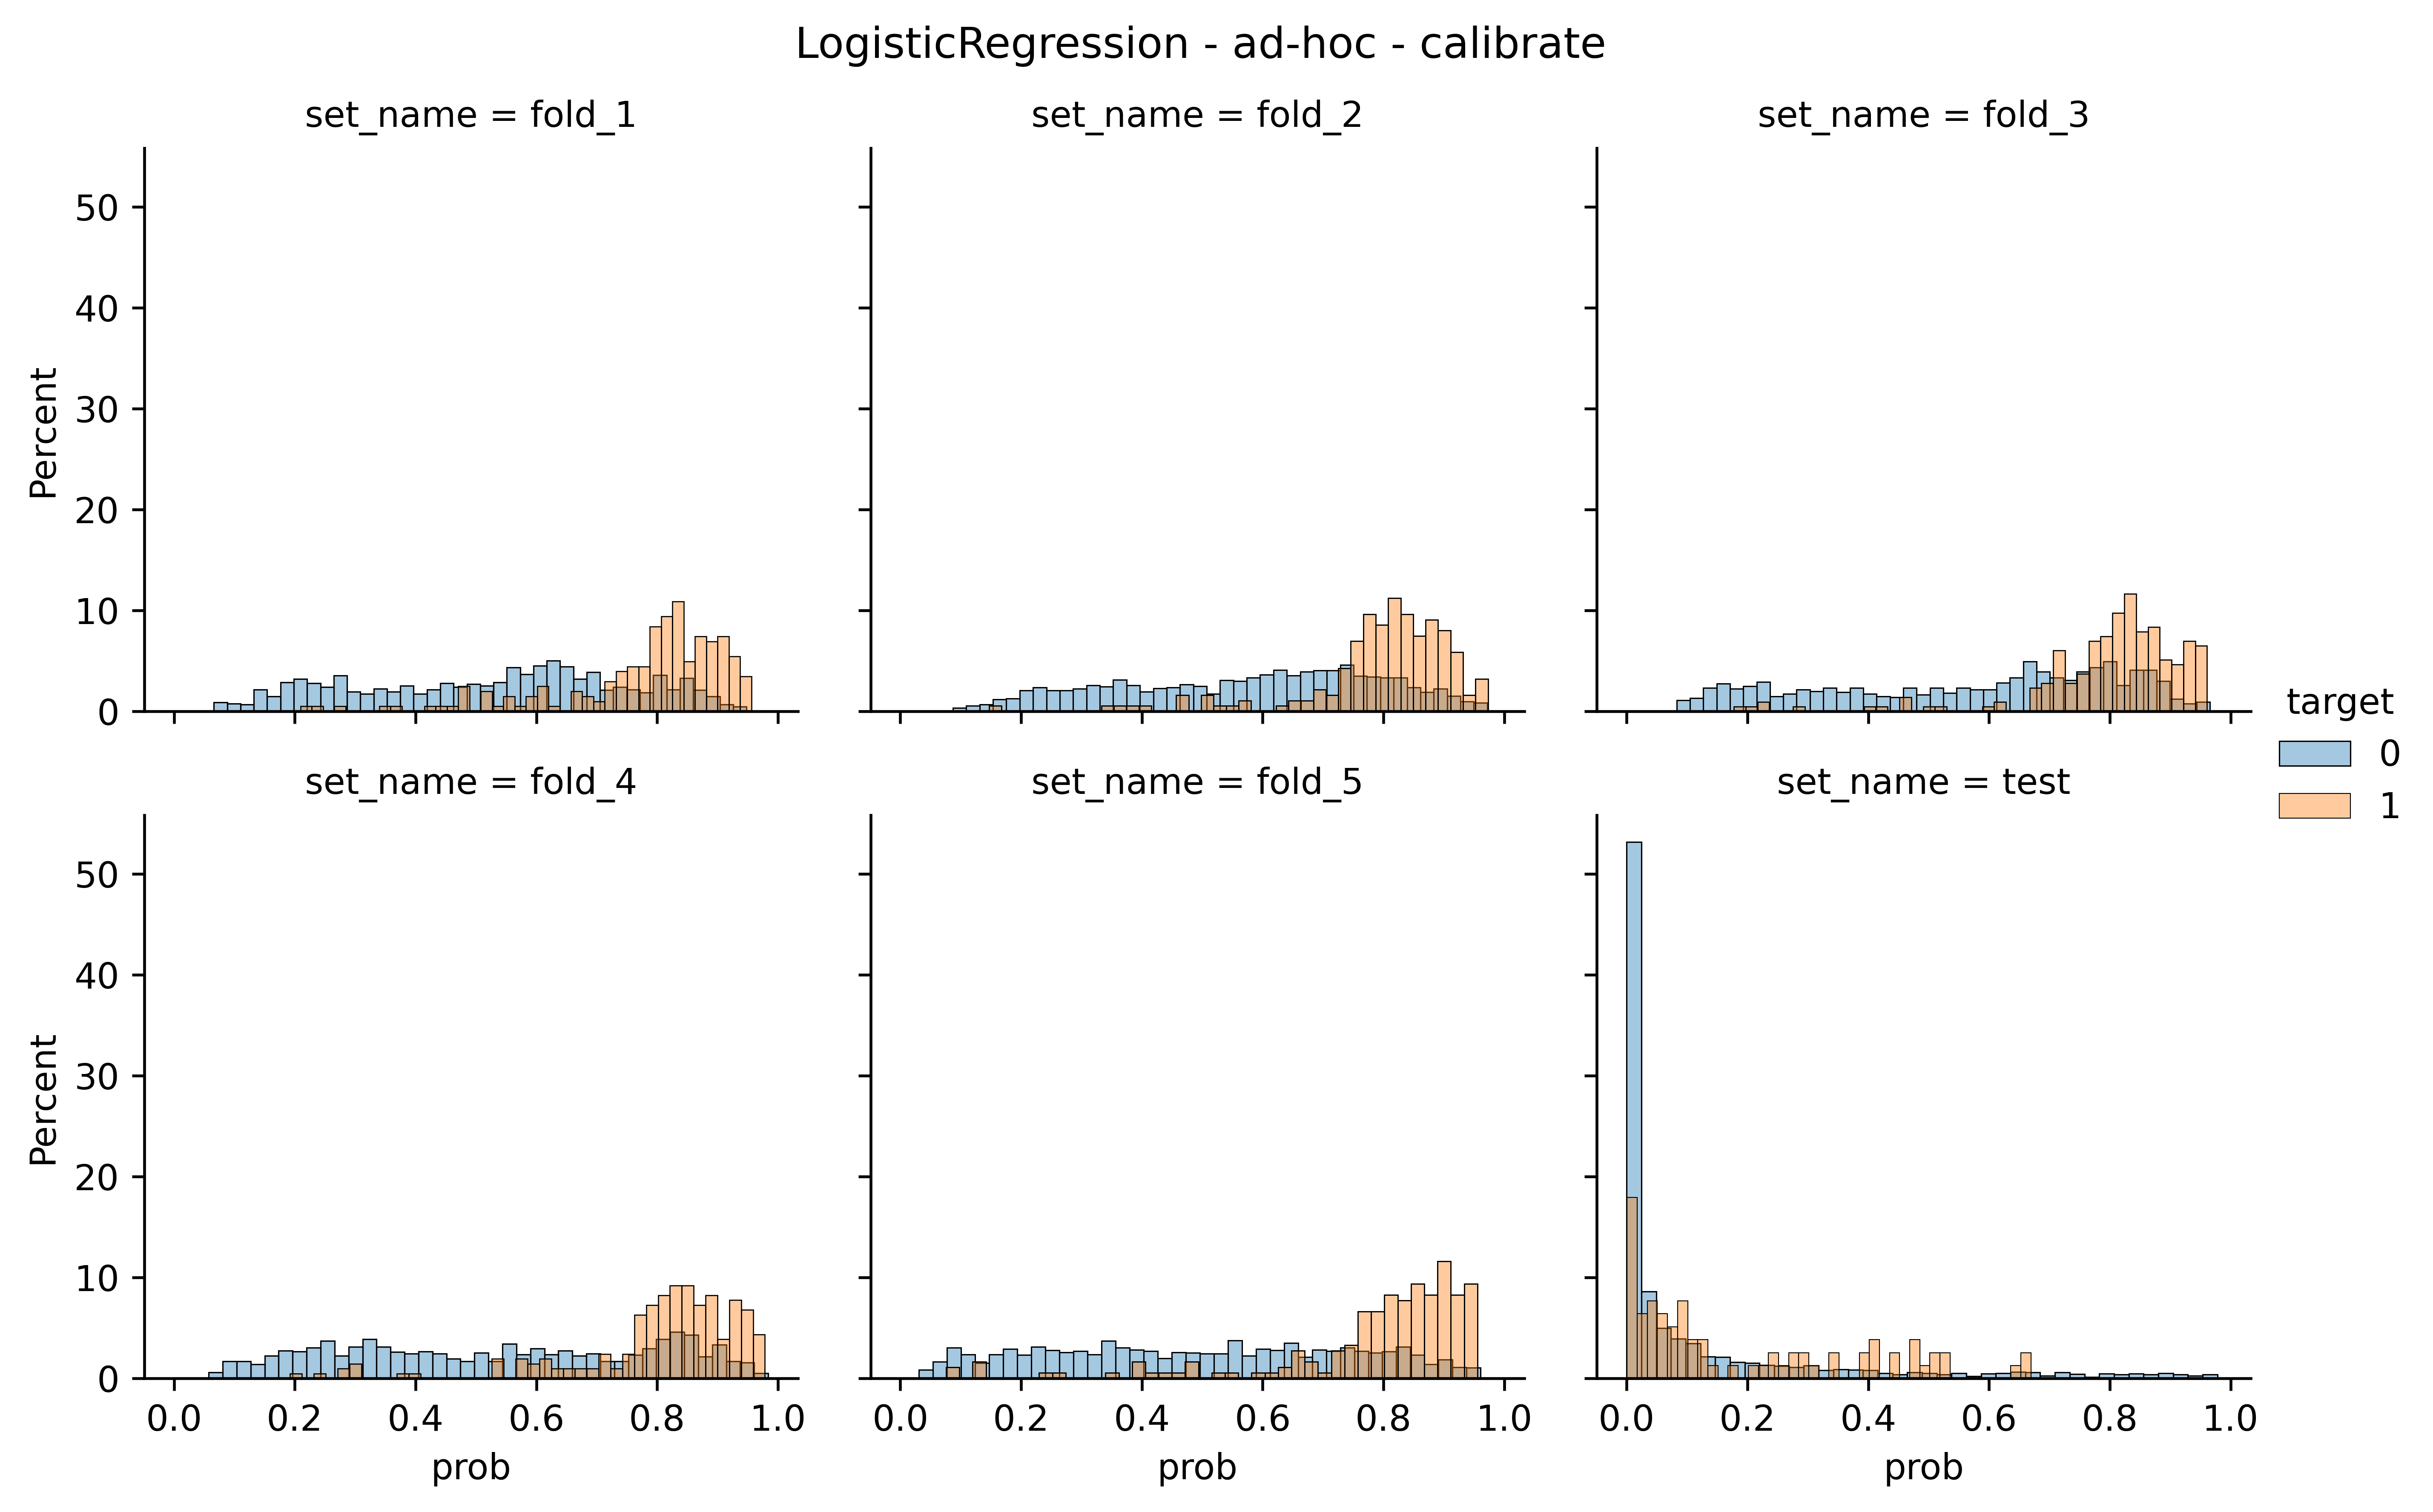
\includegraphics[width=\linewidth]{figures/results/ad-hoc/lgr/calibrate/calibrate__distplot.png}
%     \end{subfigure}
%     \hfill
%     \centering
%     \begin{subfigure}[b]{0.83\textwidth}
%         \centering
%         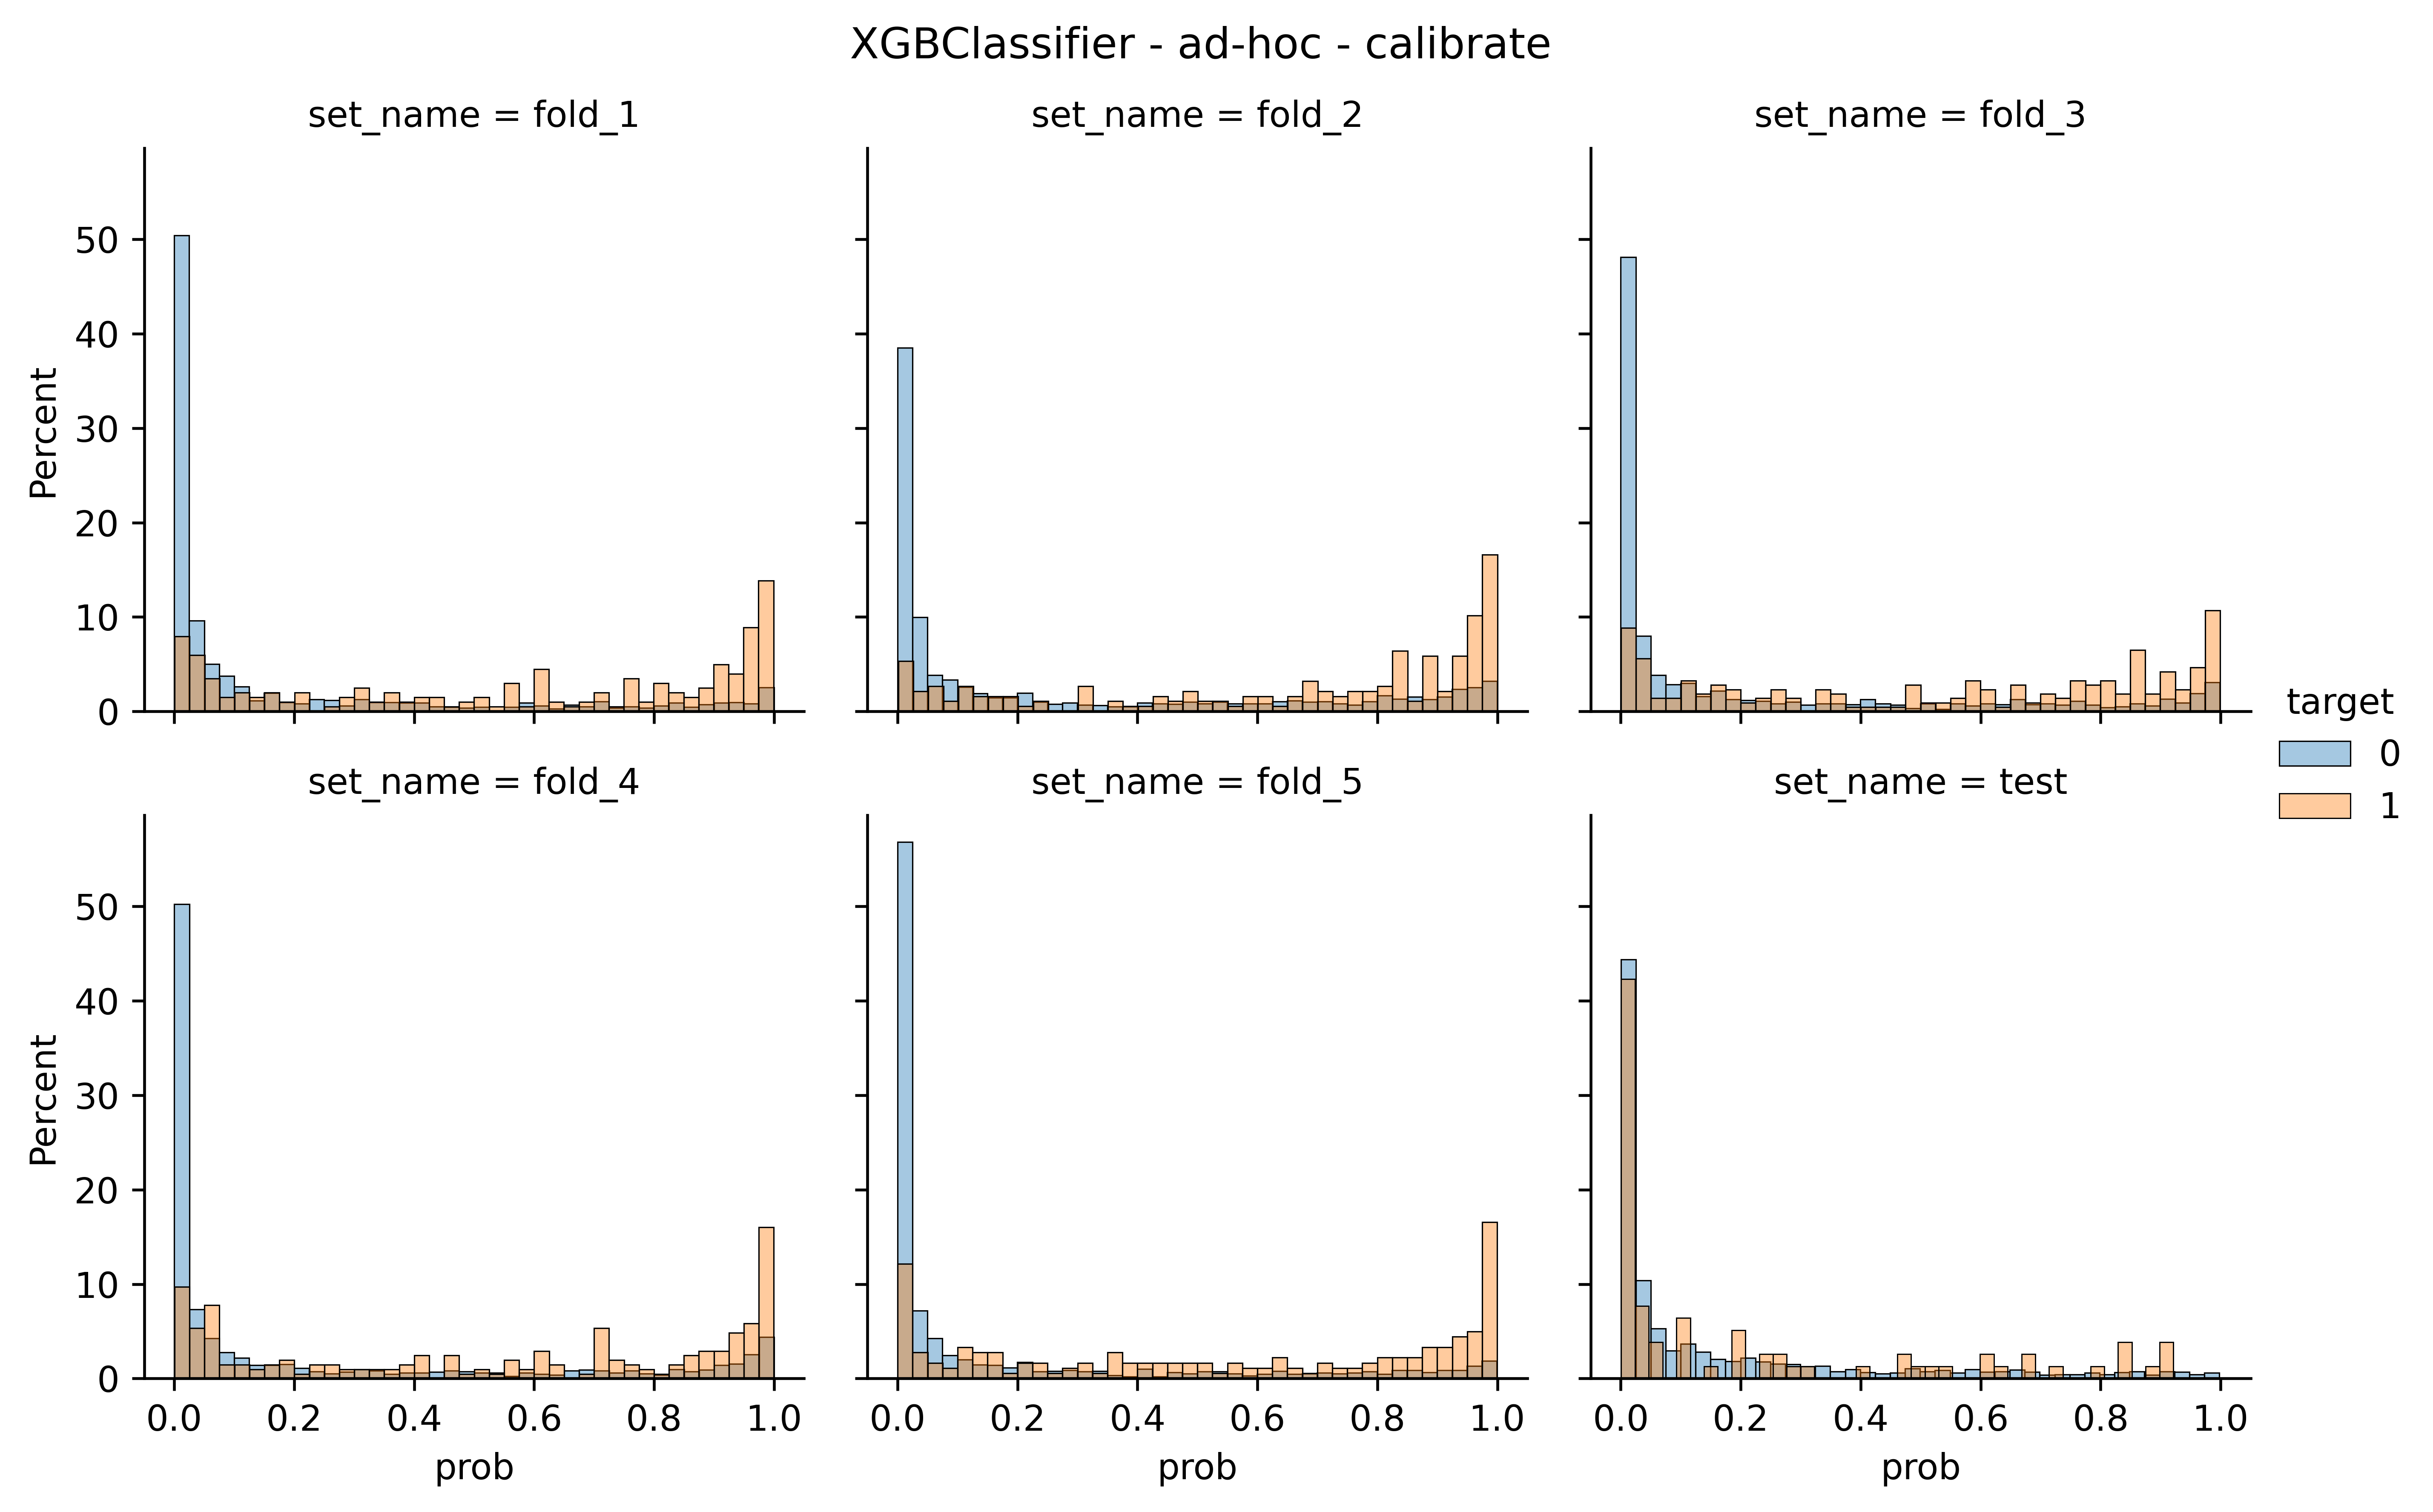
\includegraphics[width=\linewidth]{figures/results/ad-hoc/xgb/2021-12-07_06.29.19.600877__distplot (2).png}
%     \end{subfigure}
%     \hfill
%     \centering
%     \begin{subfigure}[b]{0.83\textwidth}
%         \centering
%         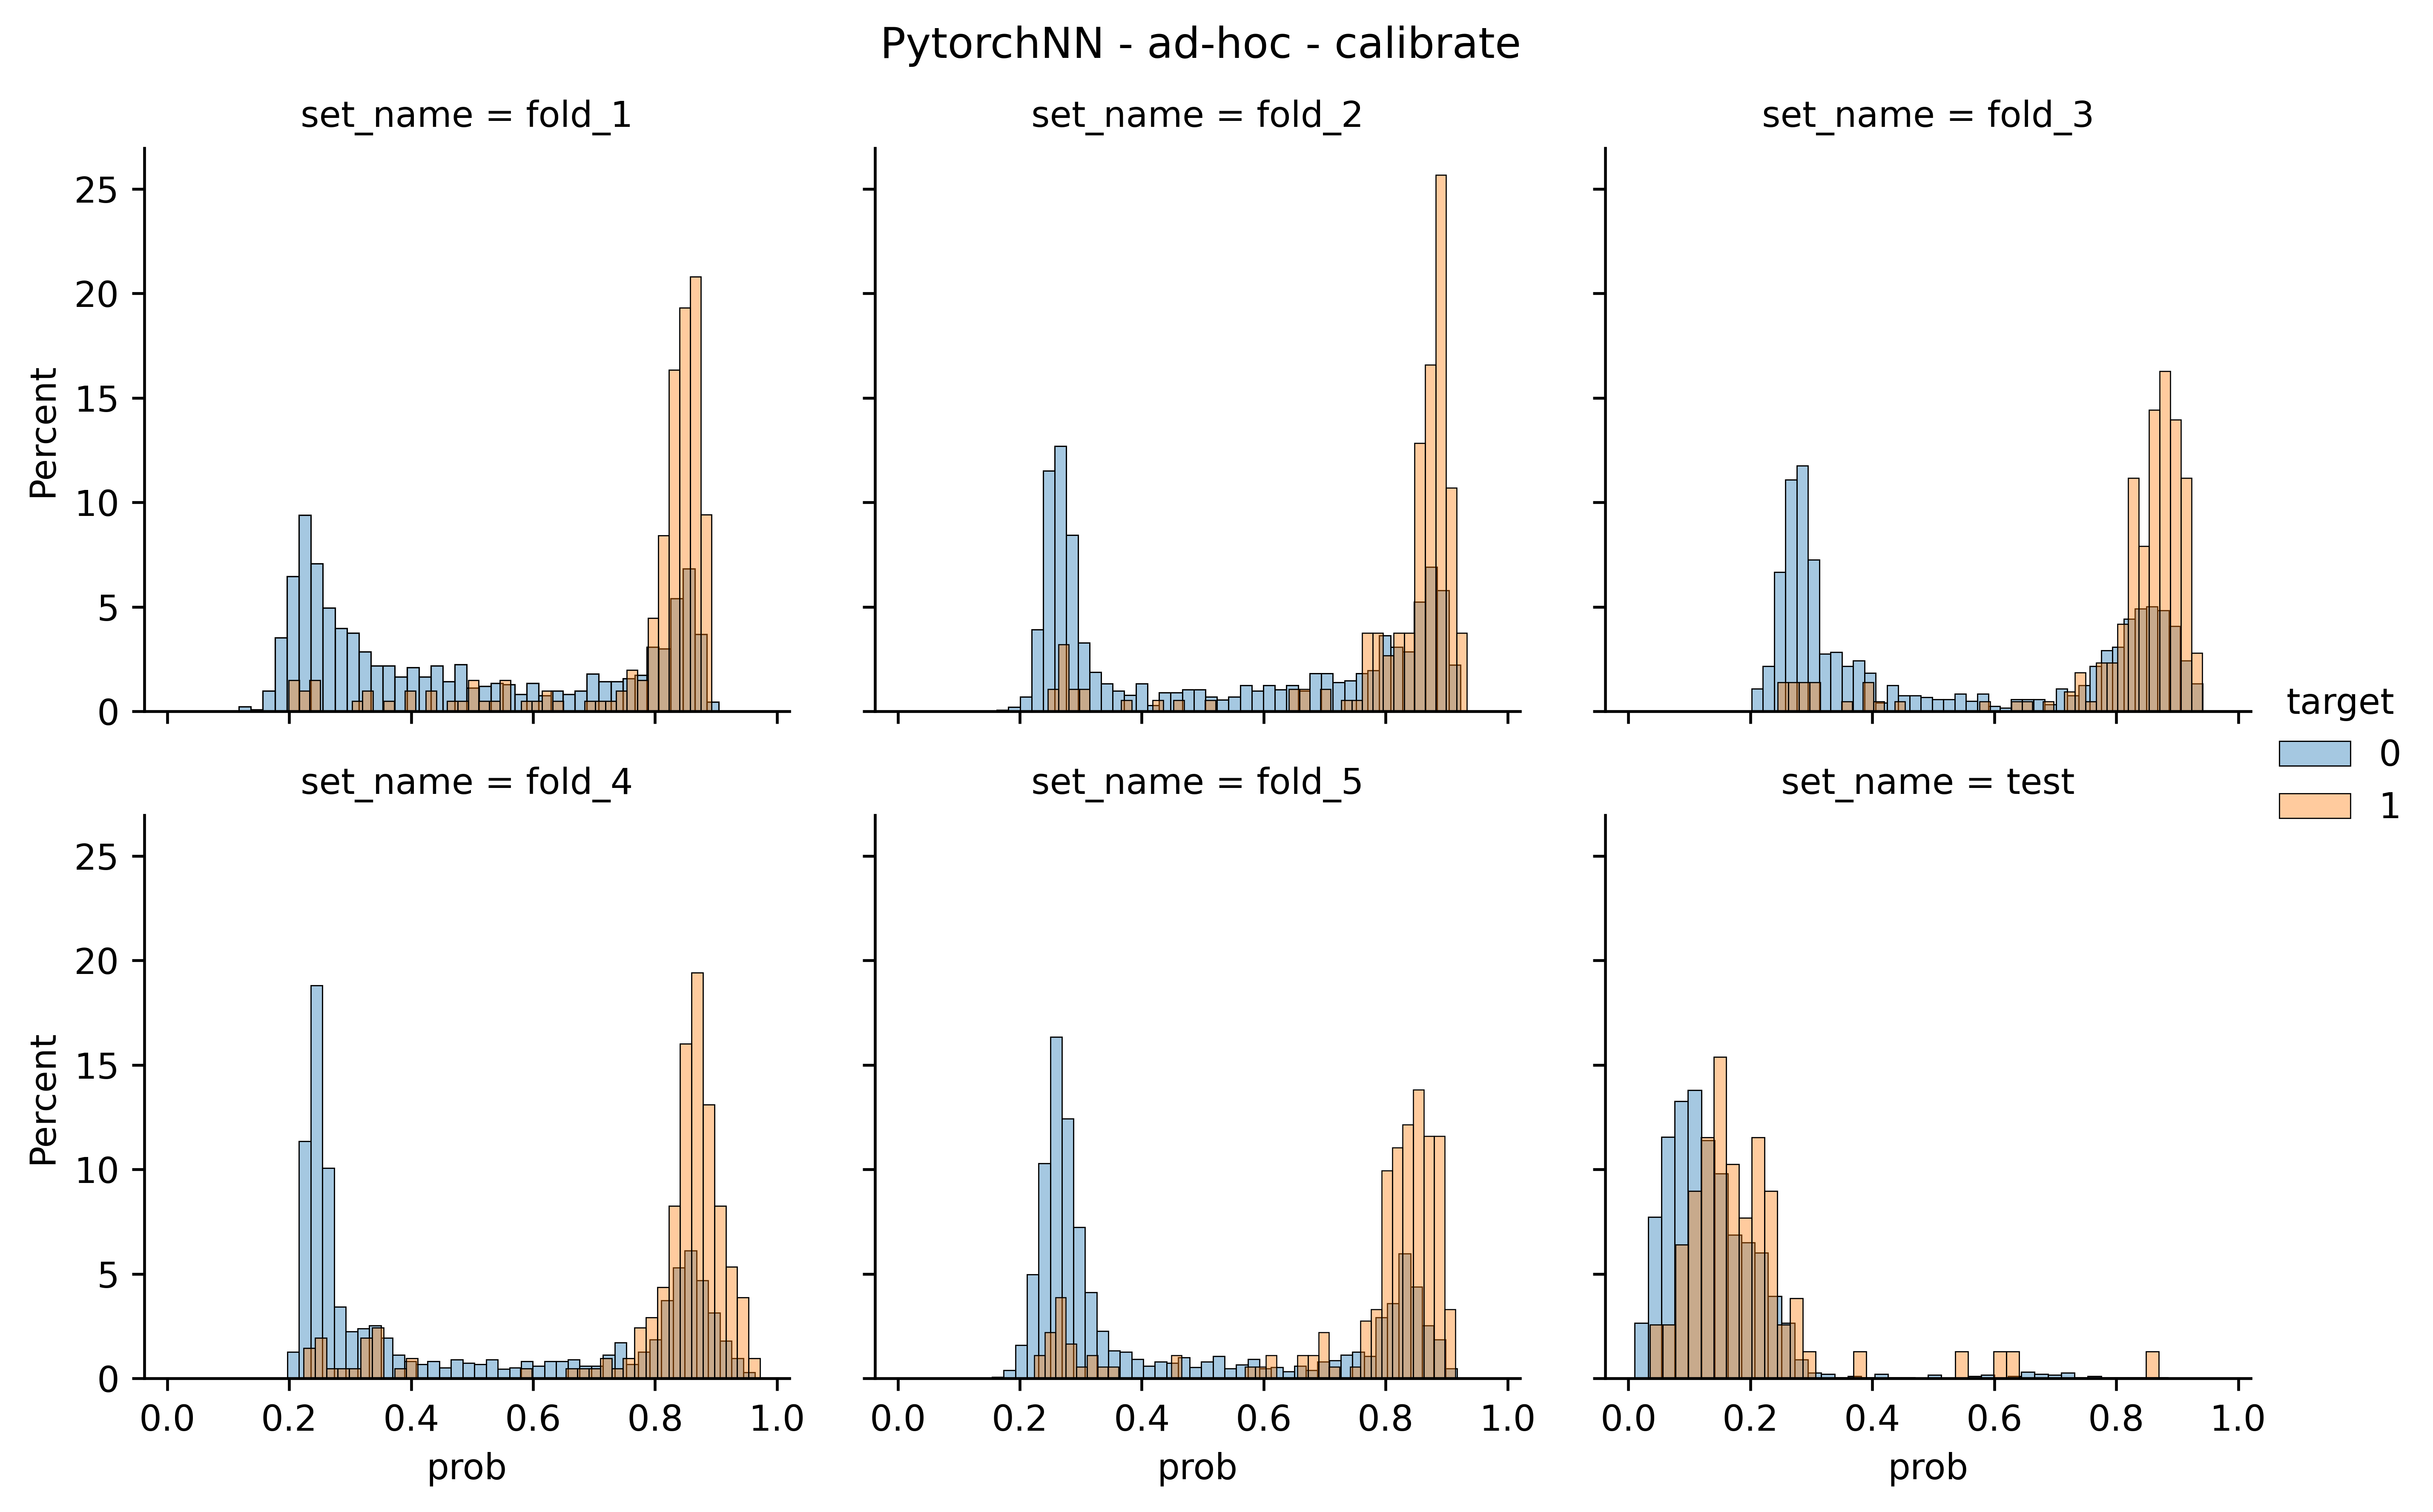
\includegraphics[width=\linewidth]{figures/results/ad-hoc/nn/2021-12-06_17.03.17.314982__distplot.png}
%     \end{subfigure}
%     \caption{Ad-hoc calibrate}
% \end{figure}
% 
% \begin{figure}
%     \centering
%     \begin{subfigure}[b]{0.83\textwidth}
%     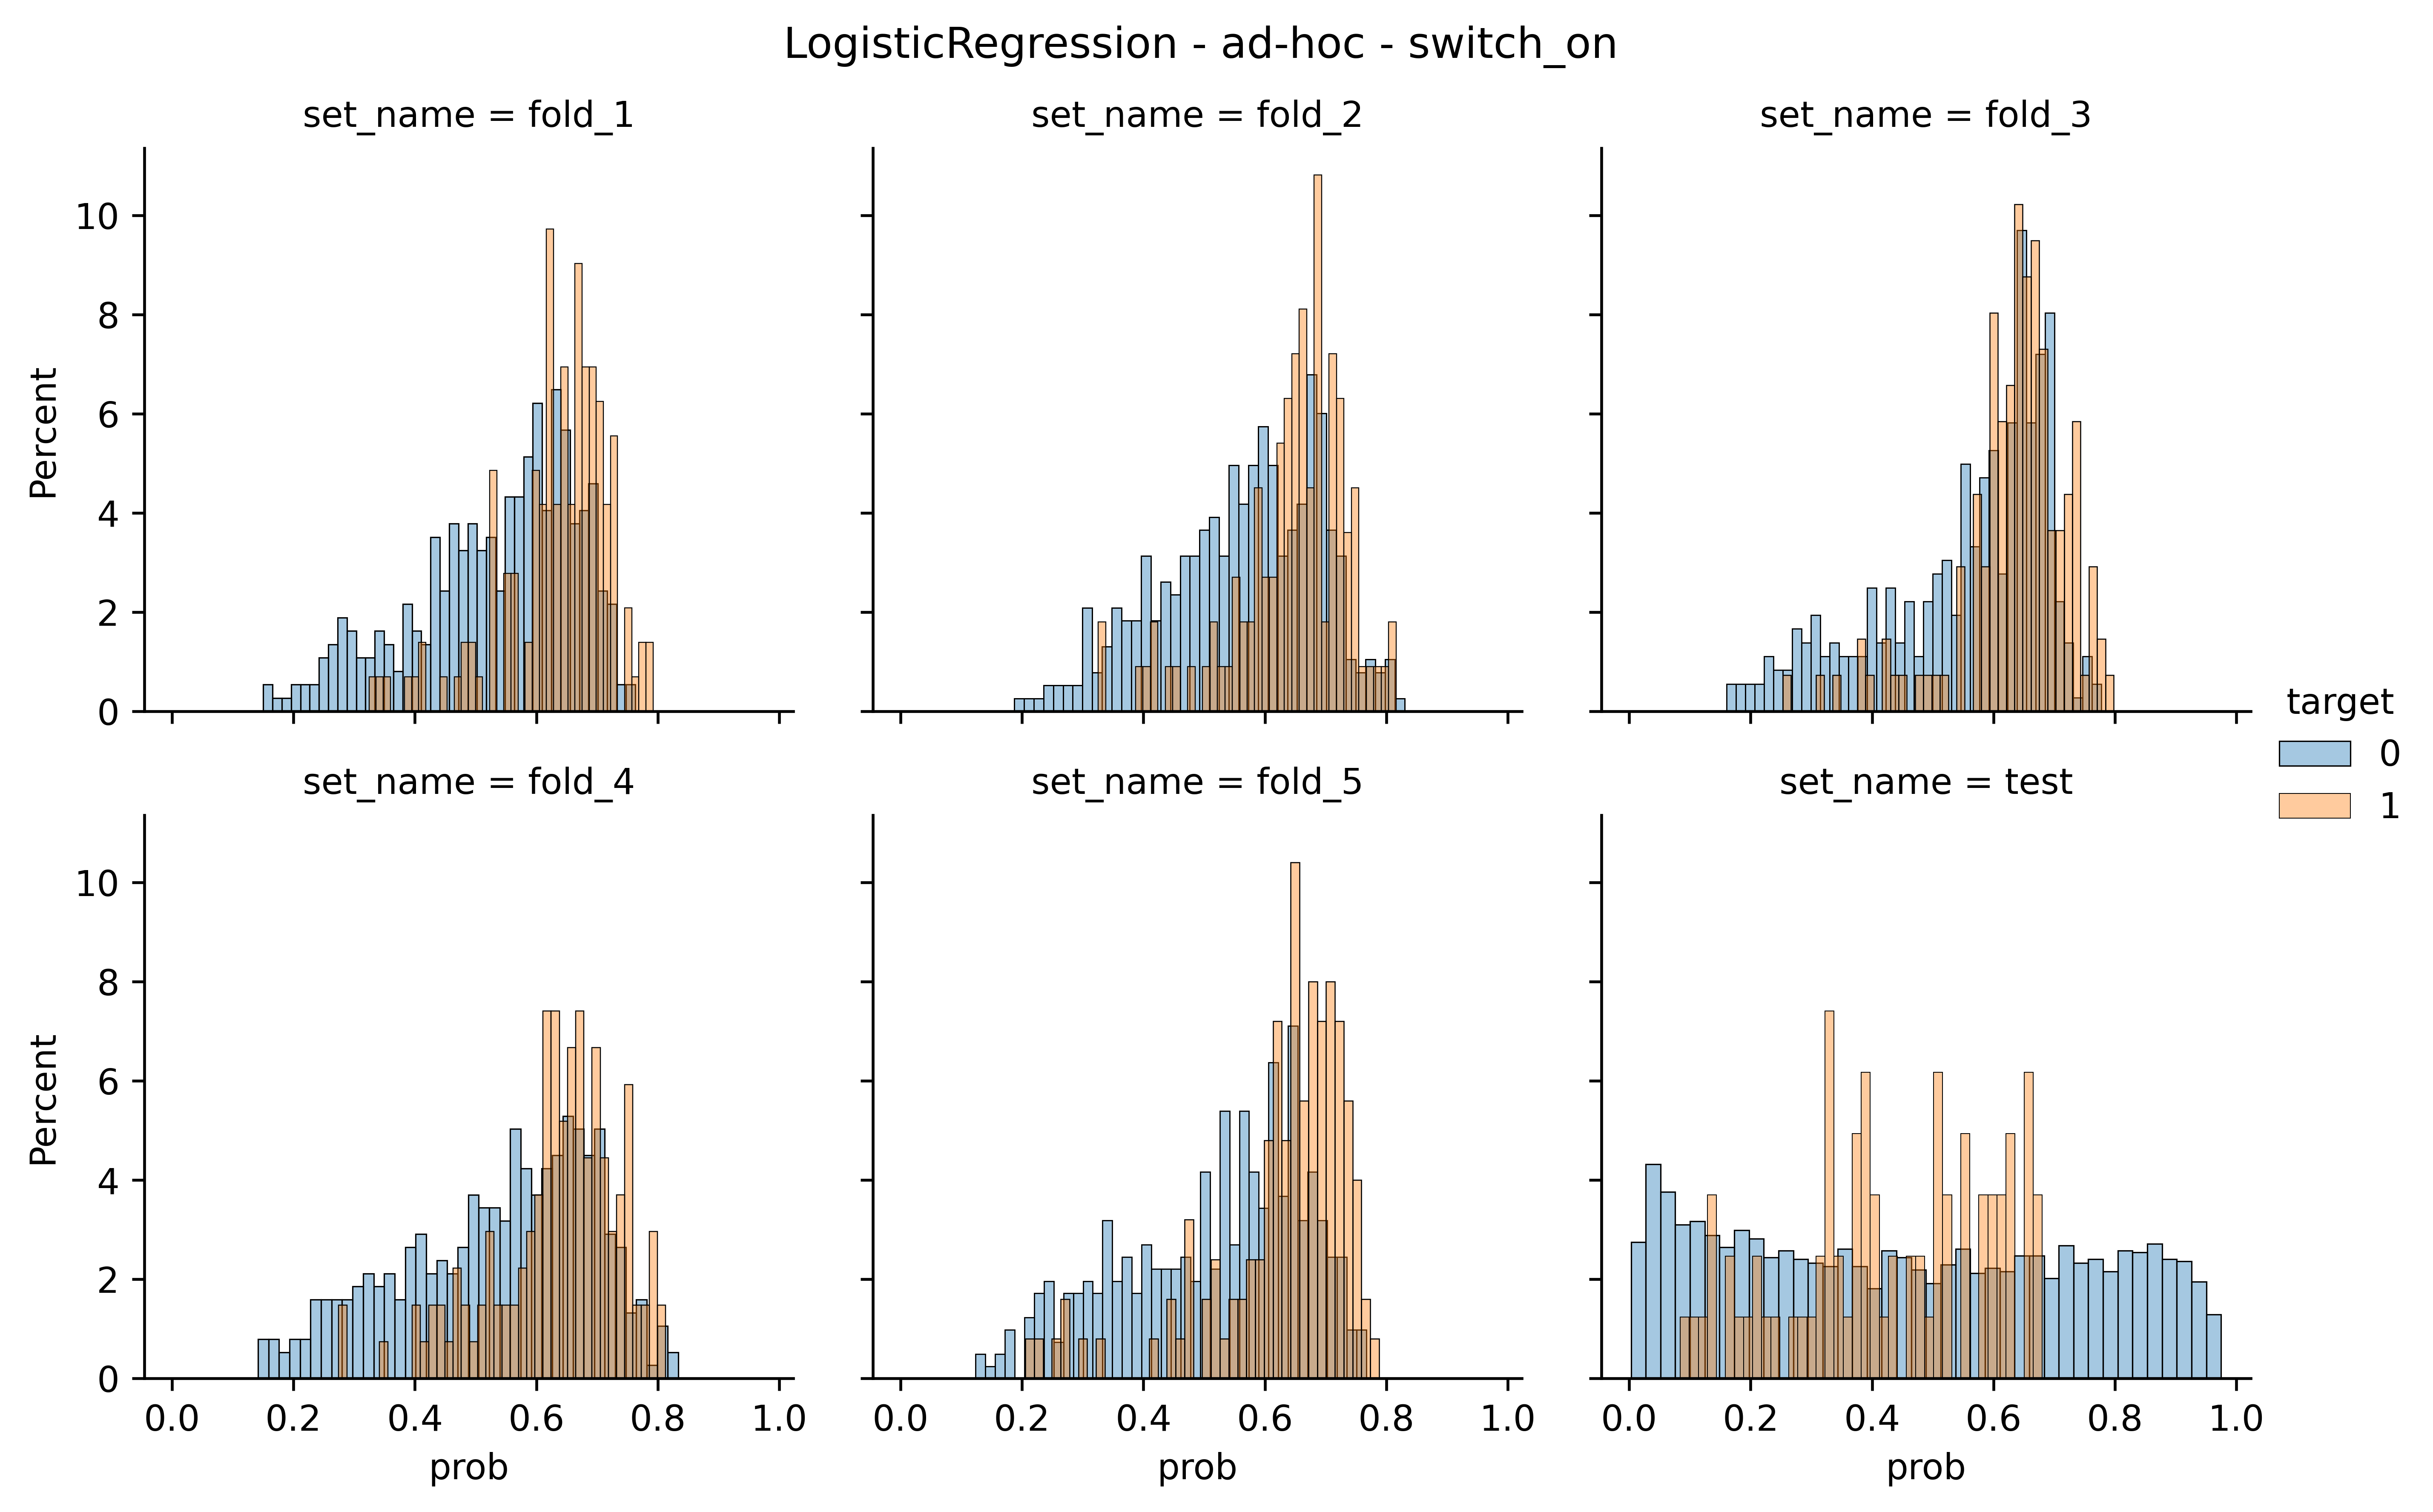
\includegraphics[width=\linewidth]{figures/results/ad-hoc/lgr/switch_on/turn_to__distplot.png}
%     \end{subfigure}
%     \hfill
%     \centering
%     \begin{subfigure}[b]{0.83\textwidth}
%         \centering
%         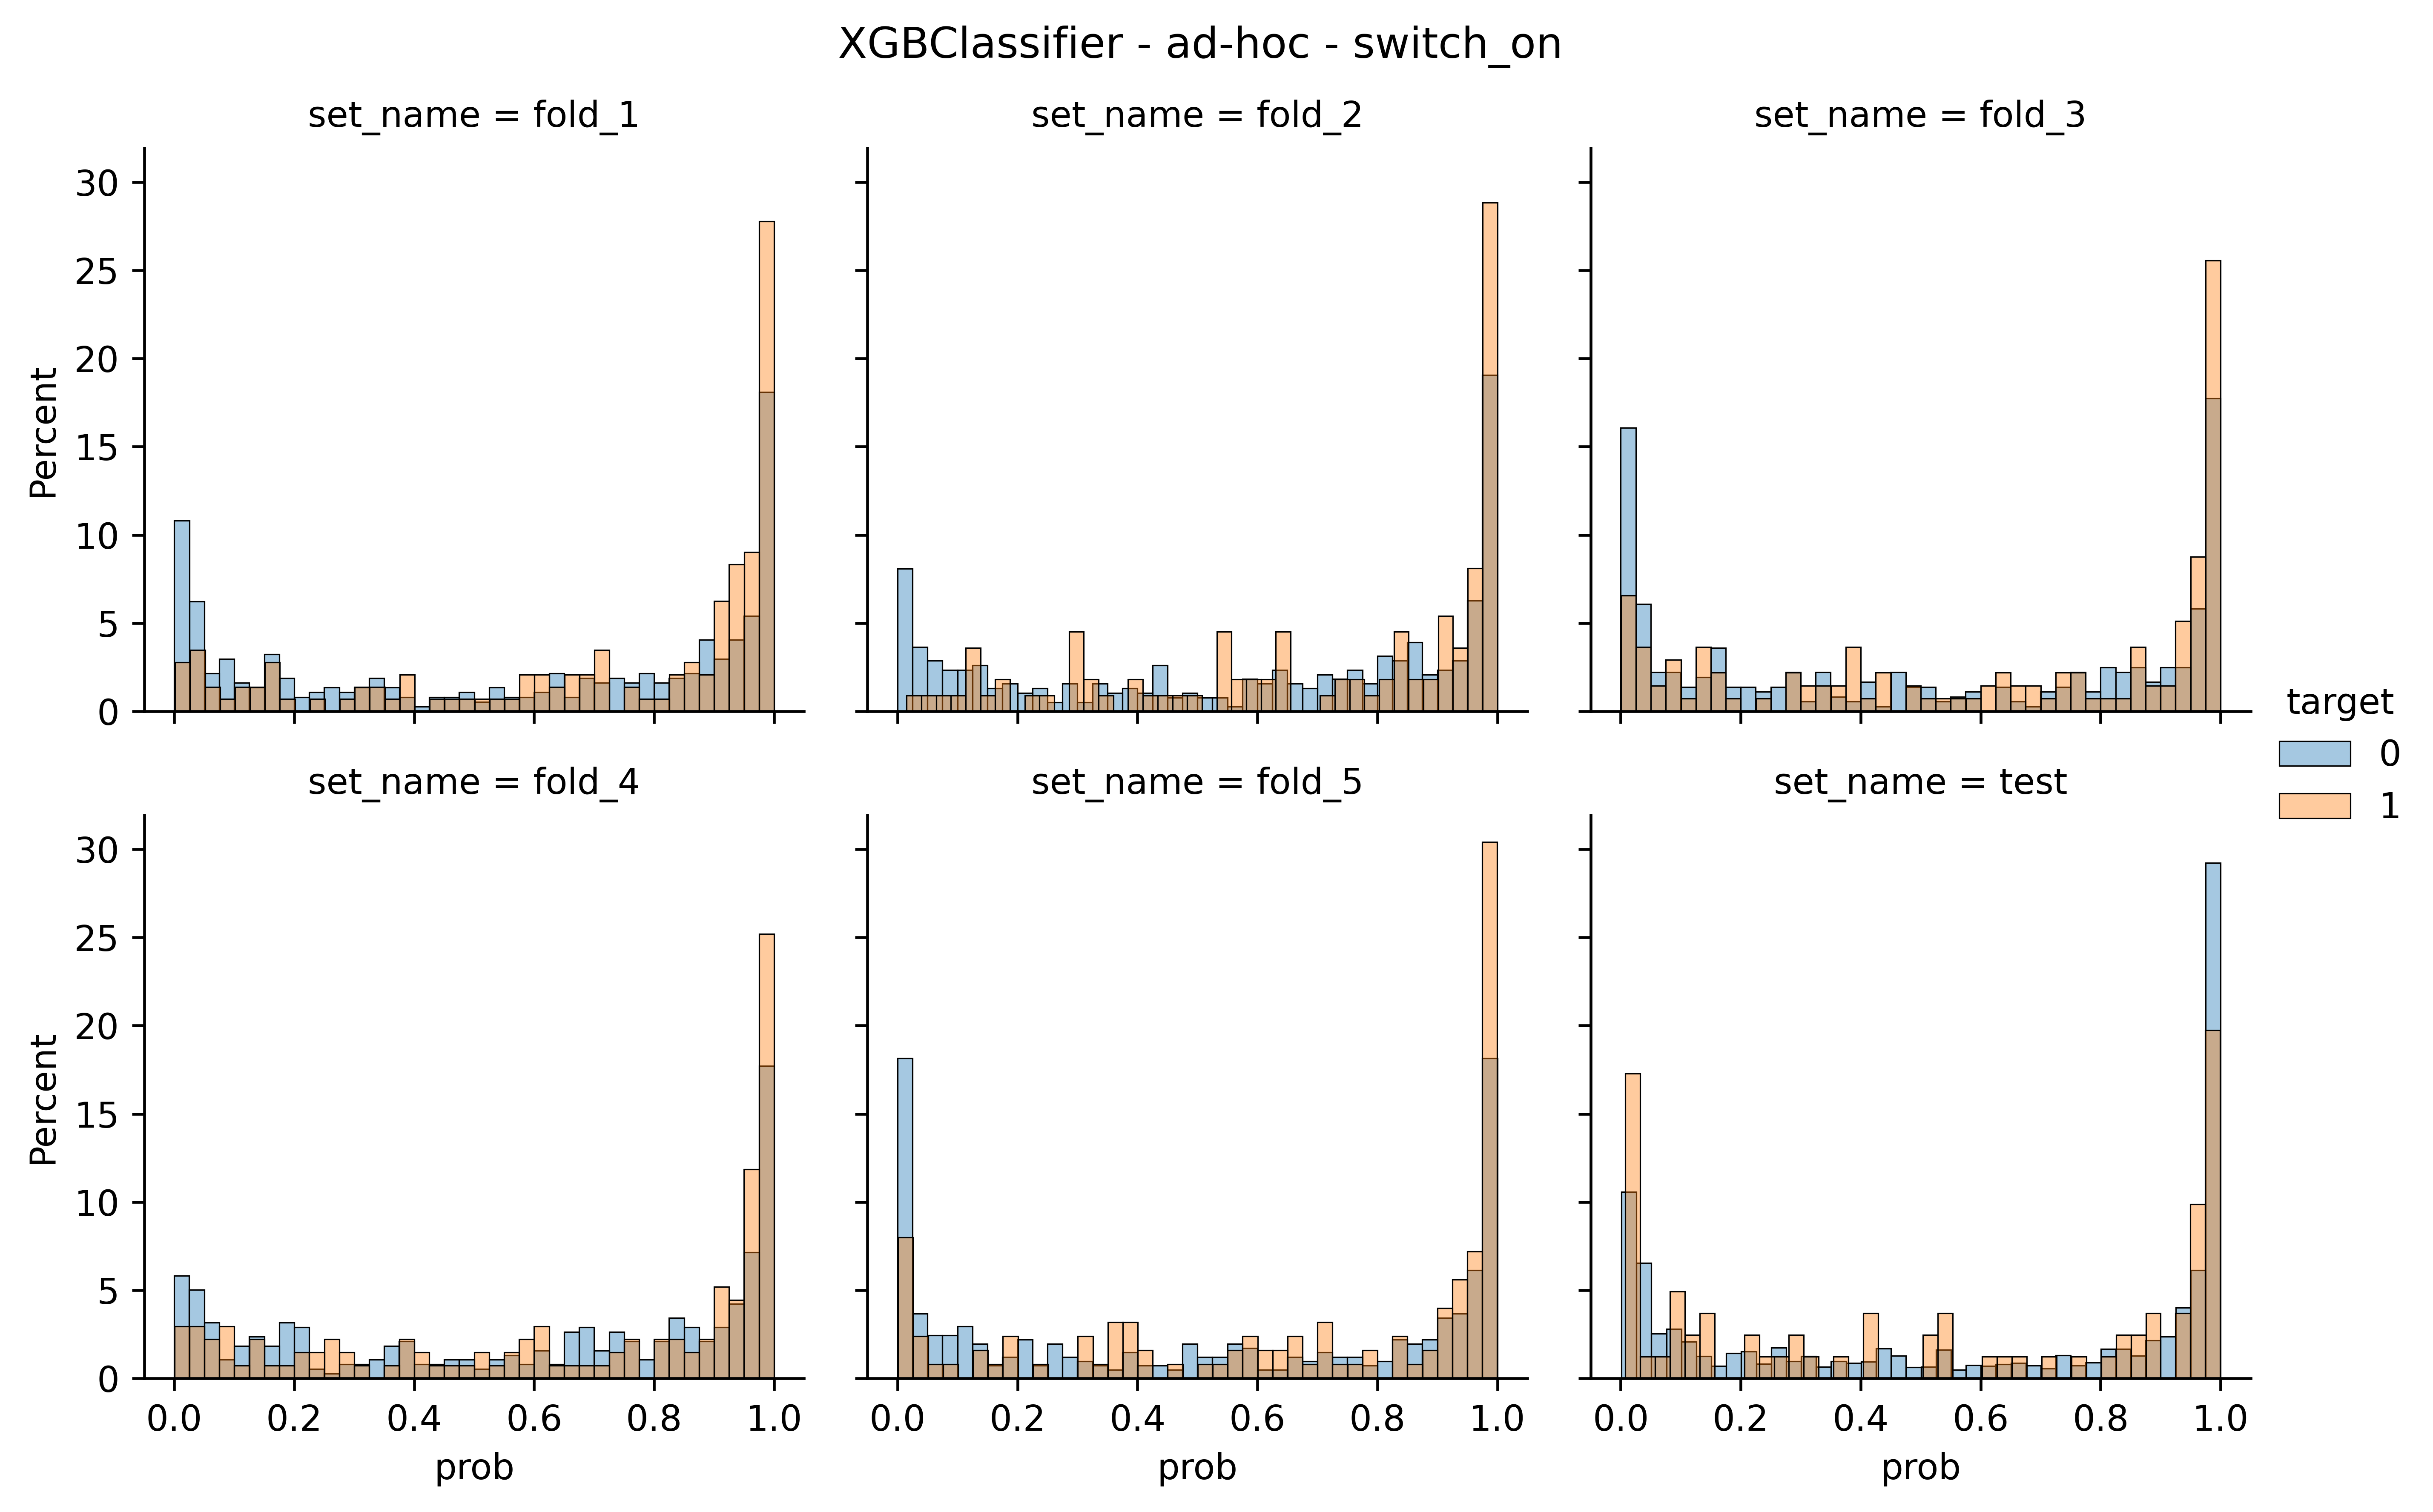
\includegraphics[width=\linewidth]{figures/results/ad-hoc/xgb/switch_on/2021-12-07_06.56.08.418411__distplot.png}
%     \end{subfigure}
%     \hfill
%     \centering
%     \begin{subfigure}[b]{0.83\textwidth}
%         \centering
%         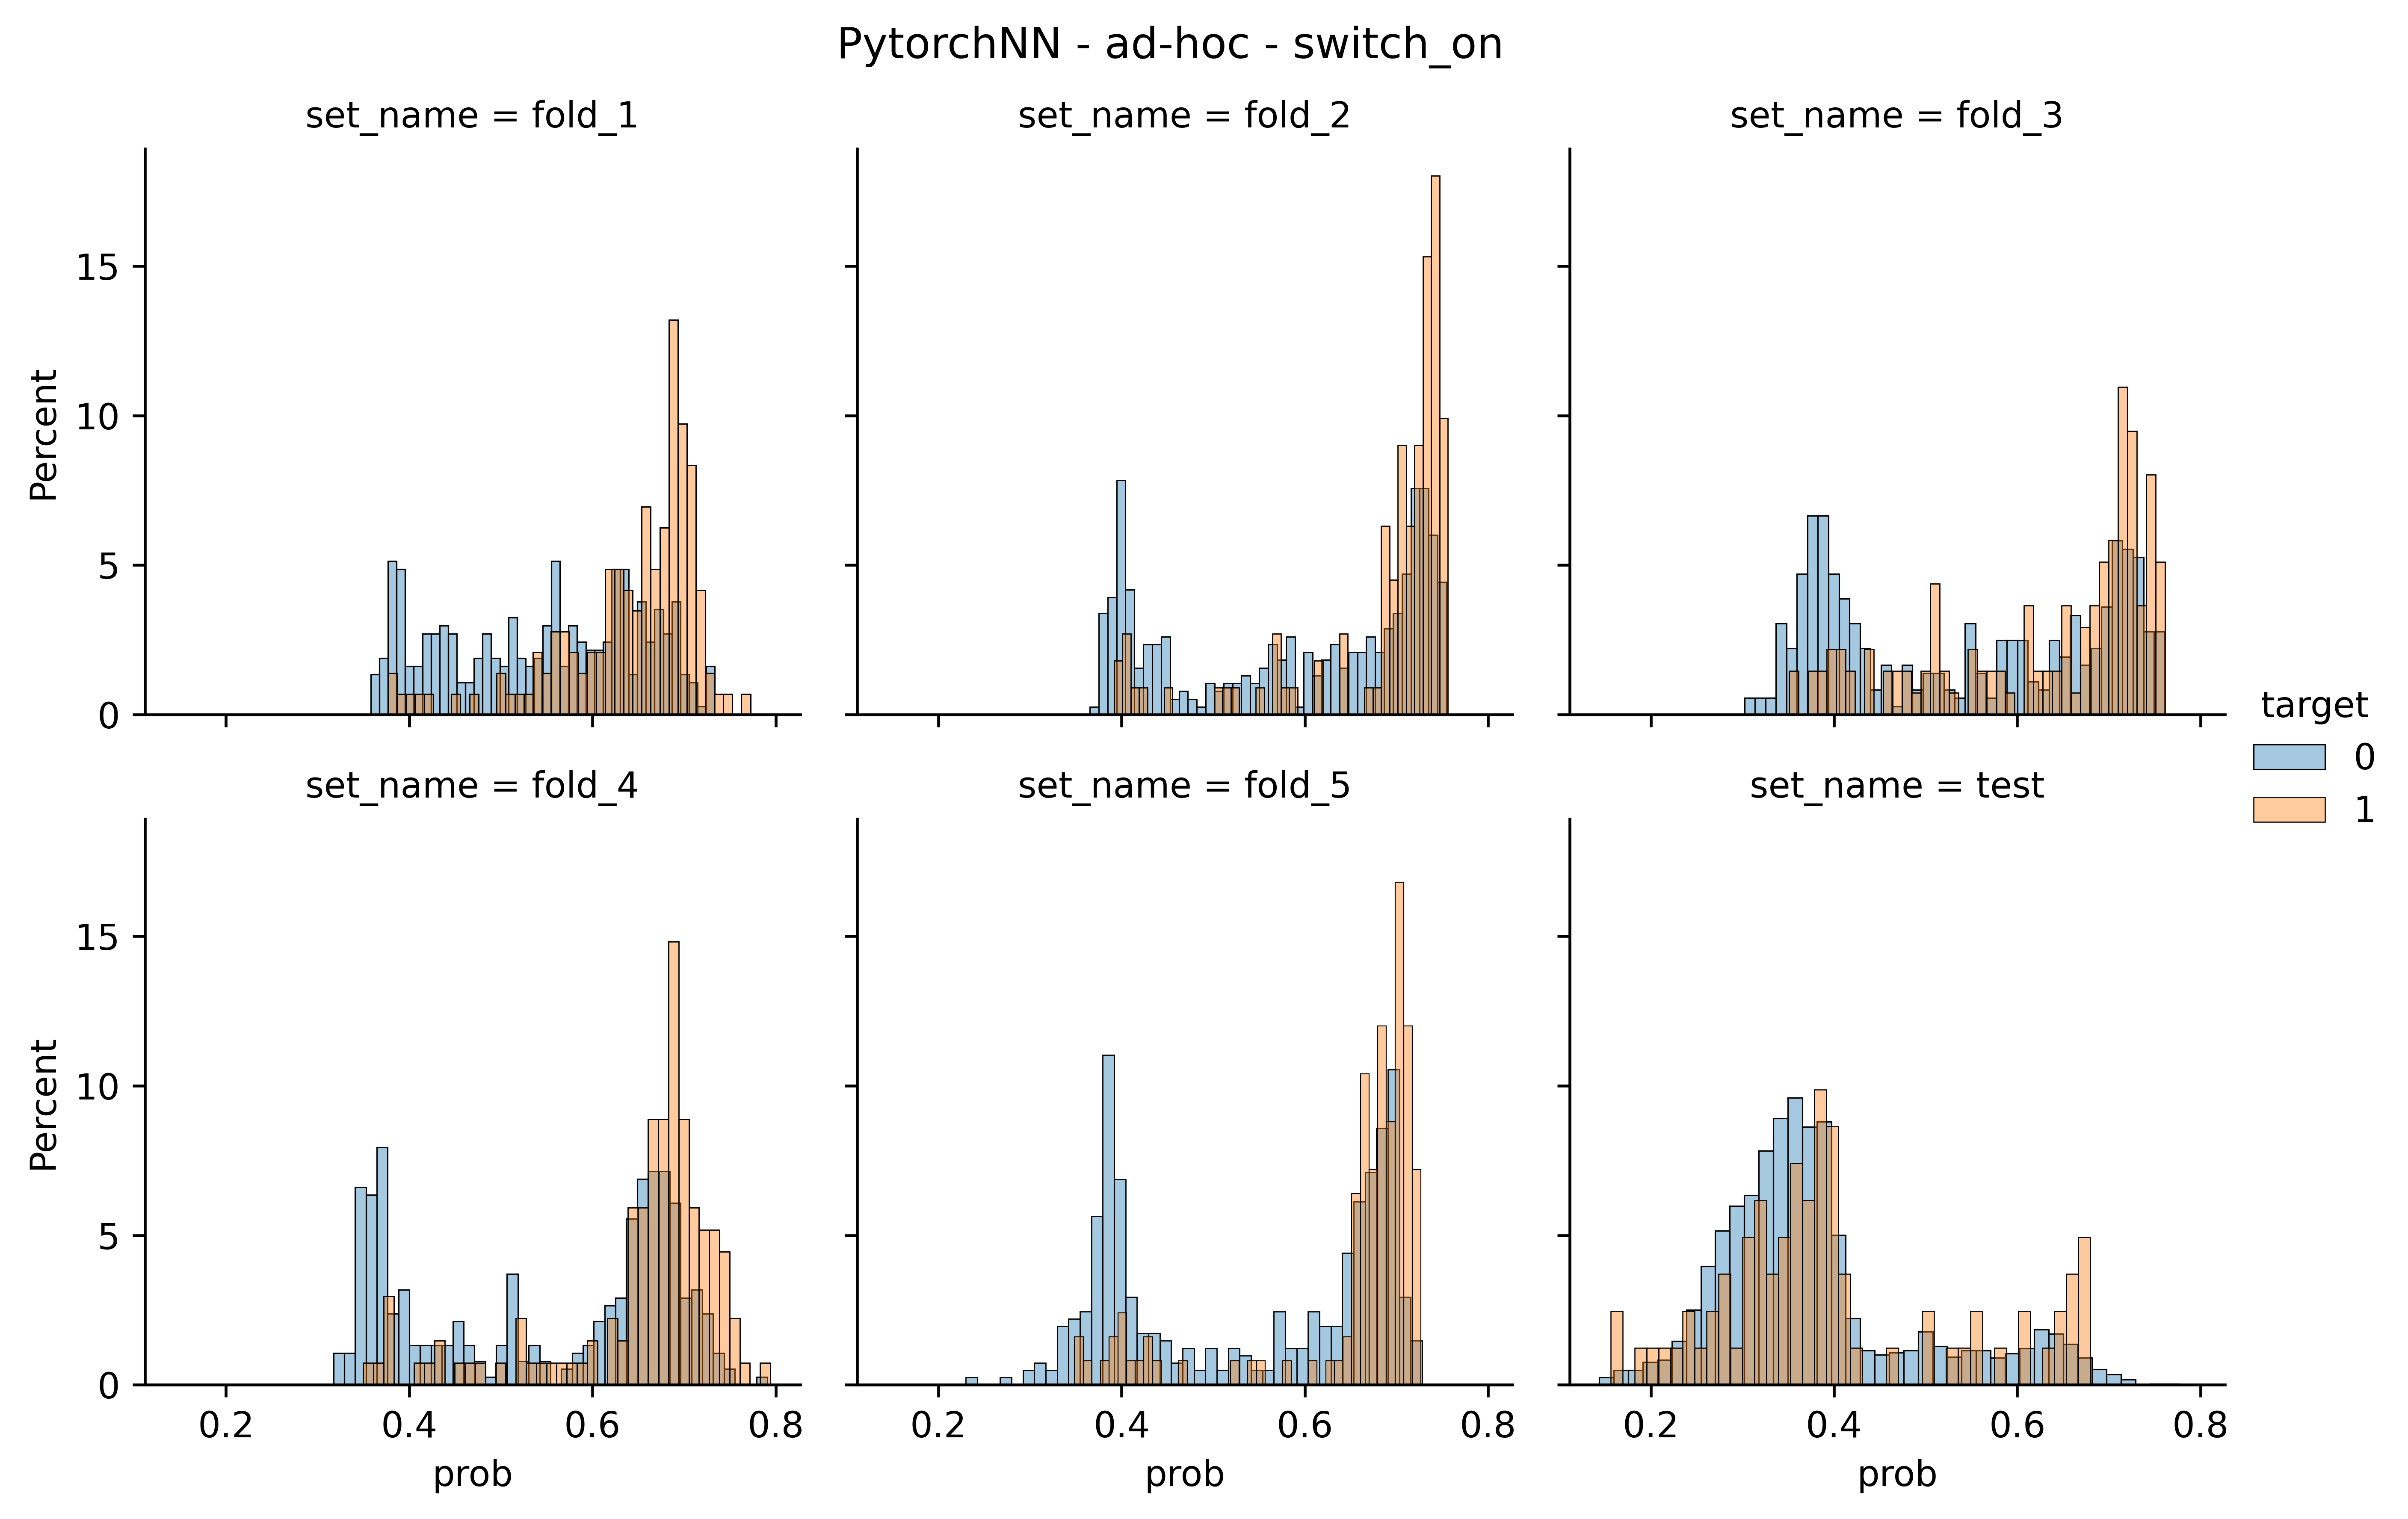
\includegraphics[width=\linewidth]{figures/results/ad-hoc/nn/switch_on/2021-12-06_18.44.35.478500__distplot.png}
%     \end{subfigure}
%     \caption{Ad-hoc switch\_on}
% \end{figure}
% 
% \begin{figure}
%     \centering
%     \begin{subfigure}[b]{0.83\textwidth}
%     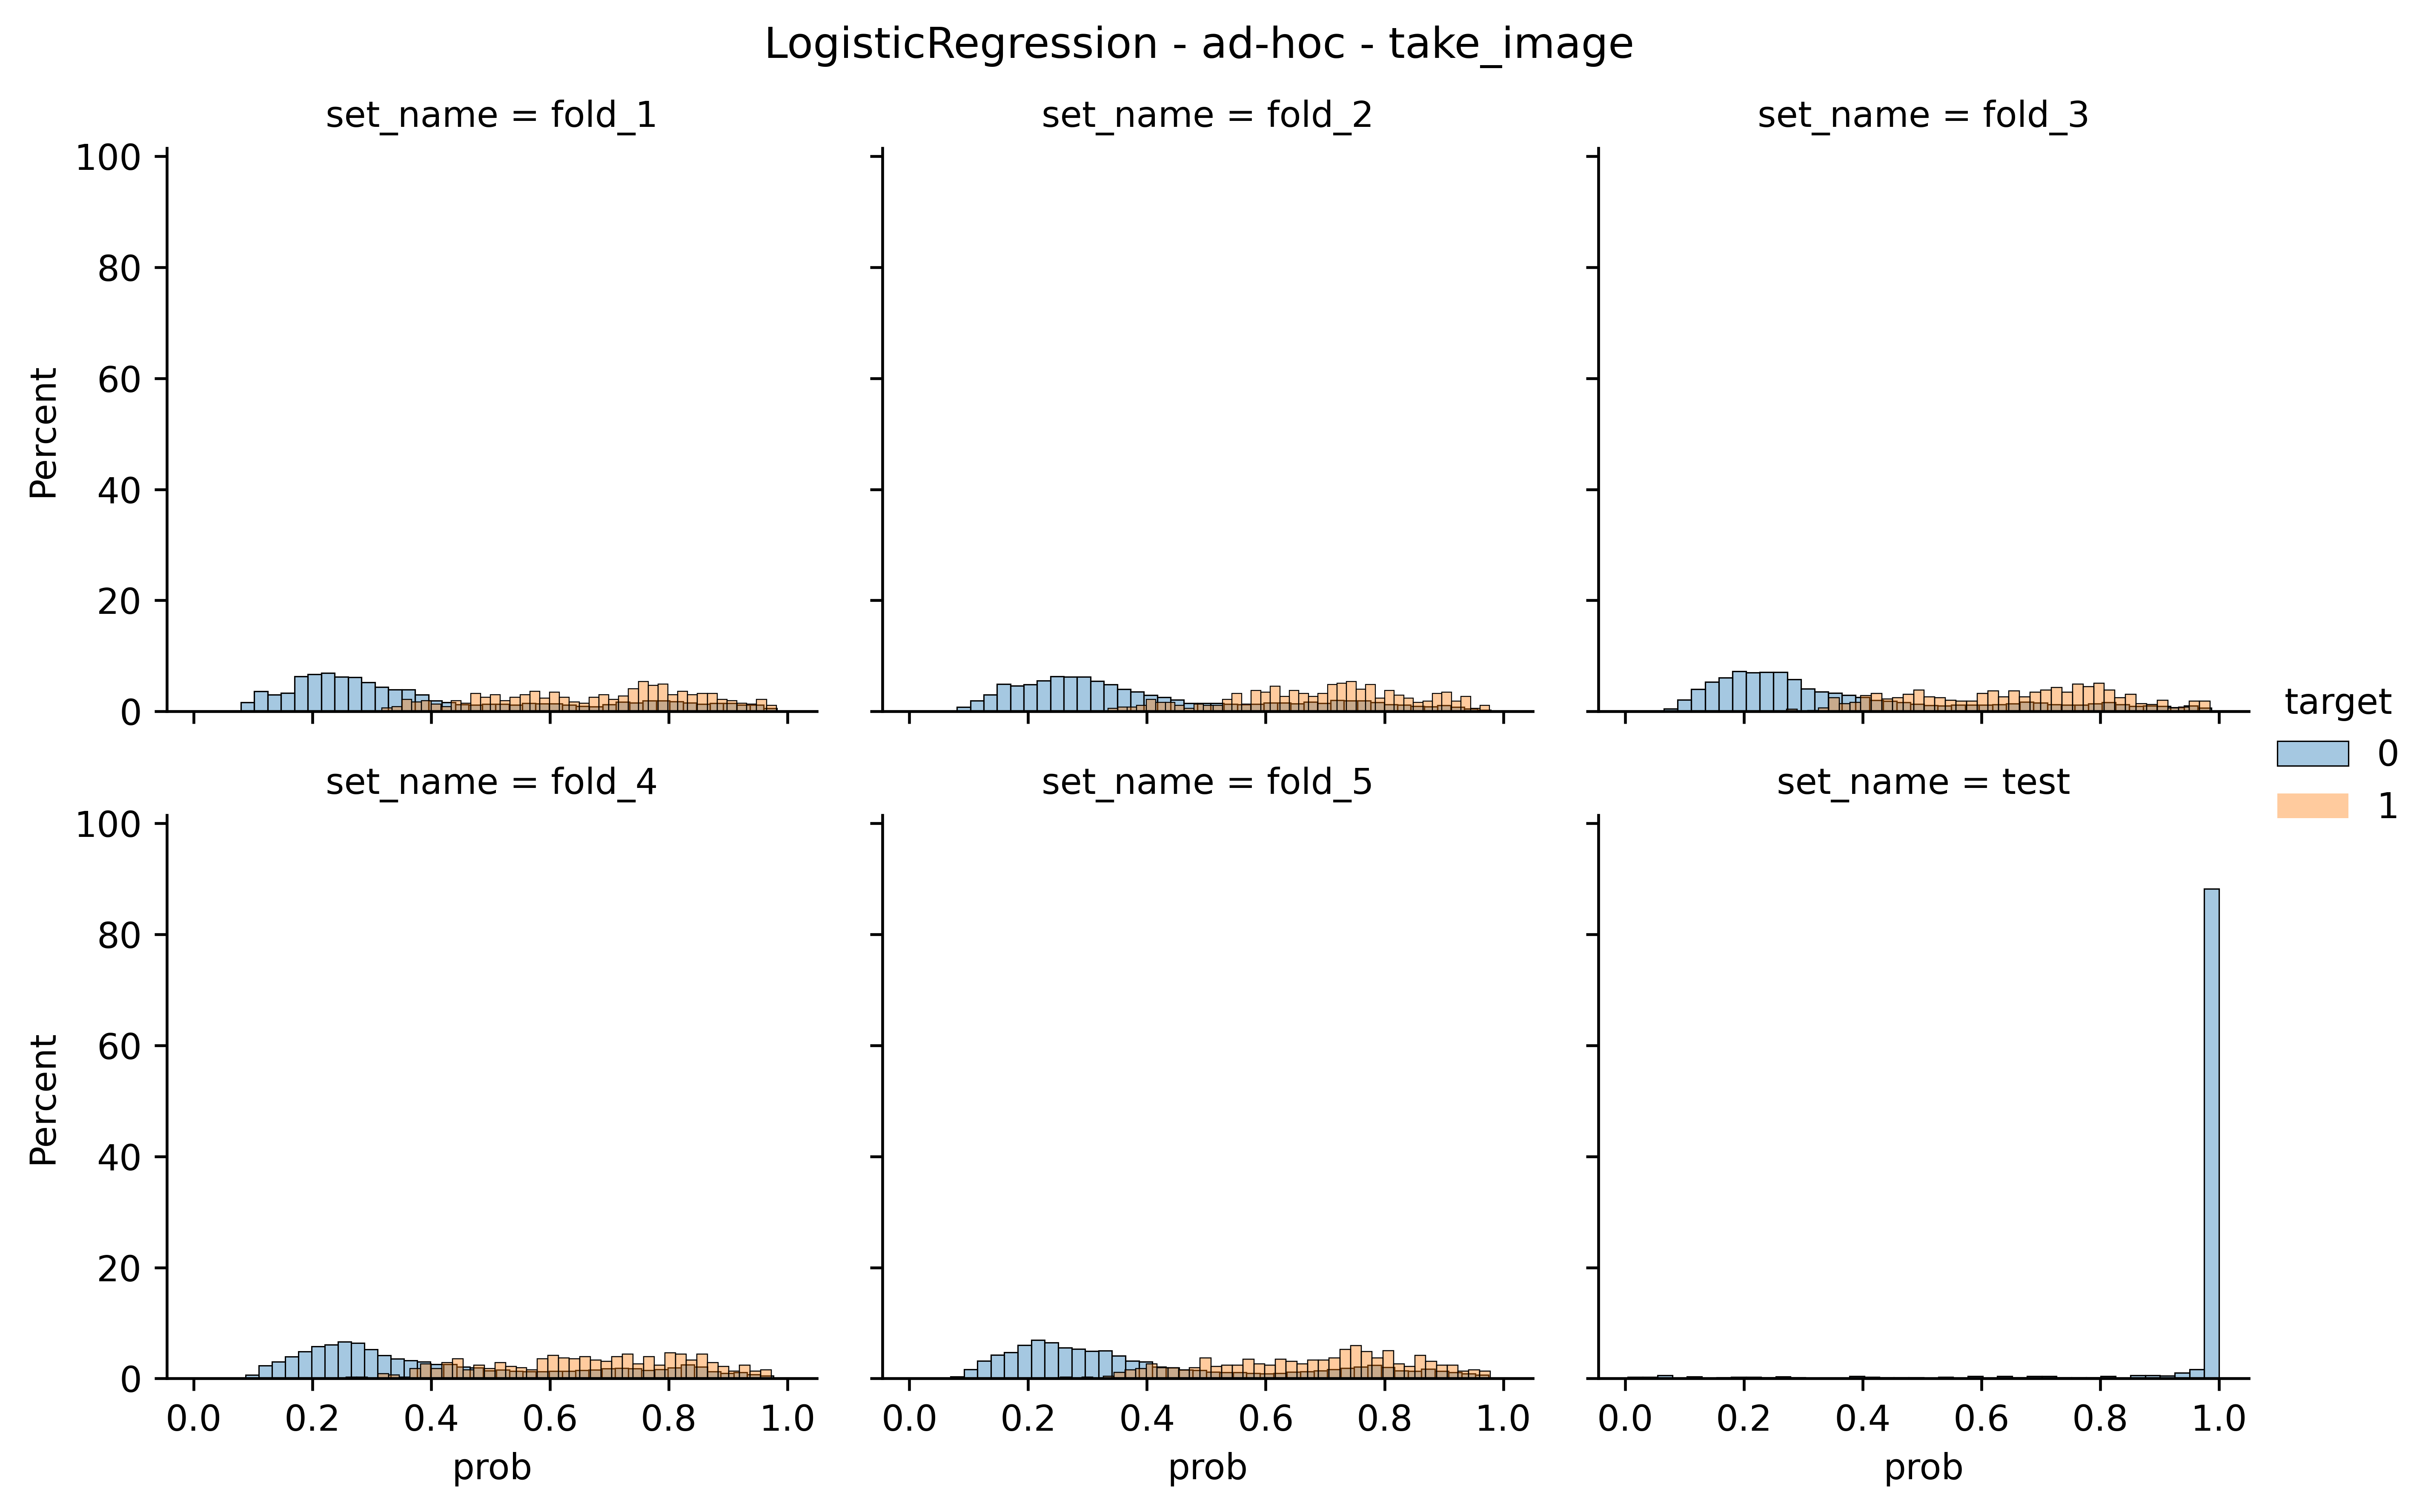
\includegraphics[width=\linewidth]{figures/results/ad-hoc/lgr/take_image/take_image__distplot.png}
%     \end{subfigure}
%     \hfill
%     \centering
%     \begin{subfigure}[b]{0.83\textwidth}
%         \centering
%         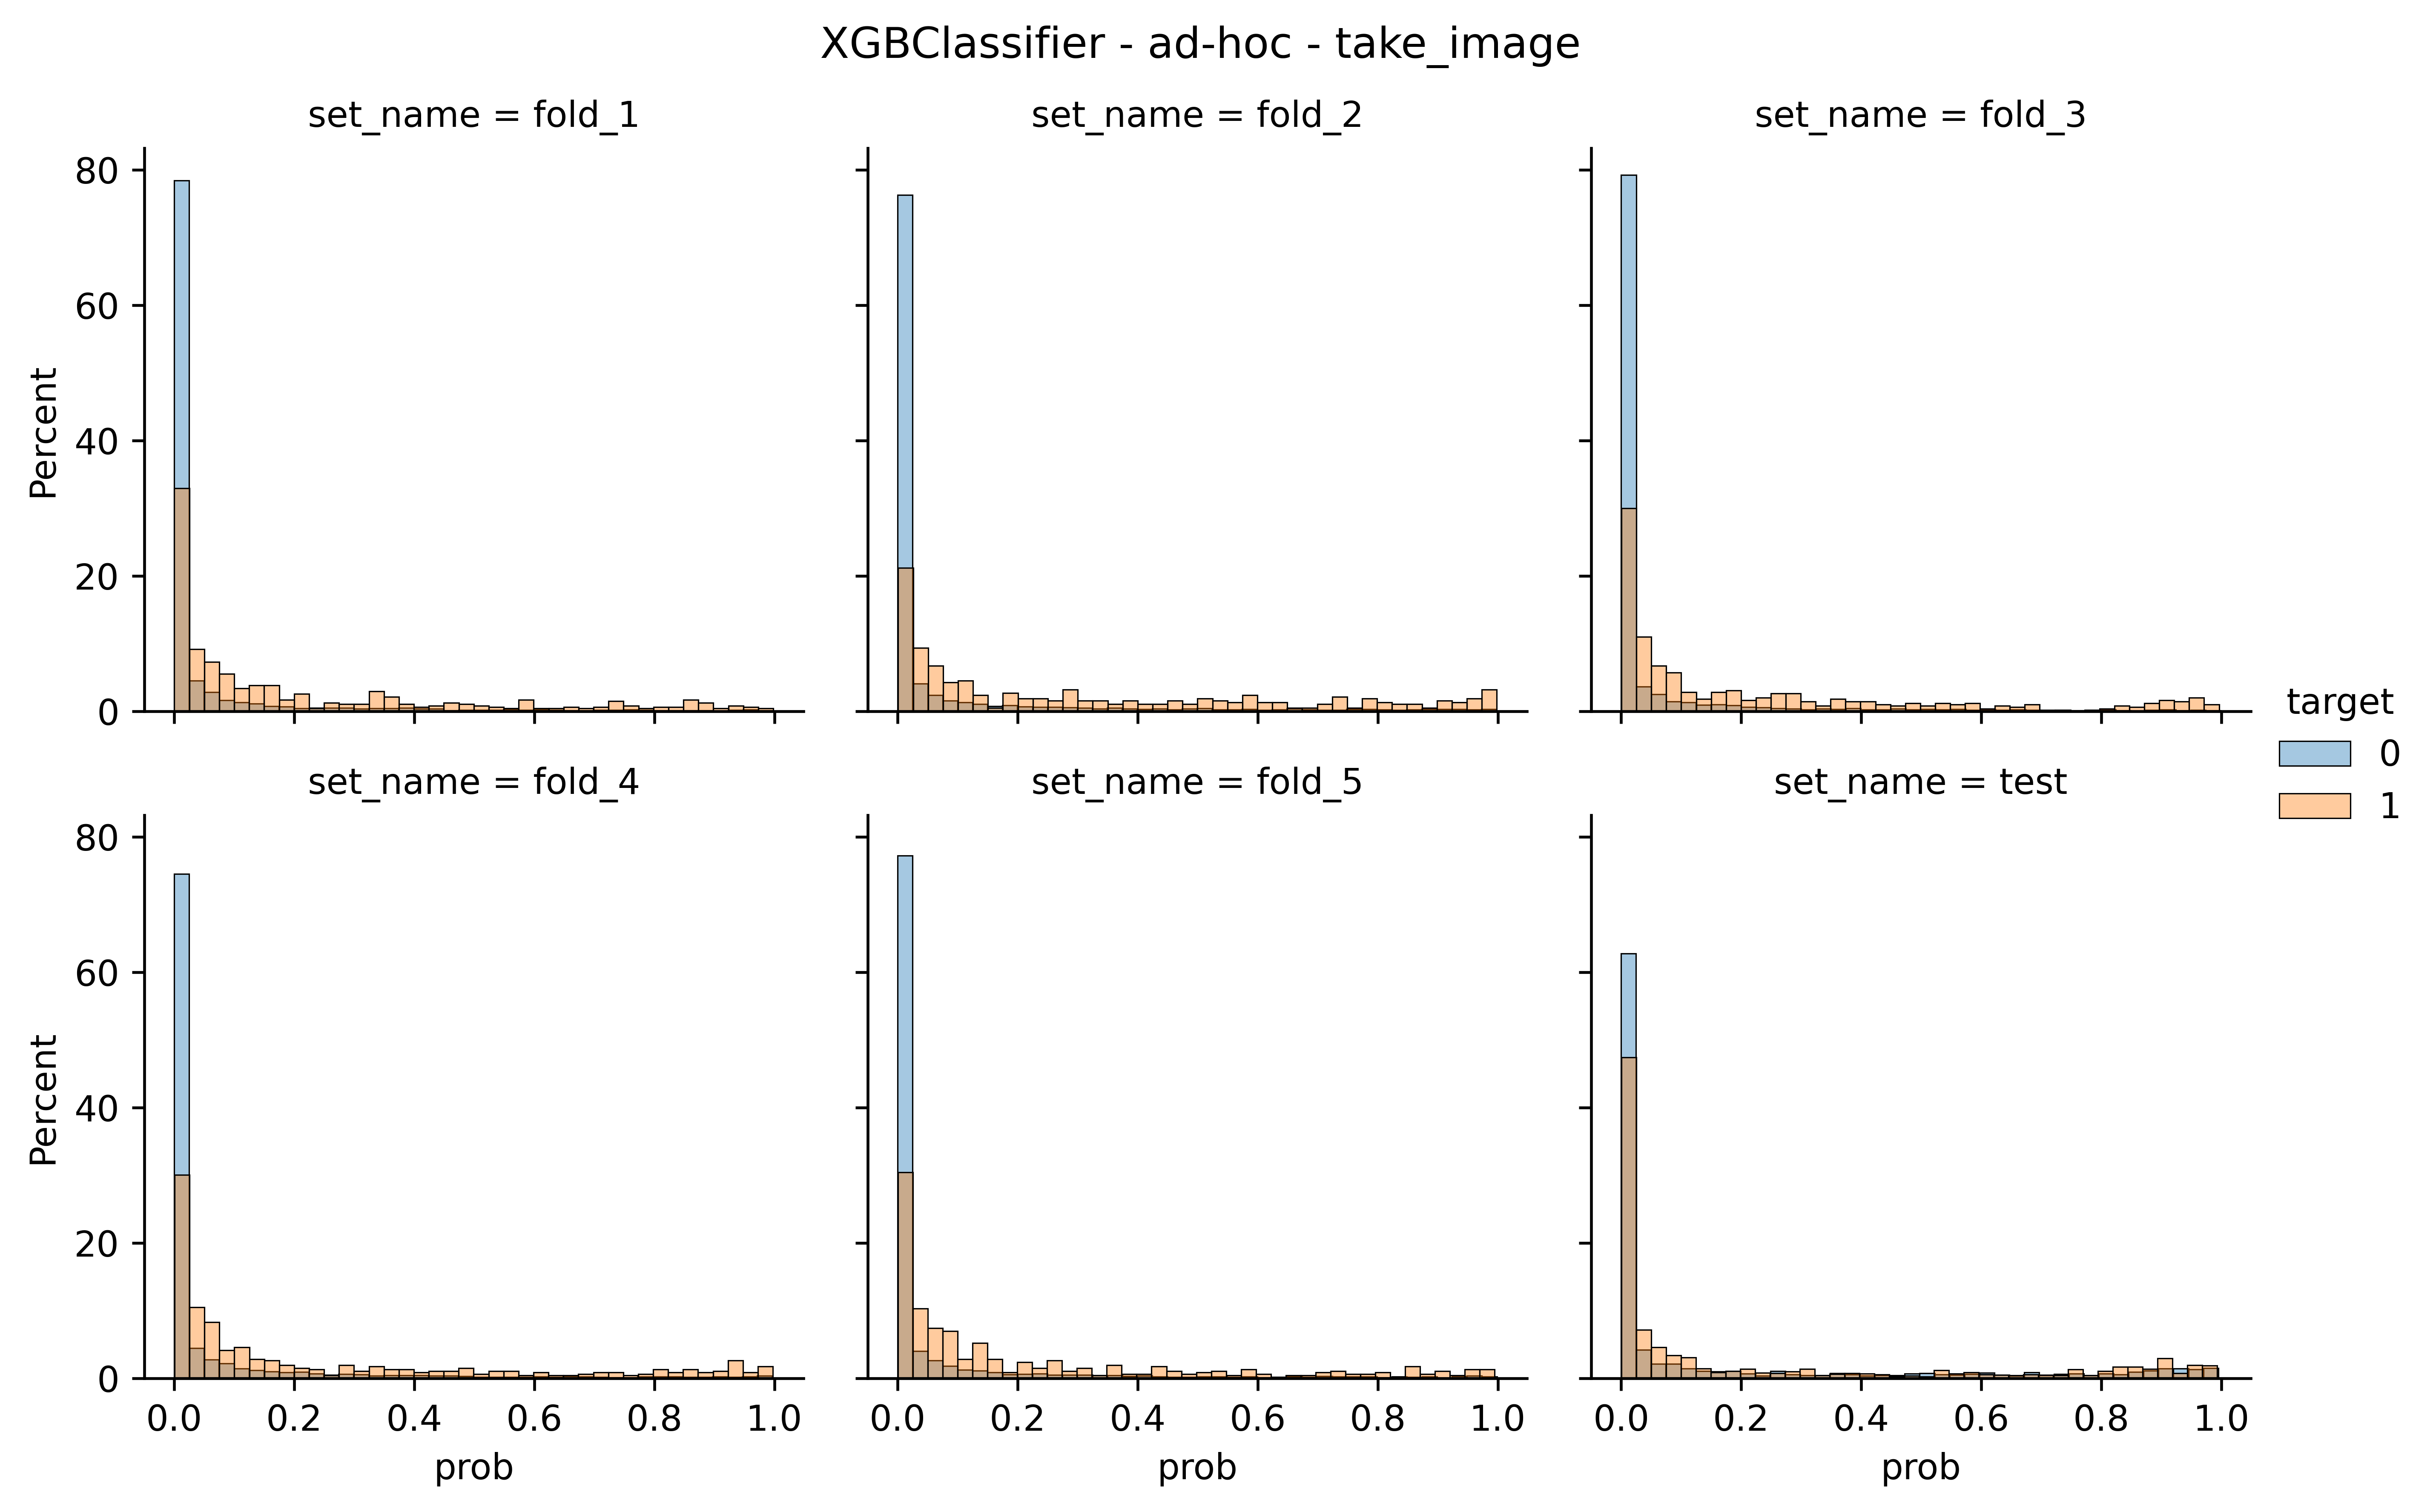
\includegraphics[width=\linewidth]{figures/results/ad-hoc/xgb/2021-12-07_07.38.35.967776__distplot.png}
%     \end{subfigure}
%     \caption{Ad-hoc take\_image}
% \end{figure}

% \section{Tiempos de predicción}
% \label{exp:time}
% 
% Para un nuevo ejemplo no visto se debe realizar el proceso completo creación de
% ventanas, codificación, predicción por parte del clasificador, y posterior
% agrupamiento de ventanas para obtener la máxima prioridad. Al incluir los
% modelos predictivos en el proceso de grounding heurístico el tiempo necesario
% para realizar todas las etapas y obtener el valor de salida del modelo
% predictivo es importante durante el proceso de grounding heurístico ya que los
% planificadores deben encontrar la solución a la tarea asignada de acuerdo a un
% tiempo límite, si este es excedido, ocurre una falla por parte del planificador.
% Esto motivo la medición del tiempo de respuesta para los modelos predictivos
% comparados en la sección \ref{results:comparison}.
% 
% Actualmente la implementación de grounding heurístico en Fast Downward, son
% realizadas a nivel de ejemplo. Por lo que la unidad de medida utilizada fueron
% \emph{ns/ejemplo}, no obstante también se probaron realizar las predicciones a
% nivel de batch con el de determinar que tan prometedor es incluir este cambio en
% el algoritmo de grounding heurístico.
% 
% \subsection{Predicciones por batch}
% 
% \subsection{Predicciones por acción}

\section{Otros experimentos}

Los experimentos presentados en las secciones \ref{exp:ad-hoc}, \ref{exp:wb}, y
\ref{exp:time} fueron aquellos principales y los que nos enfocamos durante la
tesis. No obstante, se intentaron otras vías de análisis que llevaron a 4
experimentos con el fin de lograr aquel modelo que nos permita guiar el proceso
de grounding. A pesar de no lograr resultados concretos fueron parte importante
del trabajo y otorgaron conocimiento invaluable para involucrarse más en el
dominio del problema.

\subsection{Modelos End-to-end}

End-to-end (E2E) models refieren a sistemas complejos representados por un único
modelo neuronal profundo ensamblando las capas de preprocesamiento y como capas
intermedias del modelo. En particular, este tipo de pruebas se realizaron en una
etapa temprana de la tesis donde la idea de generar ventanas de planes relajados
aún no se había investigado. En particular se experimentaron con modelos E2E de
FastText donde agrega una capa neuronal más al modelo de embeddings para que
sean utilizados en clasificación. No obstante se optó por descontinuar estos
experimentos al comenzar ya que fueron experimentos prototipos donde se buscaba
verificar la factibilidad del uso de word embeddings en grounding heurístico.

\subsection{El problema de inclusión sobre planes relajados}

Otra estrategía que utilizamos durante el análisis en la generación de ventanas
de planes relajados, fue plantear el problema de clasificación binaria como uno
multiclase. En lugar de solo 2 clases, manteníamos 4 que representaban la noción
de si una acción estaba incluido en el plan relajado y si eran parte de los good
operators del problema. Es decir, una ventana de plan relajado $w$ y acción $a$
es etiquetada como:

\begin{itemize}
    \item 0: Si $a$ no es good operator y no pertenece a $w$.
    \item 1: Si $a$ no es good operator y pertenece a $w$.
    \item 2: Si $a$ es good operator y no pertenece a $w$.
    \item 3: Si $a$ es good operator y pertenece a $w$.
\end{itemize}

Luego al agrupar por ventanas y acción, consideramos como predicción final la
clase $3$ si al menos una de las ventanas predijo $3$. Caso contrario si para
alguna ventana la predicción fue $2$ predicción del agrupamiento es $2$. Y así
sucesivamente hasta la clase $0$.

\subsection{Mayorización}

La repetición de ejemplos con etiquetas diferentes puede dificultar el
aprendizaje de un modelo, si no son preprocesadas con alguna técnica de
mayorización. Es decir, de entre todas las repeticiones del mismo ejemplo pero
con distintas clases, mantener una sola replica preservando la etiqueta que haya
ocurrido en mayor cantidad. Esta técnica fue aplicada para la codificación por
word embeddings, donde una hipótesis para mejorar la separación de los ejemplos
de entrenamiento fue asignar la etiqueta mayoritaria para todo los vector de
dimensión $D$ (plan relajado, acción) que estén cerca en un rango en
$\mathbb{R}^{D}$.

\subsection{Orden de ventanas como características}

Por último otra implementación que se agregó al sistema y que es un patrón
configurable de las etapas de ejecución es la posibilidad de mantener el orden
en que ocurren las ventanas. Es decir, se tiene

\begin{table}[h!]
\centering
\scalebox{0.9}{
 \begin{tabular}{||c | c | c | c||} 
 \hline
 Plan relajado & Orden de ventana & Acción & Etiqueta \\ [0.5ex] \hline\hline
 %(take_image satellite0 planet5 instrument1 image1)
 {}[] & 1 &{}[] & 1 \\
 {}[] & 2 &{}[] & 1 \\
 {}[] & 3 &{}[] & 1  \\
 ... & ... & ... & ...\\ [1ex] 
 \hline
 \end{tabular}}
 \caption{Ejemplos etiquetados a partir de un plan relajado y una acción}
 \label{tb:matrix_shape}
\end{table}

El objetivo de este agregado es evitar perder la información del orden durante
la separación y se buscaba analizar si es un factor relevante para el
entrenamiento y evaluación.